\chapter{Framework testing and `partial' model results \label{chapter:models}} 

\section{Introduction}

\subsection{Organisation of the chapter}

This chapter presents results from the model framework. It does this in five sections with the following aims:

\begin{itemize}
	\item Test that the main economic components of the model function correctly, first without any spatial element, and then with space costs included;
	\item Test the difference between using a `hill-climber' vs ‘constrained' utility approach;
	\item Provide People with mobility and a density cost to investigate partial economic outcomes when People optimise;
	\item Give Firms mobility to investigate their ability to maximise revenue and to examine the \gls{dmr} issue.
\end{itemize}

%These aim to give an initial intuitive sense of what the model is showing, before going on to present the relevant data output. The visualisation can be as good a data summary as graphed data output, since it can be easier to see what is fundamentally happening through these than in the data, in much the same way that any map can enable a good overview.
%It will be made clear in the text where a model output or analytic approach is being discussed.

\subsection{Presentation of results \label{sec:resultspresent}}

In this and the following chapter, results and analysis are presented graphically in four ways:

\begin{itemize}
	\item Model run results include:
\begin{itemize}
	\item $(1)$ A visualisation from the model thesis framework. These are screenshots from the `live' code; versions of the same results can be downloaded via the link provided in the code appendix (\ref{apx:modelcodeoverview}), where parameters can be varied;
	\item	$(2)$ Graphed data output from a model run
\end{itemize}
	\item $(3)$ Analytic results, where particular features are analysed mathematically to understand how a key model feature functions;
	\item $(4)$ Spreadsheet versions of model dynamics are used in two cases. These boil down model dynamics to their most essential, simplified components in order to understand what is driving the emergent behaviour seen in the model framework. One appears in section \ref{sec:rationalchoices}, explaining how the optimal choices of People drives spatial outcomes in the `mobile People' models. The other is used in the transmission belt chapter (section \ref{sec:lov_vs_eos}) to understand how People's demand can determine the transition between production regimes.
\end{itemize}

Each visualisation is designed to make a specific point about the model it shows; a full description of them is given in the sections in which they are used. Figure captions repeat this information in a compacted form to give an accessible summary where they appear. 

Correlations from the model framework are used extensively throughout the results. While the basic principle applies to all of these (showing how two quantities are dependent), the data points themselves vary depending on the purpose of the correlation being shown. Again, these are explained in detail in the captions for each, but it is worth mentioning the different ways these correlation graphs will be used:

\begin{itemize}
	\item Datapoints will show separate agents, correlating two variables for each of them at a given point in model time.
	\item Single variables (e.g. the distance cost for all agents) will be correlated against other single variables. Often, one of thes will be the mean taken from all agents for a given variable.
	\item Datapoints will be taken at specific `trigger' points in model time, for example in the `mobile People' models, when Person movement drops below a set value and `spatial equilibrium' is assumed to have been reached.
	\item In one example only (section \ref{sec:tbmplusdensity}), datapoints are taken on each model timestep for a timespan of interest. Here, the direction of model time is indicated in the correlation by using arrows for datapoints.
\end{itemize}

A more mathematical analysis is used in two types of situation. Firstly, many of the basic dynamics of the model are best communicated using an analytic approach. Secondly, when the model framework produces results that require further explanation. When the agent model outputs a particular outcome, is it due to Actors acting rationally? If so, what factors are at work? The framework proposes these questions, but a full answer may require an analytic comparison. Where results of such an comparison are informative, they have been  included. As discussed in the conclusion, this is a happy synergy: the  agent model helping to highlight possible lines of inquiry, and an analytic approach  shedding further light on the issues. It will be made clear in the text where a model output or analytic approach is being discussed.

The use of stochastics varies depending on the presentation. Some results rely on stochastics to illustrate a point; others present only one model run outcome without showing all stochastic outcomes. For example, a number of the transmission belt presentations show a specific outcome, with emergent producers in a particular region. The specific outcomes are random, but for the purposes of clear presentation, one is shown. Other model presentations (e.g. in section \ref{sec:mobFirms}) present stochastic outcomes; these are explained where they are presented.

%These aim to give an initial intuitive sense of what the model is showing, before going on to present the relevant data output. The visualisation can be as good a data summary as graphed data output, since it can be easier to see what is fundamentally happening through these than in the data, in much the same way that any map can enable a good overview.

\section{Testing utility functions \label{sec:testingutils}}

This section demonstrates that the model framework successfully replicates the basic micro-economic ideas outlined in chapter \ref{chapter:location}. This is done by initially excluding any spatial elements to keep a clear focus on the central economic functions themselves. The aim is to demonstrate the robustness of the underlying utility concepts before introducing further model complexities.

\subsection{CES function}

The discrete-good \gls{ces} function \eqref{eq:-6} is most commonly used in the models that follow. Section \ref{sec:utilspace} explores the interaction of the \gls{ces} function with space; the function's basic output is tested here. 

The following uses a model run test (see figure \ref{fig:CEStestResults}) that removes all spatial costs and normalises wage to 1 and all good costs also to 1. A single Person then optimises: what optimal mix of goods can they buy? Firstly, this is done for $0<\rho<1$, in a situation with two goods. (Recall that as $\rho \rightarrow 1$, goods become substitutes and \gls{lov} drops.) Two views of that data are given, since for $\rho<0.2$, utility becomes very large. Sub-figure \ref{fig:ces13} illustrates that, as $\rho \rightarrow 1$, utility from a wage of 1 for two goods moves towards 1. When $\rho=1$ all goods are subtitutable, so any mix would produce the same utility value.

Secondly, in sub-figure \ref{fig:ces11}, $\rho$ is held at $0.75$ and the number of goods (in the model, the number of supplying Firms) is changed, up to a thousand. Each good has the same price, so the optimising Person buys a symmetric mix of all available varieties. While the budget constraint does stop utility from growing exponentially with varieties, it can be seen that utility increases (at a decreasing rate) as the number of goods consumed increases.

\begin{figure}[p]
\centering
\subfloat[2 goods, $\rho$ varied]{\label{fig:ces12}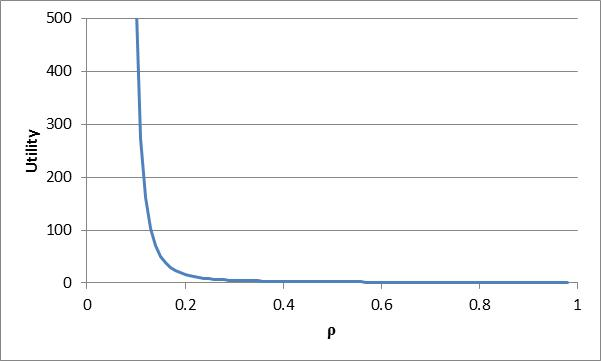
\includegraphics[width=0.7\textwidth]{ChapterTestingModels/Figures/CES2firm_rhochange1}}
\hspace{0.1}  
\subfloat[2 goods, $\rho$ varied, from $\rho=0.2$]{\label{fig:ces13}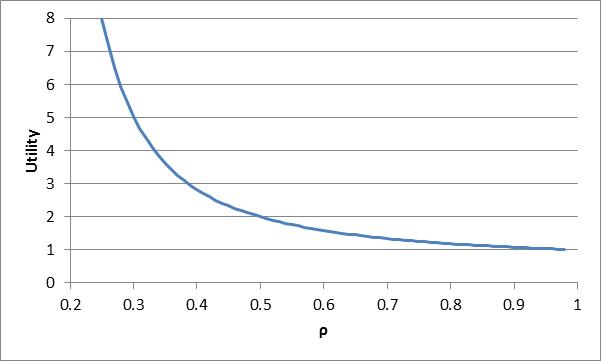
\includegraphics[width=0.7\textwidth]{ChapterTestingModels/Figures/CES2firm_rhochange2}}
\hspace{0.1}  
\subfloat[$\rho=0.75$, good number varied]{\label{fig:ces11}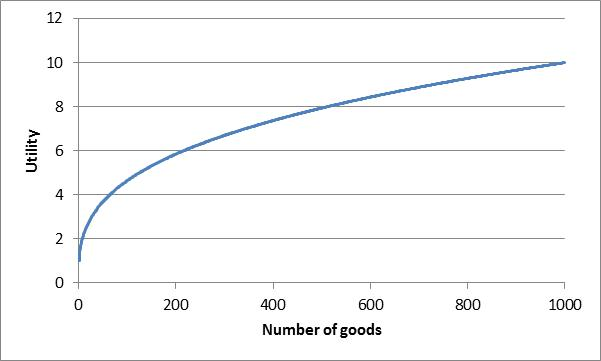
\includegraphics[width=0.7\textwidth]{ChapterTestingModels/Figures/CES_rho075_firmchange}}%
\caption{Testing CES function works correctly. \ref{fig:ces12} and \ref{fig:ces13} look at the same data: two goods, changing $\rho$. \ref{fig:ces11} keeps $\rho$ fixed at 0.75 and changes the good number. \label{fig:CEStestResults}}%
\end{figure}


\subsection{Cobb Douglas \label{sec:cobbdouglasresults}}
%Just occurs to me: these are really tests for the hill-climber al. Not a surprise that the constrained should work, is it? Or is it? Who knows?

Actors with a Cobb Douglas utility function \eqref{eq:-3} want to buy a mix of two goods $F$ and $M$, where $p_F$ and $p_M$ are the price of $F$ and $M$ respectively. The constrained optima \eqref{eq:optCDF} and \eqref{eq:optCDM} were described in section \ref{sec:constrained} and are repeated here:

\begin{equation}
F=\frac{\delta Y}{p_F}\label{eq:optCDF}
\end{equation}
 
\begin{equation}
M=\frac{(1-\delta) Y}{p_M}\label{eq:optCDM}
\end{equation}

The Cobb Douglas share parameter $\delta$ exactly describes the income for each sector producing $F$ and $M$. Price-setting does not affect the income of the seller at all: each always gets exactly a $\delta$ share. In the \gls{coremodel}, this feature of the Cobb Douglas is useful, since it rules out any elasticity between the two sectors of manufacturing and food, keeping the analysis much simpler. 

The fact that the share parameter $\delta$ dictates each sector's income can be seen analytically from \eqref{eq:optCDF} and \eqref{eq:optCDM}: the price of each is internal to its own optimum and does not appear in the other. Therefore, changing the price of one \emph{cannot} affect demand for the other. Each sector is independently unit elastic: if the price is dropped, demand will rise - but such that the total revenue remains the same.

Putting this into an agent context, however, if Firms are being asked to take price decisions, they will find they have no effect, removing their ability to make optimising decisions. This can have a spatial consequence. In a situation where only two firms exist and space costs are internal to them, each producing one of $F$ and $M$, they can gain nothing by changing their location: their income will stay precisely the same. Any reduction in space costs will lower costs, which will lower prices, but this will be exactly balanced by raised demand. In agent model runs where two firms set random prices for $F$ and $M$, then, both firm's income levels stay the same regardless of price. This is as should be expected from Cobb Douglas utility: price elasticity of demand is unit elastic: any change in price is matched by a change in demand that keeps revenue levels static. 

\begin{comment}
\begin{figure}[h!]
\centering
\subfloat[2 Firms randomise prices]{\label{fig:CDrand1}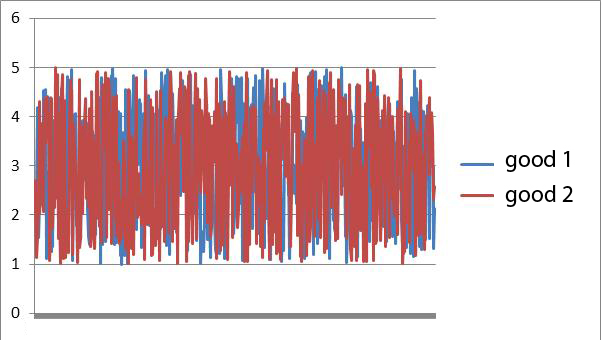
\includegraphics[width=0.4\textwidth]{ChapterTestingModels/Figures/CD_random1}}
\hspace{0.1}  
\subfloat[Income change for 2 Firms: none]{\label{fig:CDrand2}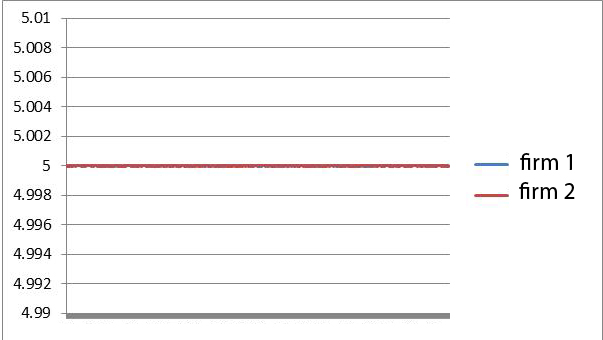
\includegraphics[width=0.4\textwidth]{ChapterTestingModels/Figures/CD_random2}}
\caption{2 Firms facing Cobb-Douglas demand randomise prices (\ref{fig:CDrand1}): no effect on either of their revenue (\ref{fig:CDrand2}). \label{fig:CD_2firm_randomPricing}}%
\end{figure}
\end{comment}

\begin{figure}[h!]
\centering
\subfloat[Optimal demand for good 1 (`opt1') and optimal demand for good 2 (`opt2'); Firm 2's optimal demand affected by its price changes. Firm 1's in unaffected: there are no elasticity effects.]{\label{fig:CDfix1}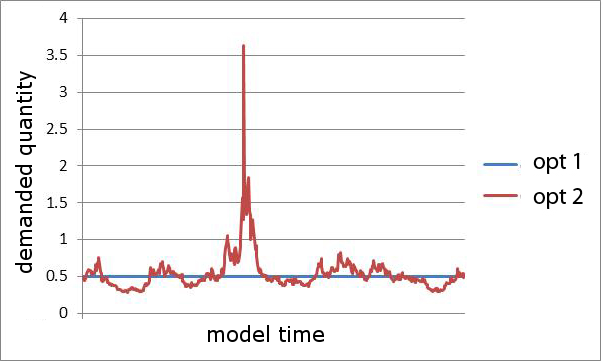
\includegraphics[width=0.7\textwidth]{ChapterTestingModels/Figures/CD_opt1edit2}}
\hspace{0.1}  
\subfloat[Price changes of Firm 2, underpinning changes in demand for good 2 (`opt2') in the previous figure.]{\label{fig:CDfix2}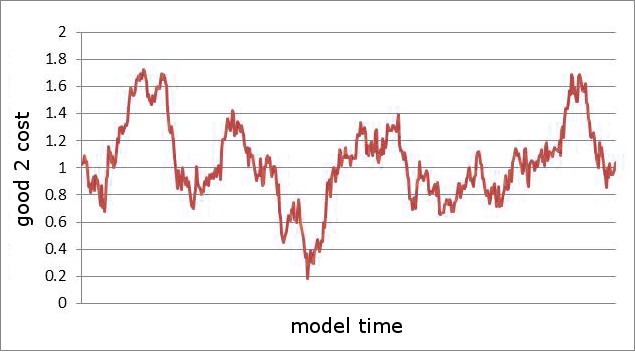
\includegraphics[width=0.7\textwidth]{ChapterTestingModels/Figures/CD_good2costedit}}
\caption{Two Firms selling goods 1 and 2: Firm 1's price fixed, 2 attempting to optimise price. Actors with Cobb Douglas utility: changing price of one has no effect on demand for the other. \label{fig:CD_1fixed}}%
\end{figure}

Figure \ref{fig:CD_1fixed} makes the same point with data from a model run: one firm's prices are fixed while the other attempts to find a revenue-maximising price. As mentioned above, this fails because they can affect no change on their revenue in this situation. For the fixed-price firm, actors consume a constant amount - and that is not altered by changes in the price of the other good. This shows that if People have a Cobb Douglas utility function in the model framework, demand for each good is independent of the other: there are no elasticity effects between them.

Note that, in situations where distance costs `melt away' or total model revenue has any other leak-points, the above would not hold: Firms could, for instance, improve their revenue by increasing proximity to their market, if expenditure on distance costs went elsewhere.

An interesting point arises from implementing the Cobb Douglas in agent form. Imagine a situation where only the agent-based approach to testing the utility function existed. Eventually, the independence of the two sectors in the Cobb Douglas would become apparent. But how would one be able to `explain' it? It is hard to imagine any answer that would not eventually reduce to the analytic result from the Lagrangian optimisation. By clearly showing, in a mathematical form, that $p_F$ and $p_M$ only appear in the demand equations for the same good, Equations \eqref{eq:optCDF} and \eqref{eq:optCDM} demonstrate that Cobb Douglas demand must always be entirely separate for the two goods. This is perhaps the best possible explanation; a cleanly analytic solution that the murkier agent approach makes more difficult to discern. Conversely, it is clear that Cobb Douglas utility \emph{imposes} this strict unit elasticity on sectors. As with the \gls{coremodel} this may be desirable, but it underscores the interdependence between Firms and People discussed in section \ref{sec:decstruct}. This is not necessarily an argument against \gls{abm}, since - as the rest of the chapter discusses - the flexibility of the method has other advantages. But it does highlight that, for many problems, neither method has a unique claim to explanatory power.

%What else to say about the Cobb Douglas? Come back and stick in an example of externalities for space costs, problems for 'general' analysis.
\subsection{Hill-climber versus constrained utility \label{sec:greedyvsconstrained}}

Chapter \ref{chapter:ABM} argued that utility is a useful concept for describing how people react to cost changes. In the model framework, two different approaches are tested for modelling People's utility: a `hill-climber' algorithm (see section \ref{sec:optimisingbundles}) and a more economically traditional constrained utility function, of the type outlined in section \ref{sec:constrained}.

What might be the problem in using constrained utility in an agent model? Section \ref{sec:rationality} pointed out that constrained utility is, as Leijonhufvud noted, ``a statement about actual performance, not just motivation''. The constrained function takes in a budget amount and goods prices and outputs an amount of demanded good. But what if the demanded good is not available? An `objective function' of this sort appears unable to deal with this situation. Consider the equation \eqref{eq:CESconstrained}, the constrained optima for an $n$-good \gls{ces} function described in section \ref{sec:constrained}. For a Person with a bundle of detected goods, the optimal amount for each good $c_j$ is given by:

\begin{equation}
c_j = \frac{p_j^\frac{1}{\rho-1}Y}{\sum_{i=1}^{n}p_i^\frac{\rho}{\rho-1}} \label{eq:CESconstrained2}
\end{equation}

 - where $p_j$ is the price of good $c_j$, $Y$ is the budget, and the denominator sums the price of each good raised to $\rho/\rho-1$. What happens in a situation where, for example, $c_1 = 1$ but only $0.5$ is available? There is then a different problem to solve: what is the optimal amount for the other goods, given that we know the available stock of  $c_1 = 0.5$. The constrained optima from equation \eqref{eq:CESconstrained} provides only demand as an output. There is no way to include a set demand amount for one or any of the goods; the function is simply not set up that way, and cannot be due to its roots in constrained optimisation. Neither is it quite as easy as removing $c_1$ from the list and recalculating, since demand for each affects all the others.

On the surface, the hill-climber algorithm approach appears a more plausible approach to utility: People weigh up a given mix of goods, and compare until they find what makes them `happiest' (that is, what gives them the highest utility). They do not have a superhuman constrained function informing them of their optimal demand. If any good is not available in the quantities they want, budget slices can be reassigned to the pot for the next iteration. In practice, however, this literal approach to stock consumption is complex to implement - not from the demand side, but because Firms then need to find some way to produce the \emph{correct} amount of stock given demand signals.

Fowler's approach is to make a tactical modelling choice that avoids the need to consider rationing of limited goods: ``workers select their optimal bundle of goods without reference to the actual supply of the good'' (\citealt{fowler_finding_2011} p.10). Thus, they still have an `objective' demand level. He notes a key informational advantage: this sends ``clear signals to firms about the actual level of demand for their goods at the current price'' (ibid.) As he says, it also avoids having to work out any explicit rationing strategy if several actors are competing for limited goods. 

While this is an effective simplification, it may be problematic depending on what the goal is. For instance, what exactly does it mean for Firms to receive demand signals for goods that People could not actually acquire? This is saying, `I wanted more than was available', and so in theory a Firm can use that information to inform their production decisions. This is a feasible approach if stock is theorised in a particular way; chapter \ref{chapter:connectedModels} presents a model that does this.

On a more mundane level, however, it is useful to compare the hill-climber algorithm to its constrained counterpart, to show that the two produce almost identical results. They are only different to the extent that the hill-climber algorithm cannot avoid a certain quantity of noise. Noise in utility is also put to good use in the model presented in section \ref{sec:firmsLoV} to examine how it impacts on Firms' ability to make appropriate decisions. The next section looks at the two approaches to utility maximisation in more detail.
%Section \ref{sec:optimisingbundles} explained that People assemble a set number of `Bundles' of goods, and work out the utility for each. They then select the highest utility bundle. 
 %I think. Better work out if that works. 
%There is, however, the problem of `objective demand' in a world that may not have the stock to meet it. One way to address this is to allow a Person to work with the stock that \emph{is} available. This can be done using the `hill-climber algorithm' approach...
\subsubsection{Comparing the two}

%In model runs, they produce almost identical results. Figure \ref{fig:GreedyVsConstrained} shows both the constrained and hill-climber algorithms optimising two and eight goods as distance costs are increased. Sub-figure \ref{fig:gnc5} compares the difference in utility levels: the hill-climber algorithm does not quite match the accuracy of the constrained, but gets very close.
%\cmt{Greedy: rewrite to take account of removed figure.}
How do the two approaches compare when stock levels are not an issue? The exact level of difference between the constrained optima and the hill-climber algorithm depends on the number of iterations the latter is given to ratchet towards utility-improving budget slices. Figure \ref{fig:GreedyItes} shows what difference the iteration number makes for two scenarios. Both show aggregate statistics for a thousand optimisations at each iteration-number point, up to 2000. Again, it is a \gls{ces} function at $\rho=0.5$, all good costs are even and the budget is one. This means the `correct' optima for each separate good is known. For the first example (\ref{fig:gi1} and \ref{fig:gi2}) optimising two goods, that is 0.5 for each, and as expected the constrained method finds this. Very low iteration numbers do not, on average, manage to get very close to this optimum, but by the time 1000 iterations are used, it is missing the perfect optima only minimally. Sub-figure \ref{fig:gi2}, however, shows that further improvements - though tiny, note the y-axis values - do continue to be made for iteration increases up to 2000 (in this example). There is always a little noise left in comparison to the constrained method.

The last sub-figure (\ref{fig:gi3}) shows the same outcome if eight goods are used - again showing results for one of those goods, whose analytic optima is 0.125. It is a quirk of the method that a higher number of goods can be optimised more quickly. The basis for this is an effect from good number: budget slices are all individually smaller: there is simply less scope for large variation due to the randomisation method used.

\begin{comment}
\begin{figure}[h!]
  \centering
  \subfloat[]  {\label{fig:gnc1}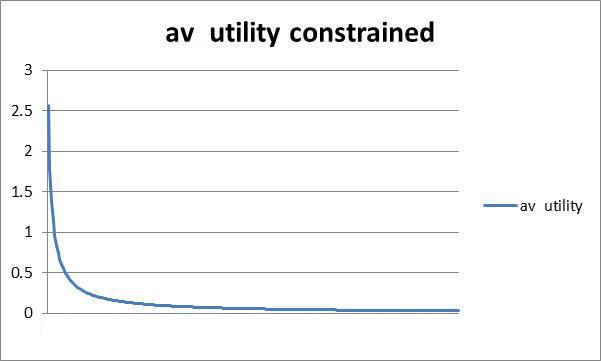
\includegraphics[width=0.4\textwidth]{ChapterTestingModels/Figures/avUtilityConstrainedcopy}}
  \hspace{0.1}    
  \subfloat[]  {\label{fig:gnc2}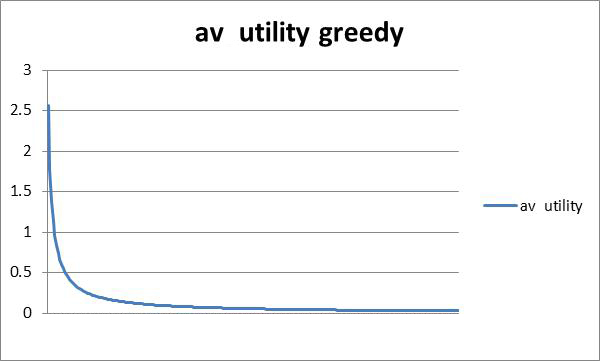
\includegraphics[width=0.4\textwidth]{ChapterTestingModels/Figures/avUtilityGreedycopy}}
  \hspace{0.1}    
  \subfloat[]  {\label{fig:gnc3}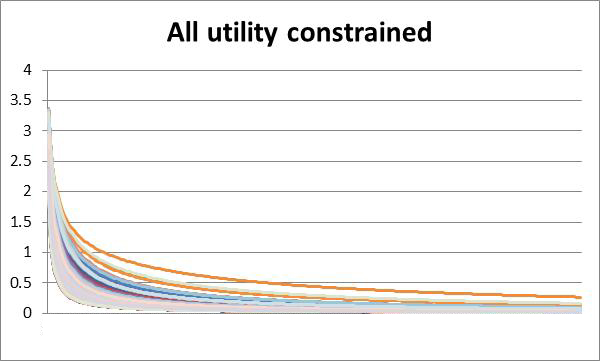
\includegraphics[width=0.4\textwidth]{ChapterTestingModels/Figures/allUtilityConstrainedcopy}}
  \hspace{0.1}    
  \subfloat[]  {\label{fig:gnc4}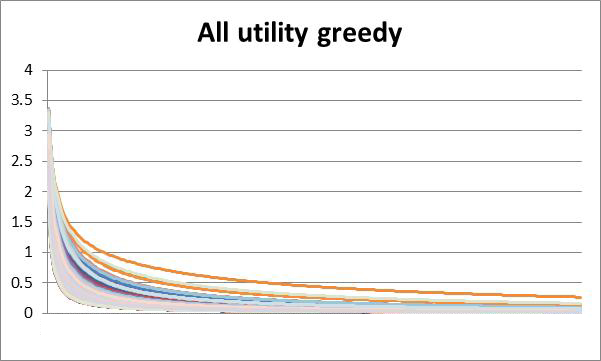
\includegraphics[width=0.4\textwidth]{ChapterTestingModels/Figures/allUtilityGreedycopy}}
  \hspace{0.1}    
  \subfloat[Difference between hill-climber (G) and constrained (C)]  {\label{fig:gnc5}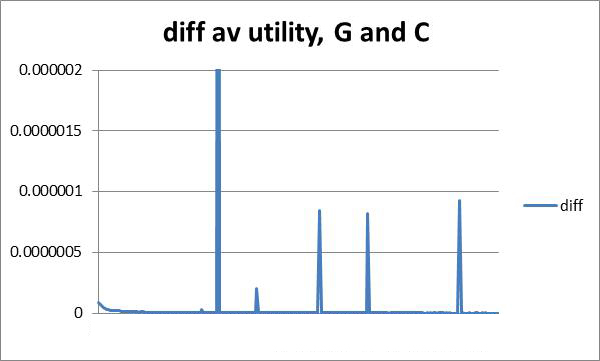
\includegraphics[width=0.4\textwidth]{ChapterTestingModels/Figures/diffAvUtilGnCcopy}}
  %\hspace{0.1}    
  \caption{Comparing hill-climber and constrained utility algorithms, fixed People, fixed Firms supplying goods at random distances at give a spread of values. Space costs on all goods increased from left to right. \label{fig:GreedyVsConstrained}}
\end{figure}
\end{comment}

\begin{figure}[p]
  \centering
  \subfloat[1 of 2 goods, zero to 2000 iterations]  {\label{fig:gi1}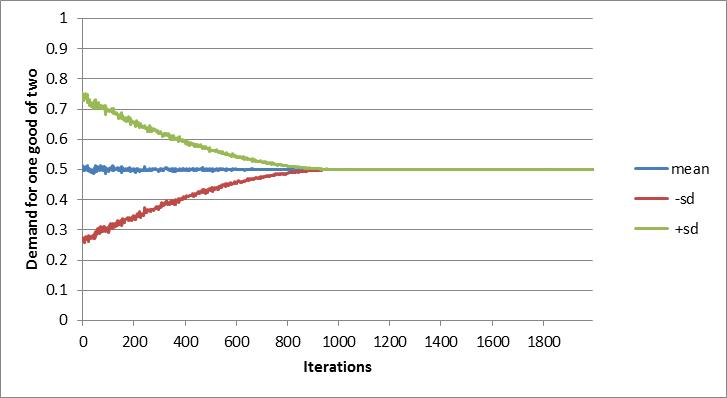
\includegraphics[width=0.8\textwidth]{ChapterTestingModels/Figures/greedyites1}}
  \hspace{0.1}    
  \subfloat[1 of 2 goods from 1100 iterations]  {\label{fig:gi2}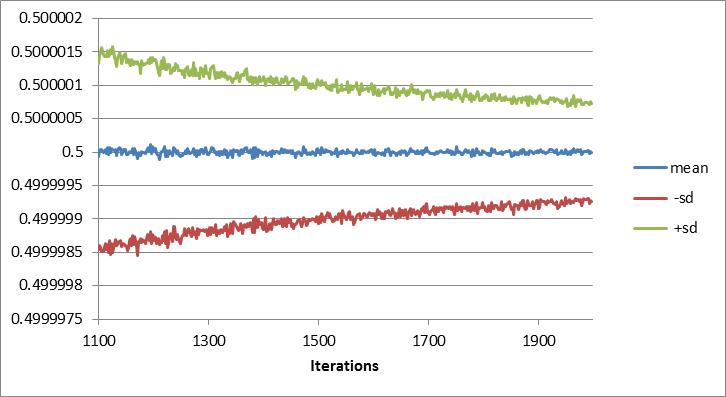
\includegraphics[width=0.8\textwidth]{ChapterTestingModels/Figures/greedyites2}}
  \hspace{0.1}    
  \subfloat[1 of 8 goods, zero to 2000 iterations]  {\label{fig:gi3}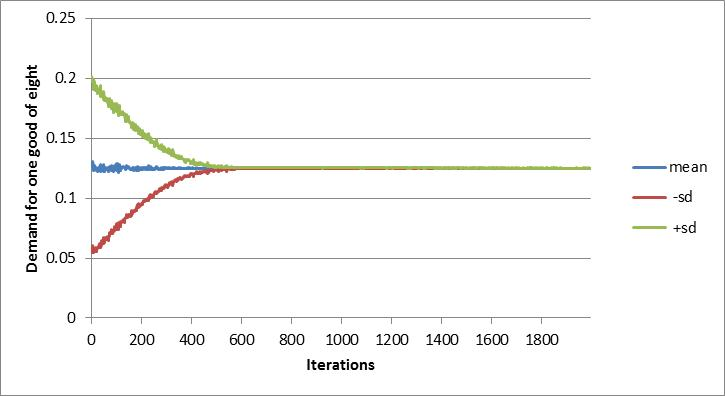
\includegraphics[width=0.8\textwidth]{ChapterTestingModels/Figures/greedyites3}}
  \caption{Hill-climber algorithm optimising 2 goods (\ref{fig:gi1} and \ref{fig:gi2}) and 8 goods (\ref{fig:gi3}). Optimum for one good is shown. 1000 optimisations for each iteration point, mean and one standard deviation.  \label{fig:GreedyItes}}
\end{figure}

The difference between the hill-climber and constrained algorithm is a useful way for thinking about the issue of realism and descriptive mapping in model structures, and the use of analytic optimisation more generally. Chapter \ref{chapter:ABM} discussed the centrality of equilibrium to neoclassical economic analysis, and the criticisms of agent modellers. Equilibrium skips to the end-point of a process: what about the process itself? 

Compare the underlying method of constrained versus hill-climber approaches to utility. Section \ref{sec:constrained} explained that the process of acquiring the constrained utility equations is to put them through a Lagrangian optimisation, where an algebraic budget is used to constrain the raw utility function. This effectively ditches the original utility and budget functions and replaces them with a third set of equations able to give optimal good quantities from an actual budget value and a set of good prices. In the model framework, as section \ref{sec:optimisingbundles} explained, those constrained equations work well since individual Good costs and People's budgets can be passed in, and optimal quantities of good returned. 

Once those values are found, however, the Person's utility level is still unknown. In terms of realism, this is a somewhat `spooky' outcome: the Person has their optimal quantities but does not know how happy it makes them. To get that information out of the model, the optimal good quantities must be fed \emph{back through} the original utility function. Causally, that makes no sense: a Person uses some function to find the good quantities they want, and then works out precisely how well off it makes them \emph{after} they have identified their optimal bundle.

In contrast, the hill-climber algorithm seems more `plausible', and certainly coheres more to the real-world process of decision-making. People must `hold up' bundles of goods and test the utility of each. Yet the hill-climber and constrained approach are clearly producing the same result, both succeeding at homing in on the point where the function can no longer change. However, the analytic constrained utility does the job better at a fraction of the computational expense - despite being causally muddled. This does not mean the hill-climber approach has no merit, but rather that the analytic method applied in this agent model served its purpose very well. 

In summary, both algorithms can find optimal utility levels, but the hill-climber algorithm has a processing overhead and noise. For most purposes in this thesis, the constrained approach was better. The difference between the two is no guide in that respect: as Friedman says, `everything depends on the problem'. 

However, the hill-climber algorithm does provide potentially useful flexibility for testing utility. For a start, it does not care about the form of utility it deals with. It takes a sample of good amounts as input: any and all object-oriented and algorithmic methods could then be applied to return a utility level. This could, for instance, allow interaction of tastes between actors as well as evolutionary approaches. (Though note, the particular hill-climb approach used here may not be suitable for situations with many local optima.)

The next section introduces a spatial cost element into the utility functions tested above.

\section{Two basic distance tests \label{sec:spacepoints}}

\subsection{Love of variety's interaction with distance \label{sec:utilspace}}
%\subsection{CES function \label{sec:cesspace}}

%\subsection{Spatial impact of the CES variables}

Section \ref{sec:CESbasics} explained that, if good prices are all equal, they will each be demanded in equal quantities when People are using a \gls{ces} function. This even split does not change for $0<\rho<1$ (where $\rho$ is the \gls{lov} parameter). The utility level \emph{derived} from the consumption of that even split increases inversely to $\rho$, but not the amount of each good demanded.

\begin{figure}[p]
  \centering
  \subfloat[No distance costs]  {\label{fig:cessp1}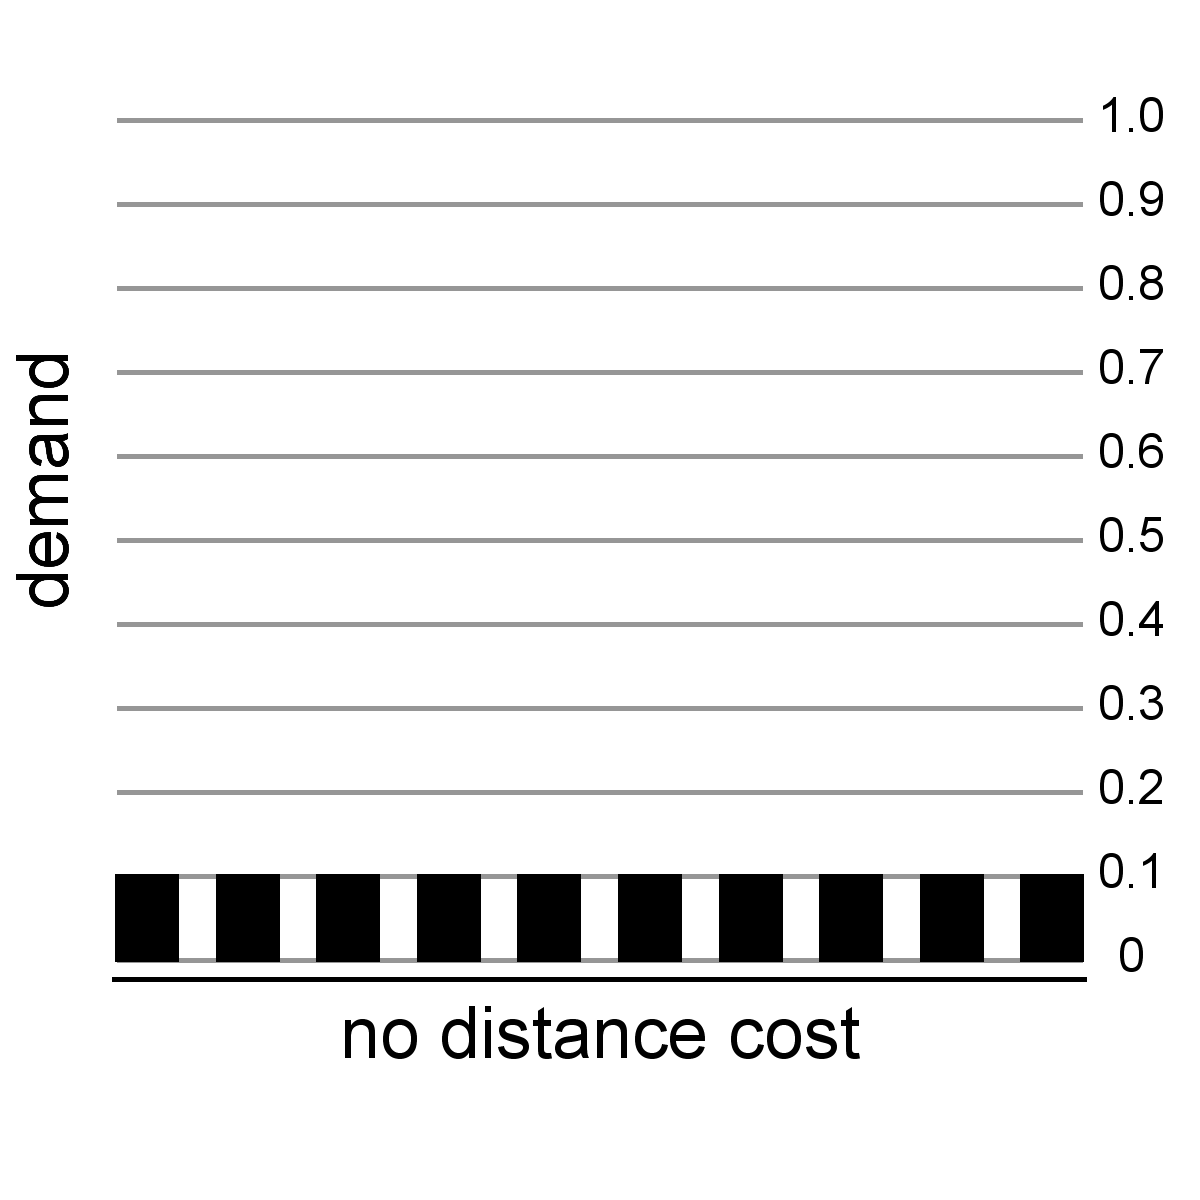
\includegraphics[width=0.49\textwidth]{ChapterTestingModels/Figures/JK_modelday_160_CESTest1Person9Firms_Wed-May-22-12_32_36-BST-2013__MainViz}}
  \hspace{0.1}    
  \subfloat[$\rho=0.8$]  {\label{fig:cessp2}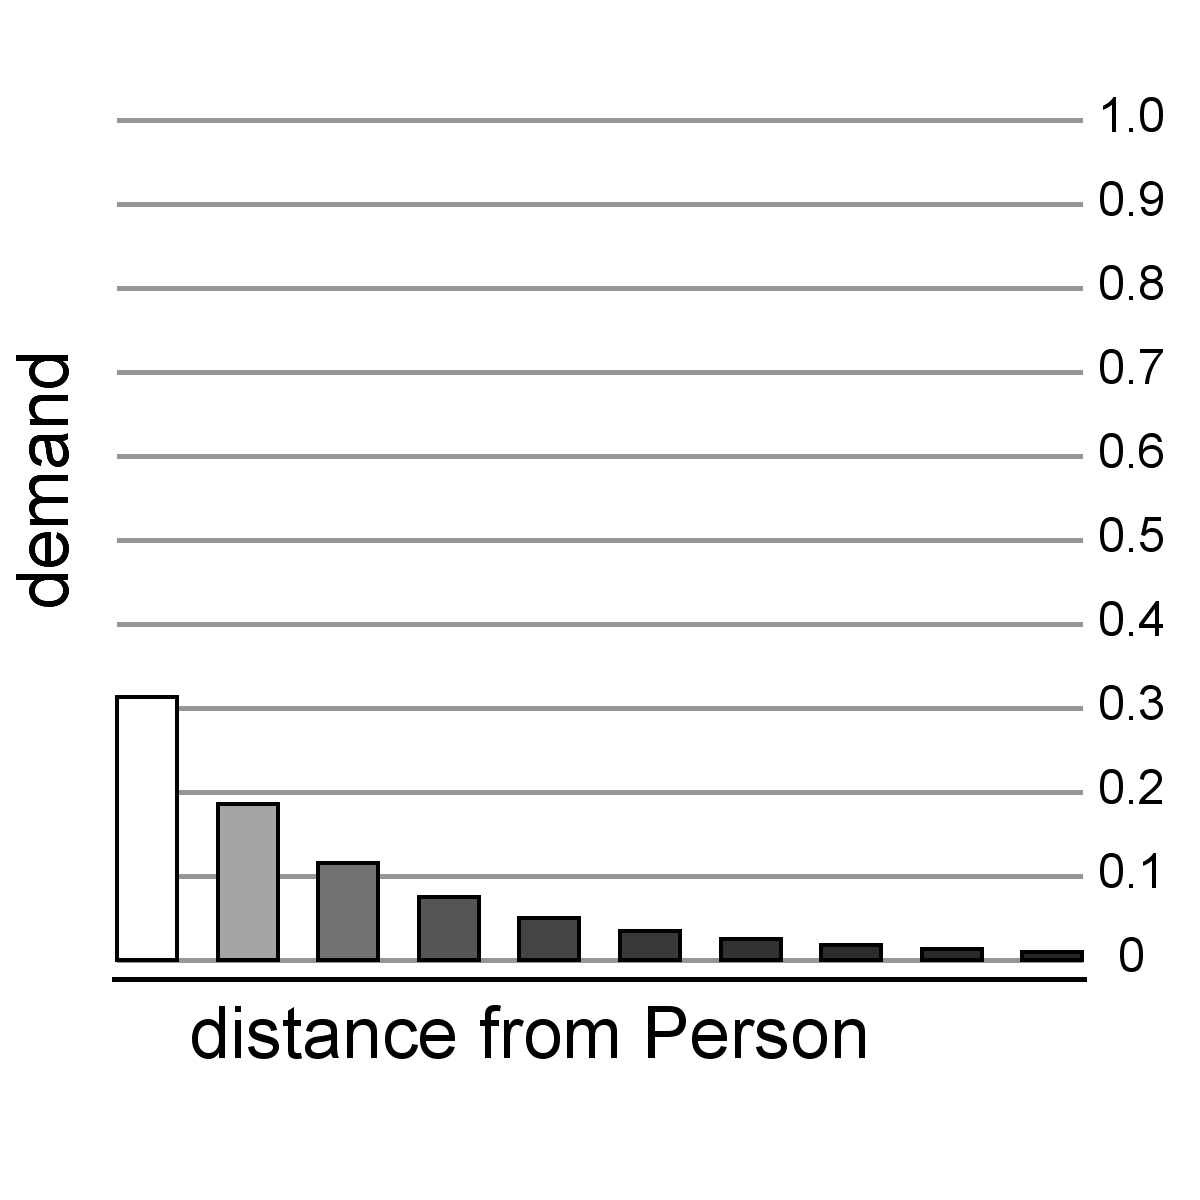
\includegraphics[width=0.49\textwidth]{ChapterTestingModels/Figures/JM_modelday_4386_CESTest1Person9Firms_Wed-May-22-12_34_17-BST-2013__rho0point8edit}}
  \hspace{0.1}    
  \subfloat[$\rho=0.9$]  {\label{fig:cessp3}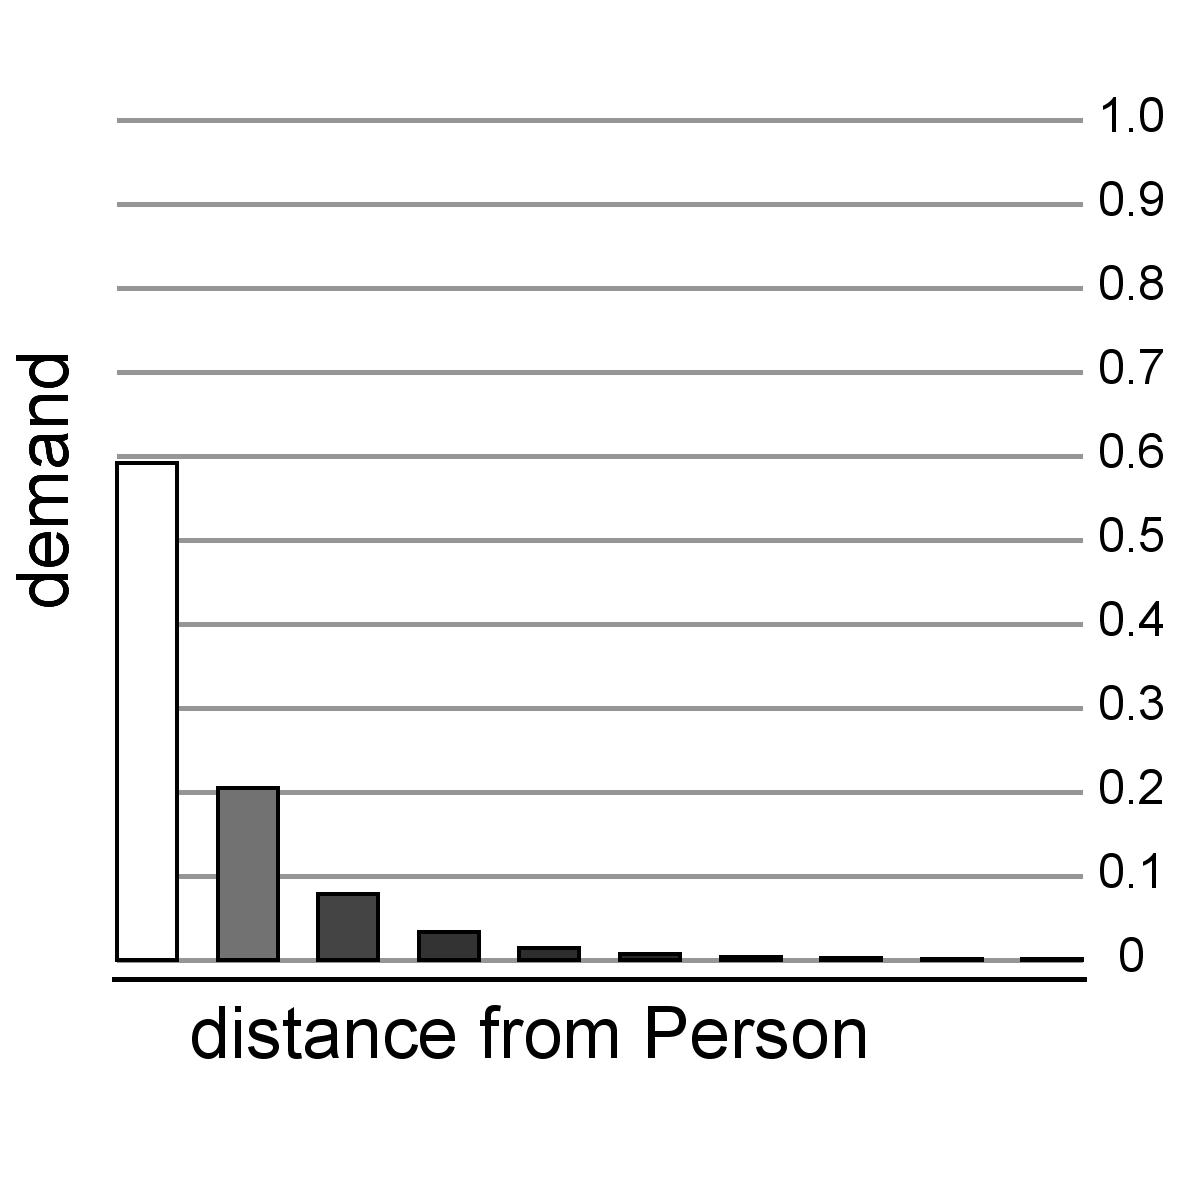
\includegraphics[width=0.49\textwidth]{ChapterTestingModels/Figures/JN_modelday_9419_CESTest1Person9Firms_Wed-May-22-12_34_56-BST-2013__rho0point9edit}}
    \hspace{0.1}    
  \subfloat[$\rho=1$]  {\label{fig:cessp4}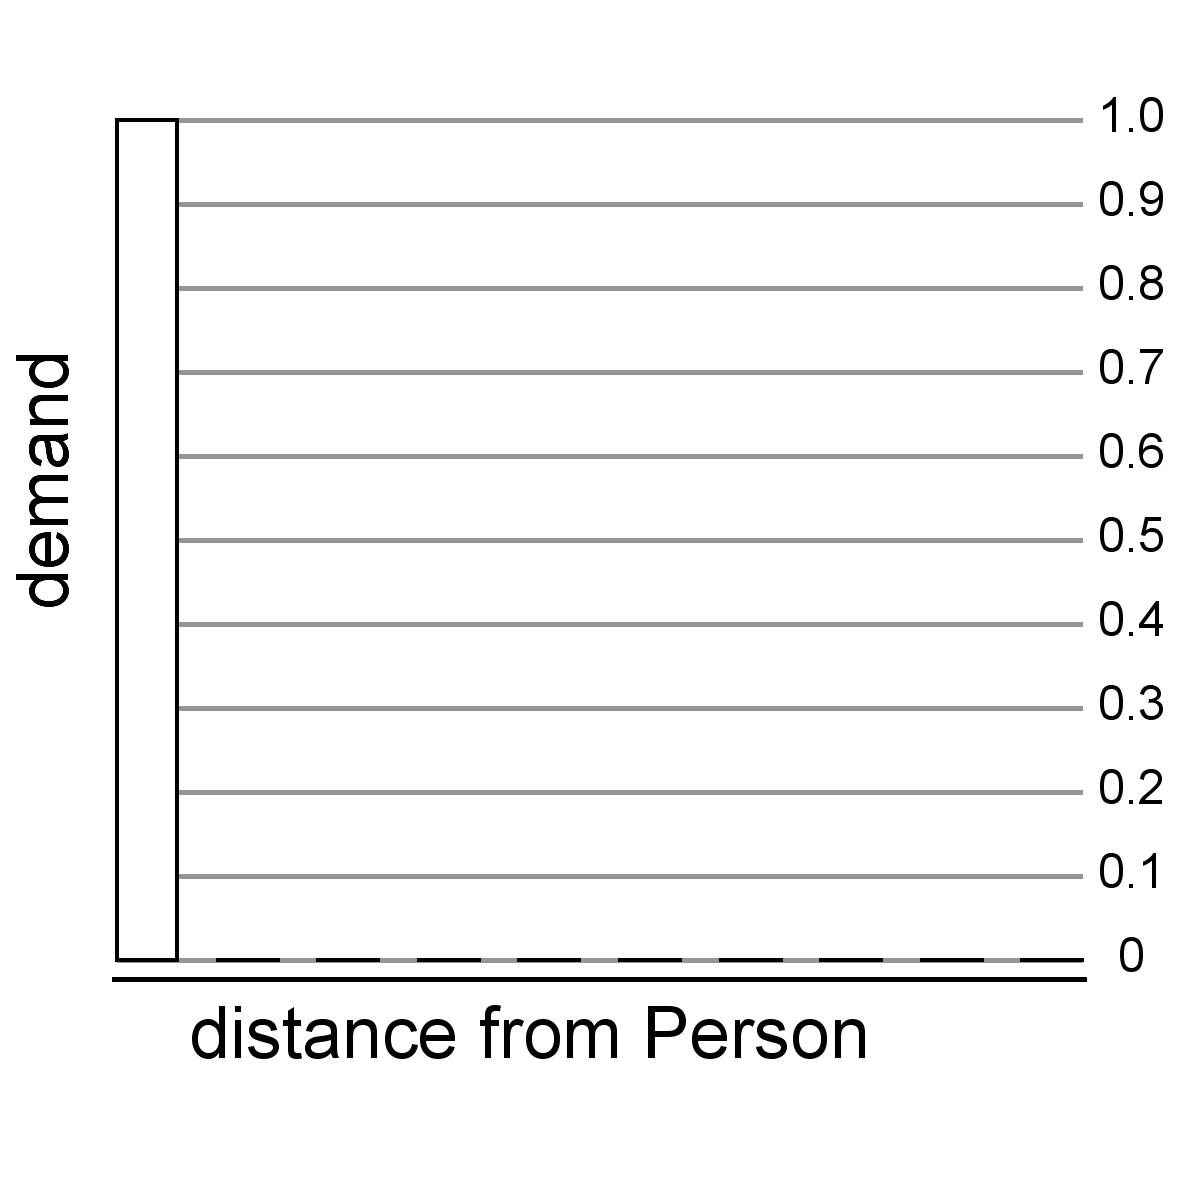
\includegraphics[width=0.49\textwidth]{ChapterTestingModels/Figures/JO_modelday_11994_CESTest1Person9Firms_Wed-May-22-12_35_15-BST-2013__rho1edit}}
  \caption{Effect on demand of changing $\rho$ in the presence of distance costs. Ten Firms are spread along the x axis evenly in distances of zero to one from a single Person. The Person is at the left origin of the x axis. Good cost and wage are $=1$. No distance cost in first graph, so demand is even; for others, distance cost is $1$ and $\rho$ is varied. \label{fig:CESrhoSpace}}
\end{figure}

If prices vary across goods, however, so does demand across goods as $\rho$ changes. This is important spatially: even if the base good prices are the same, distance costs will have a different effect on demand depending on $\rho$. (This is the basis for the use of the \gls{ces} function as a spatial interaction tool, mentioned in section \ref{sec:hiddencosts}.)

There are two separate effects to consider: that of \gls{lov} itself, controlled by $\rho$, and how changing the cost of moving goods impacts on demand. The following examples consider a single Person with a fixed location and fixed budget, spending it on a number of Firms at different, evenly spaced distances along a line. This can only be an illustrative way of conveying the effect of variable changes for one partial situation. For instance, the exact number and location of Firms will be vital to outcomes; here only nine or ten are considered. 

Figure \ref{fig:CESrhoSpace} visualises the dynamic in a model run scenario. In this model run, a Person is fixed in one position at the far left and ten Firms charging the same base price are evenly spaced in fixed positions from it. In sub-figure \ref{fig:cessp1} there are no distance costs: thus all goods cost the same. In this situation, $\rho$ will have no effect on the difference in demand between goods: the budget is evenly split between them. Sub-figures \ref{fig:cessp2} to \ref{fig:cessp4} all have a positive distance cost and so the further a Firm is from the Person, the higher the cost. The three different values of $\rho$ give a different spatial demand outcome. As $\rho$ approaches one, demand shifts to nearer goods, until at $\rho=1$, goods are completely substitutable and - stock permitting - demand will be met by the nearest provider. 

Figure \ref{fig:CESrhoMain} shows the same thing analytically for ten Firms at distances between $0$ and $1$. Regardless of the distance of the nearest, it will end up getting the whole spend as $\rho\rightarrow1$.

\begin{figure}[h!]
  \centering
  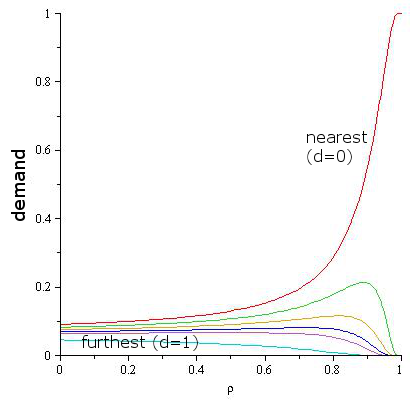
\includegraphics[width=0.7\textwidth]{ChapterTestingModels/Figures/CES_space_changeRhoeditedit}}
  \caption{Demand levels for ten goods spaced between a distance of zero and one, for $0<\rho<1$. Distance cost is $1$. One Person, $p=1$ and $c=1$, five nearest and one most distant shown here. As $\rho\rightarrow1$, the nearest good ends up getting the whole spend. \label{fig:CESrhoMain}}
\end{figure}

If the cost of moving goods across space is changed, the impact is not necessarily even for all Firms. This is due to the fact that, as those costs increase, demand for more distant goods is re-allocated to closer providers. This can lead to a `double dip' structure to demand: when space costs are low, demand will be even and nearer goods will sell equally to those more distant. As space costs increase, demand can increase for a time for the more proximate Firms. As costs rise, however, the overall cost effect will drive demand down again. Note, this is only the case for Firms \emph{nearby}: if a Person is at a distance of zero, demand will simply continue to increase as long as it is re-allocated from other goods. 

To illustrate, consider the following analytic example. The \gls{ces} constrained optimisation equation \eqref{eq:CESconstrained} can be used in a simplified form. Let $\rho=0.5$ and assume a budget of one. It then reduces to -

\begin{equation}
g_j = \left[P_j^2 \sum_{i=1}^{n} 1/P_i\right]^{-1}
\label{eq:CESsimpleForSpace}
\end{equation}

- Where $g_j$ is demand for good $j$, $P_j$ is its full price, and $P_i$ is the full price of goods $i$ through to $n$. The full price of each good is still just $p+(c\cdot d)$. Assuming the base good price to be the same for all goods ($p=1$), if no distance costs are present, a perfectly even mix will be the optimum. A series of goods at different distances from the buying Person will differ only in values for $d$ and how that multiplies the current value of per-unit space cost, $c$. In the following example, a number of goods are spaced at distances from either $0$ or $0.1$, up to a maximum distance of $1$. It is then possible to see the impact of changing the distance cost $c$. Using all these assumptions, the above equation becomes:

\begin{equation}
g_j = \left[(1+c\cdot d_j)^2 \sum_{d=0\ or \ 1}^{10} \frac{1}{1+c\cdot(d/10)}\right]^{-1}
\label{eq:CESsimpleForSpace}
\end{equation}

Here, a number of goods are spread out at different distances up to $1$. So: how do changes in the space-cost $c$ affect how demand is divided between the goods? Figure \ref{fig:CESrhoSpace2} shows the above equations analytically for $0<c<40$. Ten goods in total enter into the \gls{ces}, of which only the nearest five are shown here. Where the nearest is at $0.1$ (sub-figure \ref{fig:cesspp1}) the double-dip structure is apparent: re-allocated spend increases demand for that good before larger values of $c$ dominate. As mentioned above, whether there is a good available at distance $0$ makes a large difference. Sub-figure \ref{fig:cesspp2} shows that, if the nearest Firm is at $d=0$ - that is, if there is zero distance between consumer and producer - they receive all reallocated demand as distance costs increase for other Firms.

\begin{figure}[p]
  \centering
  \subfloat[Nearest Firm at $d=0.1$]{\label{fig:cesspp1}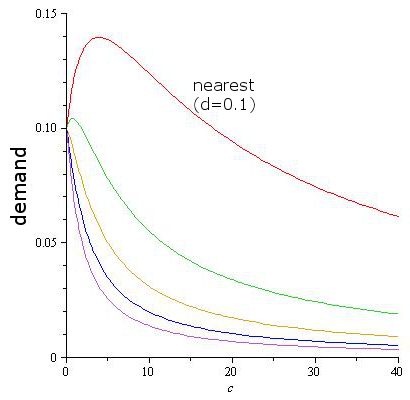
\includegraphics[width=0.68\textwidth]{ChapterTestingModels/Figures/CES_space_Rho_cchange1editedit}}
  \hspace{0.1}    
  \subfloat[Nearest Firm at $d=0$]{\label{fig:cesspp2}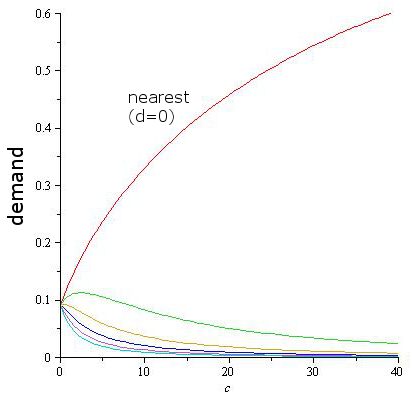
\includegraphics[width=0.68\textwidth]{ChapterTestingModels/Figures/CES_space_Rho_cchange2editedit}}
  \caption{Impact of changing good space cost: one Person, ten Firms. In figure \ref{fig:cesspp1} the nearest Firm is at a distance of $0.1$ from the Person; in figure \ref{fig:cesspp2} the nearest Firm is at $0$. Firms are spaced between zero or $0.1$ and one, with the five nearest shown here. Value of $c$ (cost of moving good a unit of distance) on x axis. Note: demand axes have different values. \ref{fig:cesspp2} shows Firm at $d=0$ receiving all re-allocated demand as distance costs increase, unaffected by distance cost change.  \label{fig:CESrhoSpace2}}
\end{figure}

%\cmt{Removed `location differences': just read to make sure no important points there. (It's in cuttinz.)}
%\cmt{Conclude LoV spatial basics section: this is what it does. So onward..}
\subsection{The `black hole' outcome \label{sec:blackholemodel}}


Space imposes costs and, like any other costs, actors will minimise them if they can. The most obvious spatial outcome is that all actors will simply remove those costs, collapsing to a point in the process, unless other forces mitigate against this. Such forces exist; one outcome of using them is discussed in the next section. But without them, does the model reproduce the basic `black hole' finding? In this model run, with all other costs fixed, Firms and People are allowed to find their preferred location using the methods described in chapter \ref{chapter:modelfw} - People comparing different Bundle locations and Firms using a feedback that crawls towards revenue-improving locations.

\begin{figure}[h!]
  \centering
  \subfloat[People]
  {\label{fig:bhg2}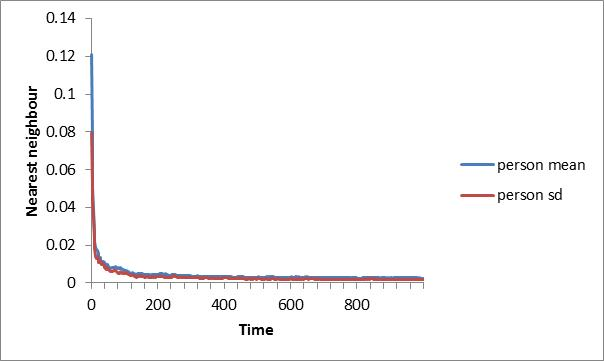
\includegraphics[width=0.7\textwidth]{ChapterFramework/figures/mnnd_blackhole_manyruns1}}
  \hspace{0.2}  
  \subfloat[Firms]{\label{fig:bhg3}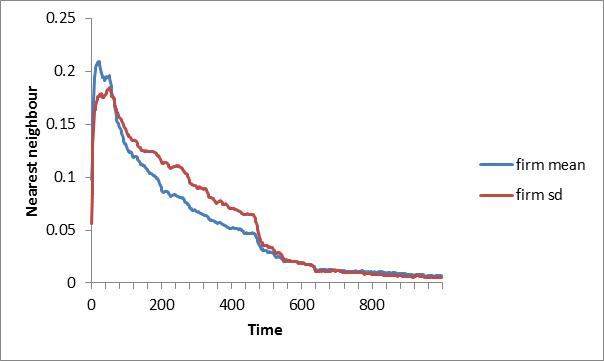
\includegraphics[width=0.7\textwidth]{ChapterFramework/figures/mnnd_blackhole_manyruns2}}
  \caption{Means and standard deviations of nearest neighbour distance, randomised starting locations, averaged from 20 model runs.  \label{fig:blackholegraphs}}
\end{figure}
%Data: location1/data/nearestneigh20runs

Figure \ref{fig:blackholegraphs} shows the outcome of this model run over a thousand days for twenty People and four Firms. The model was run twenty times with different random starting conditions; the data shows the average outcome. All actors converge on a point, incrementally seeking positions closer to each other to reduce space costs or, in Firms' case, increase revenue. People quickly converge, while Firms take much longer: this reflects the fact that Firms must use a feedback that cannot always be relied upon - section \ref{sec:firmsLoV} discusses this point in detail. Ultimately, all actors do reduce their space cost as close to zero as they can.

\section{Mobile People \label{sec:results}}

This section investigates the results of allowing People in the model to choose their location. For all but the last model in section \ref{sec:LoVresult}, a Firm or Firms are fixed at a single point and People organise themselves around that point, incurring density costs as they do so. The set-up for the models in this section is as follows:

\begin{itemize}
	\item An $R^2$ plane of distance $1$ per axis.
	\item $500$ People (unless otherwise stated) are mobile, able to select the Bundle with the optimal location as outlined in section \ref{sec:howPeopleAct}.
\item Firms have a fixed location. The number of Firms vary depending on the job the model is doing; see each section below for specifics. Base good costs are set to one; distance costs are varied for some model runs.
	\item People incur a `density cost' as outlined in section \ref{sec:densitycostsetupFramework}.
\end{itemize}

As explained in section \ref{sec:densitycostsetupFramework} the multiplication factor for the density cost is set to $10$ for all but one set of model runs, because it provides an incentive for People to trade density cost off against distance. Section \ref{sec:notutilityeq} discusses how increasing density cost higher impacts on spatial equilibrium assumptions. 

\subsection{Basic monocentric result: density cost traded off against distance \label{sec:typicalmodeloutput}}

\begin{figure}[p]
\centering
\subfloat[People in $R^2$ buying from central Firm. Larger/lighter squares indicate higher incurred density cost, rising towards the centre.]{\label{fig:densityviz}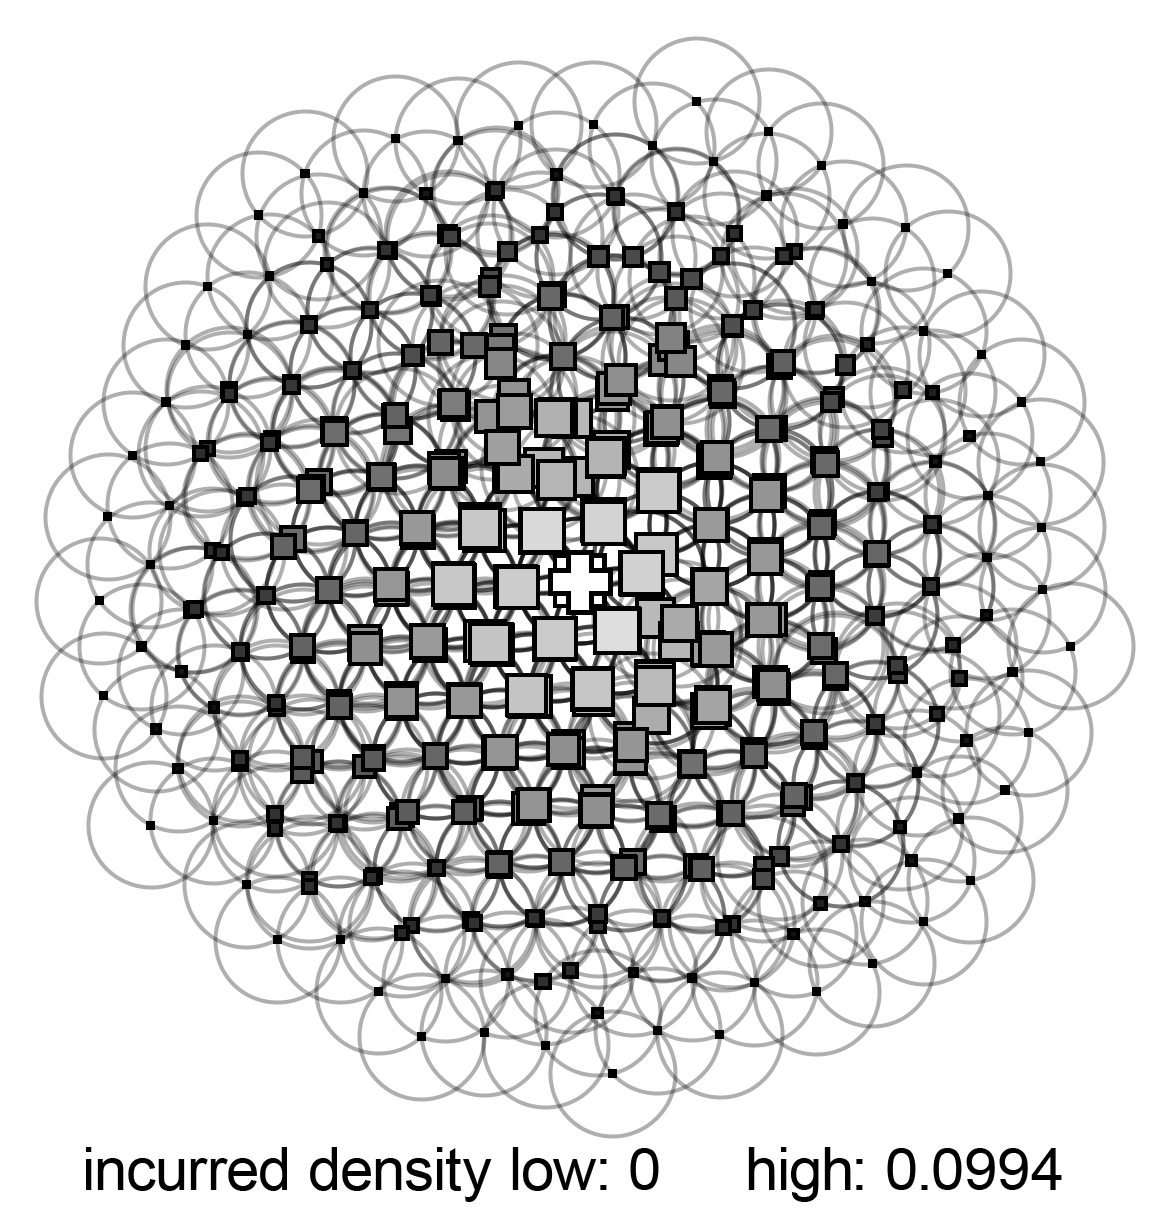
\includegraphics[width=0.6\textwidth]{ChapterTestingModels/Figures/IB_CEUS1_Mon-Dec-03-15_55_58-GMT-2012__MainVizDensitycopy}}%
\hspace{0.2}
\subfloat[Incurred density cost vs distance to centre for individual People]{\label{fig:densitygraph}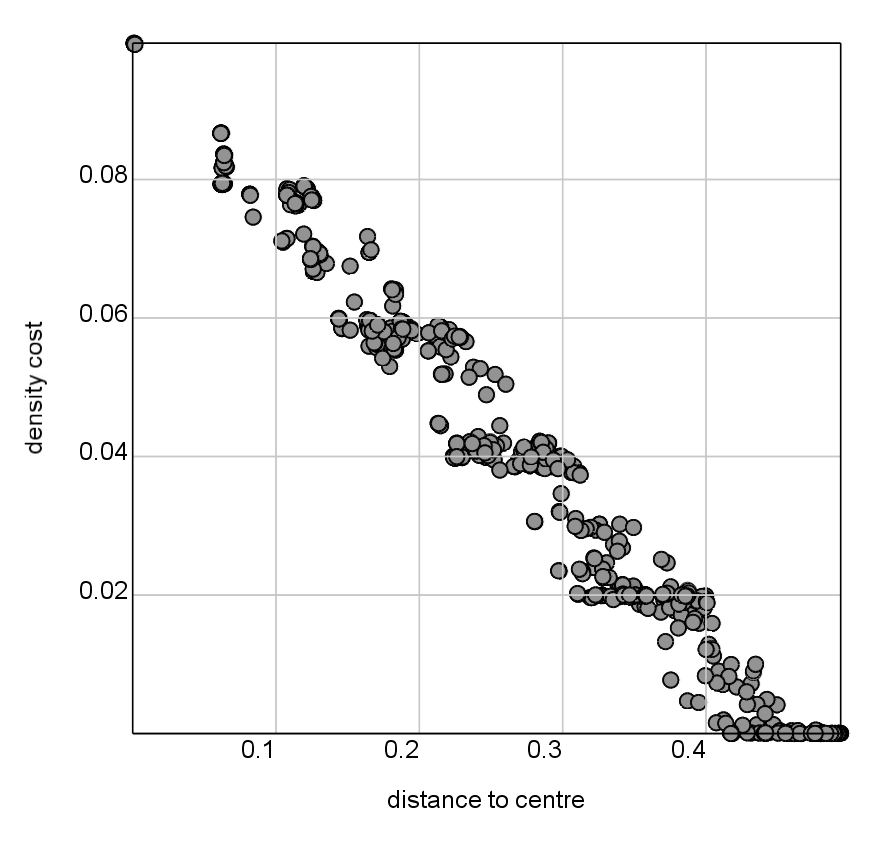
\includegraphics[width=0.7\textwidth]{ChapterTestingModels/Figures/ID_CEUS1_Mon-Dec-03-15_57_17-GMT-2012__distanceToCentralFirm_vs_chosenDensityCostcopy}}%
\caption{Model run: 500 People; density cost $=10$; distance cost $=0.25$; no commute cost. Correlation shows datapoints for individual People. \label{fig:sixresults}}%
\end{figure}

Figure \ref{fig:sixresults} provides an overview of the model's outputs from a typical monocentric setup. Sub-figure \ref{fig:densityviz} is a visualisation of People locating in an $R^2$ space; this style is used throughout this section. These visualisations use size and shade of squares to indicate the \textbf{relative} range of values during the iteration being shown. Small, black squares are the lowest value of the shown variable (in this case density cost); large, white squares are the highest. Sub-figure \ref{fig:densitygraph} shows the same information in a different way, showing each Person's distance to the central Firm on the x-axis versus the density cost they are incurring closer to the centre. 
%These are paired with graphs from the same iteration correlating each Person's distance to the central Firm with (respectively) utility (\ref{fig:utilitygraph}) and incurred density cost (\ref{fig:densitygraph}). 

Figure \ref{fig:utilityEqMonoUtility} is from the same model run. It is telling one clear story: utility is close to identical for all People (staying close to $0.9$) regardless of distance from the central Firm. Utility is equilibriating to an equal value for all People over distance. In figures \ref{fig:densityviz} and \ref{fig:densitygraph}, the density incurred by People is shown to drop off linearly over distance from the centre: a trade-off is being made between density and distance cost.  This lends support to the argument for assuming spatial equilibrium (section \ref{sec:litbits}). However, there are scenarios where this assumption (that spatial equilibrium is also a utility equilibrium) fails; see section \ref{sec:notutilityeq}.
%He also explains its power well: ``this core insight comes from the idea that if identical people are choosing to live in different places then those two different places must be offering an equivalent bundle of advantages'' (ibid). (\citeyear{glaeser_cities_2008} p.4)  

\begin{figure}[h]
\centering
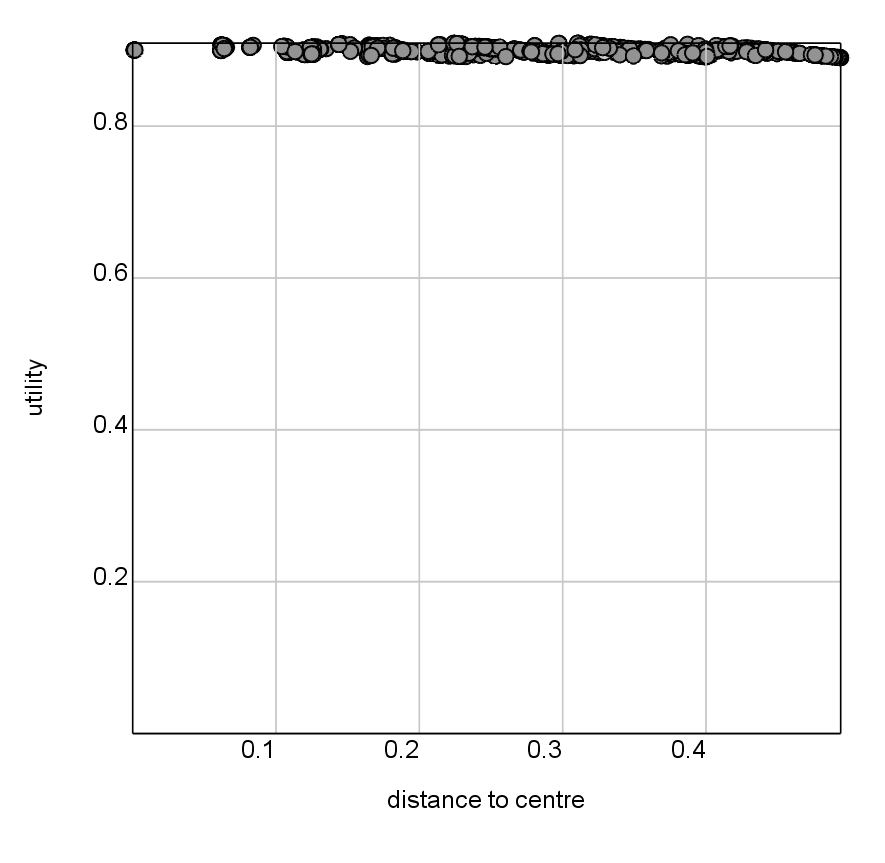
\includegraphics[width=0.7\textwidth]{ChapterTestingModels/Figures/IF_CEUS1_Mon-Dec-03-15_57_42-GMT-2012__distanceToCentralFirm_vs_maxUtilitycopy}}%
\caption{Utility vs distance to central Firm: utility equilibriates. 500 People; density cost $=10$; distance cost $=0.25$; no commute cost. \label{fig:utilityEqMonoUtility}}%
\end{figure}

Before section \ref{sec:notutilityeq}, the following analyses work within the range where density cost sets up a trade-off to explore exactly how it functions from agents' point of view.

\subsection{Density cost \label{sec:densitycostsetup}}

To further illustrate the effect of the density cost, figure \ref{fig:densityresult1} shows a typical result from People making this trade-off in a monocentric model with a single Firm at the centre. Light circles indicate the density cost radius for each Person. Darker circles show a random selection of People, including the position of others they are incurring a density cost from (the smaller white circles). The resulting hexagonal patterning is a striking feature of People's self-organising behaviour, resulting from minimising density cost by finding interstitial points. However, for the purposes of this thesis - as section \ref{sec:litbits} discussed - it is economically uninteresting. Sub-figure \ref{fig:densitygraphnumPeople} shows the discrete number of People entering into density cost calculations correlated to how far each Person is from the central Firm. Each circle represents an individual Person; they are willing to incur higher density costs towards the centre.

\begin{figure}
\centering
\subfloat[People in $R^2$ buying from central Firm. People (density cost radii shown) and Firm (white cross in centre). Random selection of People's density cost radii (thicker black circles) showing location of detected People entering into density cost calculation (small white circles).]{\label{fig:densityviz}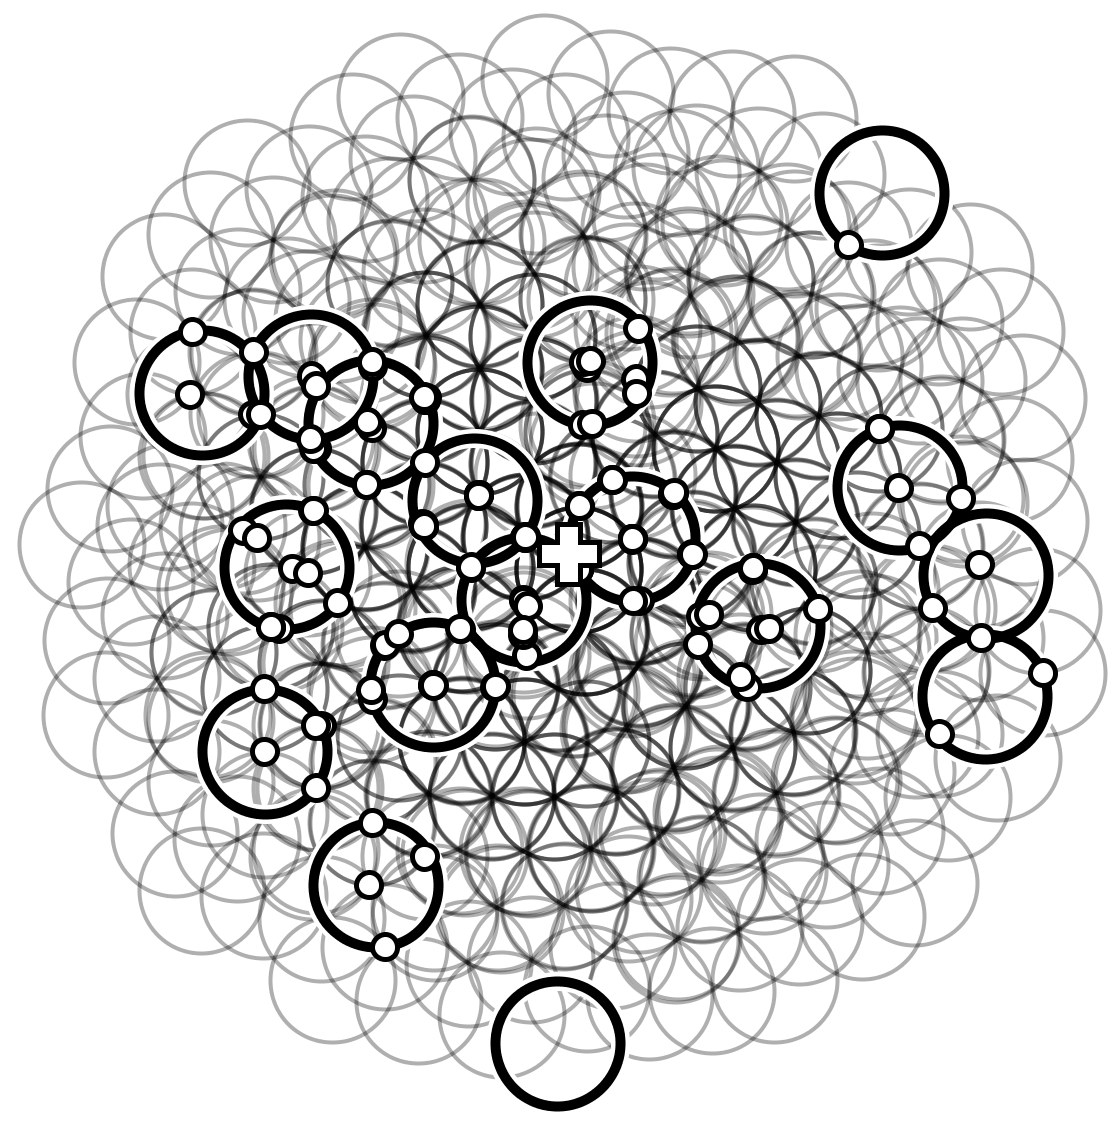
\includegraphics[width=0.6\textwidth]{ChapterTestingModels/Figures/SB_modelday_1397_CEUS1_Sat-Dec-15-17_24_49-GMT-2012__MainViz2}}%
\hspace{0.2} 
\subfloat[Number of People in each Person's density cost radius vs each Person's distance to central Firm. For each Person, discrete number of People entering into density cost calculation is shown on y axis. This increases with proximity to centre.]{\label{fig:densitygraphnumPeople}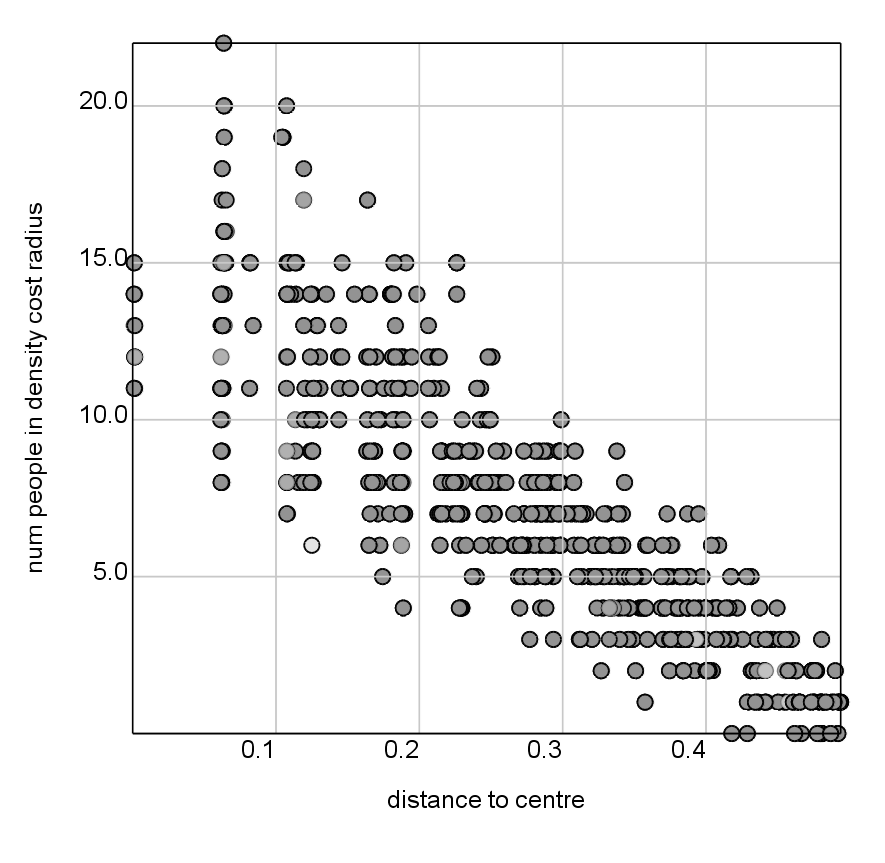
\includegraphics[width=0.7\textwidth]{ChapterTestingModels/Figures/IC_CEUS1_Mon-Dec-03-15_57_00-GMT-2012__distanceToCentralFirm_vs_numPeopleInDensityCostRadiuscopy}}%
\caption{Effect of density cost in a `monocentric' model run: 500 People; density cost $=10$; distance cost $=0.25$; no commute cost. People optimise in response to distance and Density cost. \label{fig:densityresult1}}%
\end{figure}

%Save any other spatial costs, a density cost by itself is, naturally, dispersive. The point of economic interest is how agents choose to trade that cost off against other benefits they find from choosing a particular location. Figure \ref{fig:densityresult1} shows a typical result from People making this trade-off in a monocentric model with a single Firm at the centre. Full details are given below; this example concentrates on illustrating the effect of the density cost. Light circles indicate the density cost range for each Person. Darker circles show a random selection of People, including the position of others they are incurring a density cost from (the smaller white circles). The resulting hexagonal patterning is a striking feature of People's self-organising behaviour, resulting from minimising density cost by finding interstitial points. However, for the purposes of this paper, it is economically uninteresting. Sub-figure \ref{fig:densitygraphnumPeople} shows the discrete number of People entering into density cost calculations correlated to how far each Person is from the central Firm. Each circle represents an individual Person; they are willing to incur higher density costs towards the centre.
\subsection{Impact of changing spatial and non-spatial costs on size of settlement \label{sec:spatialvsnon}}

\begin{figure}[]
\centering
\subfloat[]{\label{fig:spatialvsnon_wage}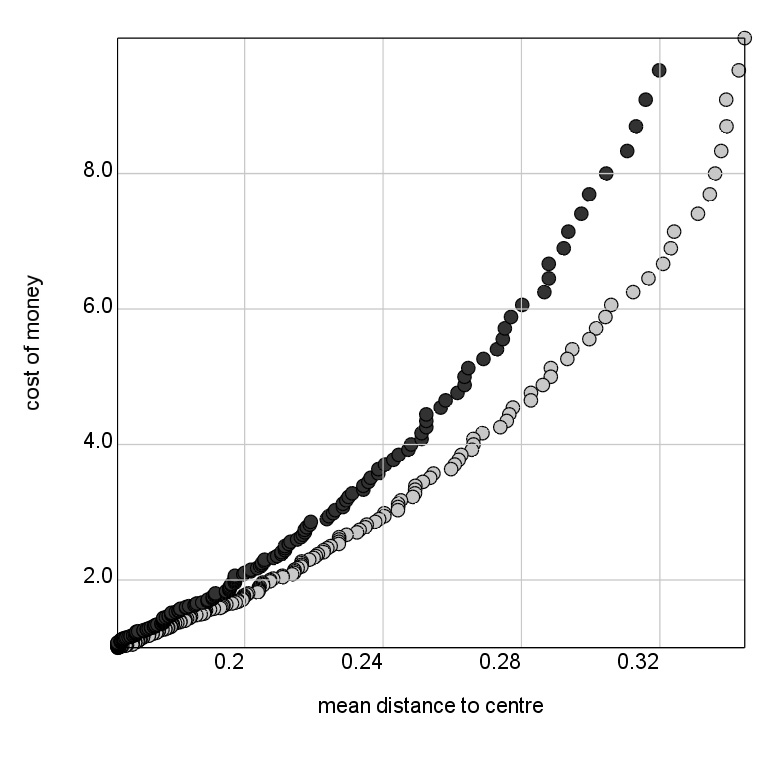
\includegraphics[width=0.7\textwidth]{ChapterTestingModels/Figures/distanceToCentralFirm_vs_wageOffer}}%
\hspace{0.2}  
\subfloat[]{\label{fig:spatialvsnon_commute}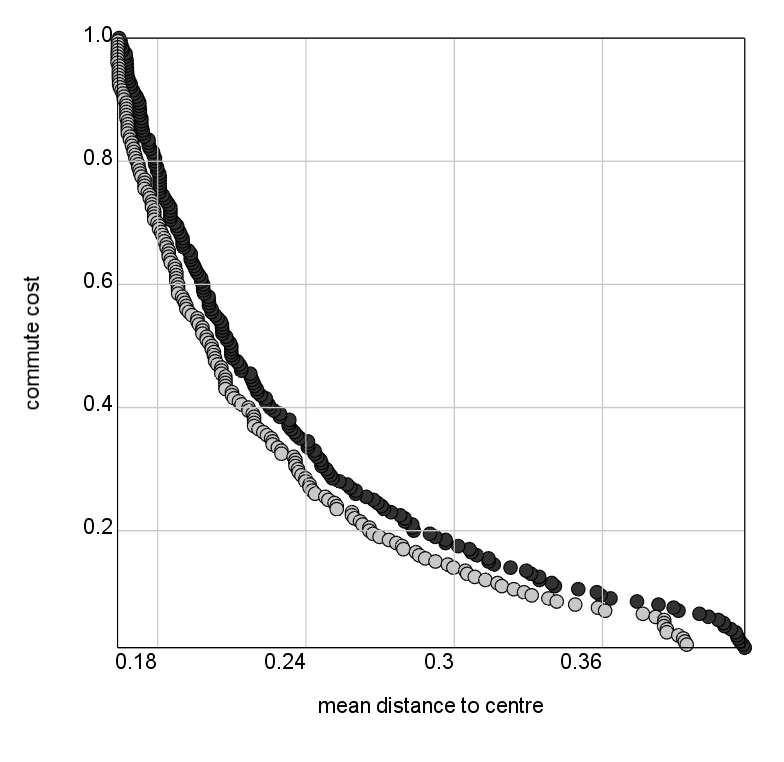
\includegraphics[width=0.7\textwidth]{ChapterTestingModels/Figures/distanceToCentralFirm_vs_COMMUTECOST}}%
\hspace{0.2}  
\caption{Wage offer (`cost of money') and commute cost versus mean distance to centre; single datapoint shown: average for all People, taken at spatial equilibrium. Each is parameter-swept (positive in black, negative in grey) in increments of $0.005$. `Spatial equilibrium' is assumed when mean agent movement $<0.0001$ average over $10$ iterations. \label{fig:spatialvsnon}}%
\end{figure}

\begin{figure}[]
\centering
\subfloat[]{\label{fig:spatialvsnon_good}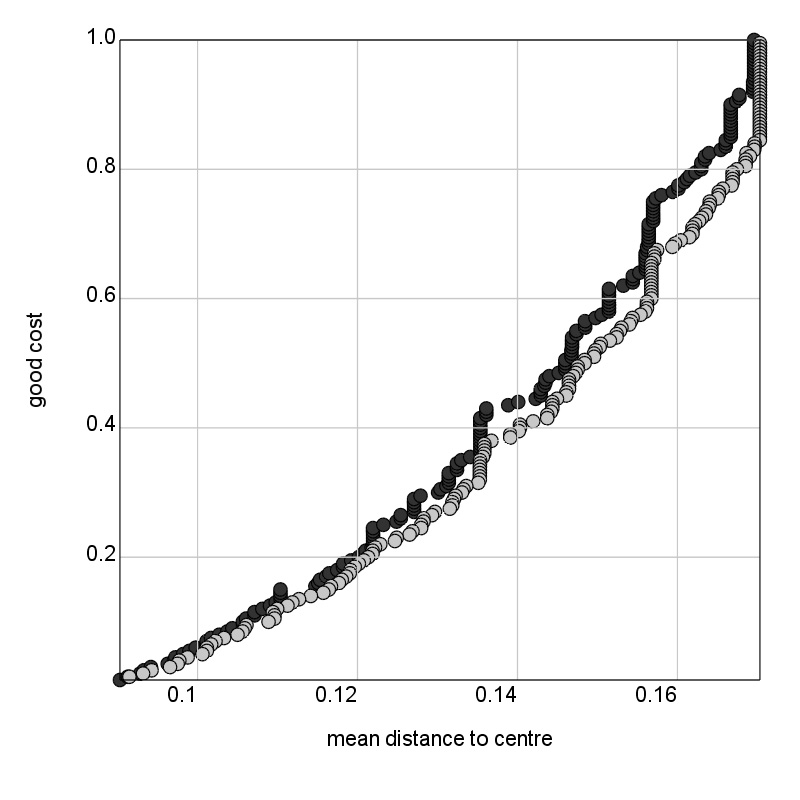
\includegraphics[width=0.7\textwidth]{ChapterTestingModels/Figures/distanceToCentralFirm_vs_goodCost}}%
\hspace{0.2}  
\subfloat[]{\label{fig:spatialvsnon_del}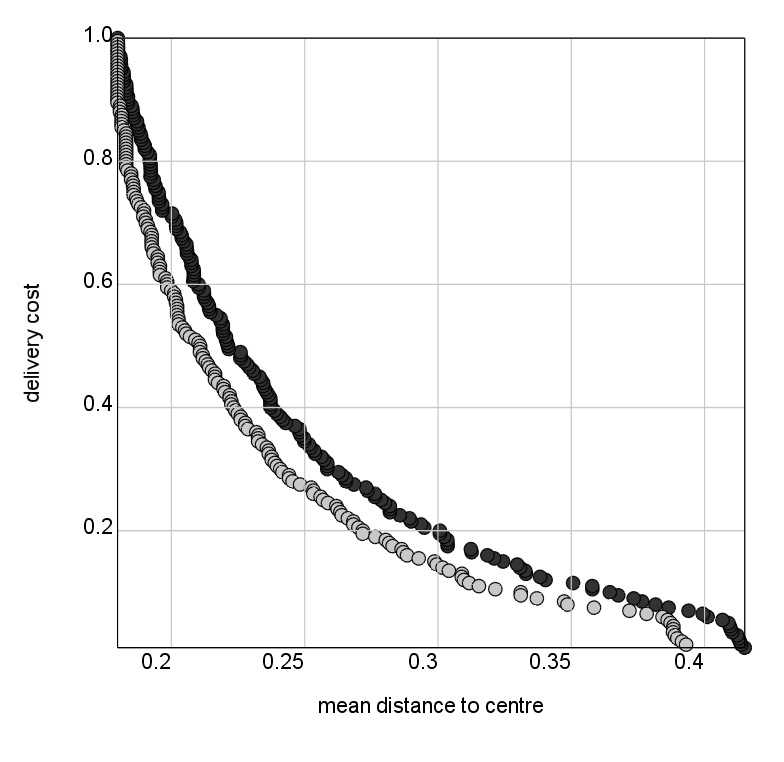
\includegraphics[width=0.7\textwidth]{ChapterTestingModels/Figures/distanceToCentralFirm_vs_deliveryCost}}%
\caption{Base good cost and distance cost versus mean distance to centre; single datapoint shown: average for all People, taken at spatial equilibrium. Each is parameter-swept (positive in black, negative in grey) in increments of $0.005$. `Spatial equilibrium' is assumed when mean agent movement $<0.0001$ average over $10$ iterations. \label{fig:spatialvsnon2}}%
\end{figure}

Section \ref{sec:reframingpeoplecost} explained that the cost of moving both people and goods can be broken down into spatial and non-spatial components. Figures \ref{fig:spatialvsnon} and \ref{fig:spatialvsnon2} show the result of sweeping each of these four costs: wage (reframed as base `cost of money' in time) and commute cost in figure \ref{fig:spatialvsnon} and base good cost versus distance cost in figure \ref{fig:spatialvsnon2}. The model setup is: $300$ People buy a Firm's single good and work for a fixed wage. Each of the four variables is changed from zero to one and from one back to zero in increments of $0.005$. Both directions are checked to highlight any hysteresis: darker circles indicate increasing distance, lighter circles decreasing. `Spatial equilibrium' is assumed when mean movement for all People drops below an average of $0.0001$ over ten iterations. A datapoint is taken when this condition is met. At least ten iterations are then allowed to pass before checking for stability again. The impact on spatial morphology  is measured using the mean distance of all People from the centre firm, which is larger as People spread further out from the centre. 

Sub-figures \ref{fig:spatialvsnon_wage} and \ref{fig:spatialvsnon_good} show the effect of varying the non-spatial costs. Changing both the `cost of money' and the good cost effectively alter the real wage, and both have a spatial impact due to their interaction with density cost. Increasing the real wage makes People more able to offset density cost: they agglomerate. Conversely, sub-figures \ref{fig:spatialvsnon_commute} and \ref{fig:spatialvsnon_del} show the effect of varying the spatial costs, changing the cost of moving goods and wage across space differently depending on a Person's location. Decreasing distance cost and commute cost have the same effect: goods and wages can get further for cheaper. While overall this increases Peoples' real wages, the spatial effect is opposite: they disperse. 

This equivalence of effect in the model framework is useful for conceptualising People buying goods with time directly in the `transmission belt' model (chapter \ref{chapter:connectedModels}).

\subsection{What drives agent location choice in the monocentric model? \label{sec:rationalchoices}}

\begin{figure}[p]
\centering
\subfloat[utility vs distance cost]
{\label{fig:discreteregiondelcost}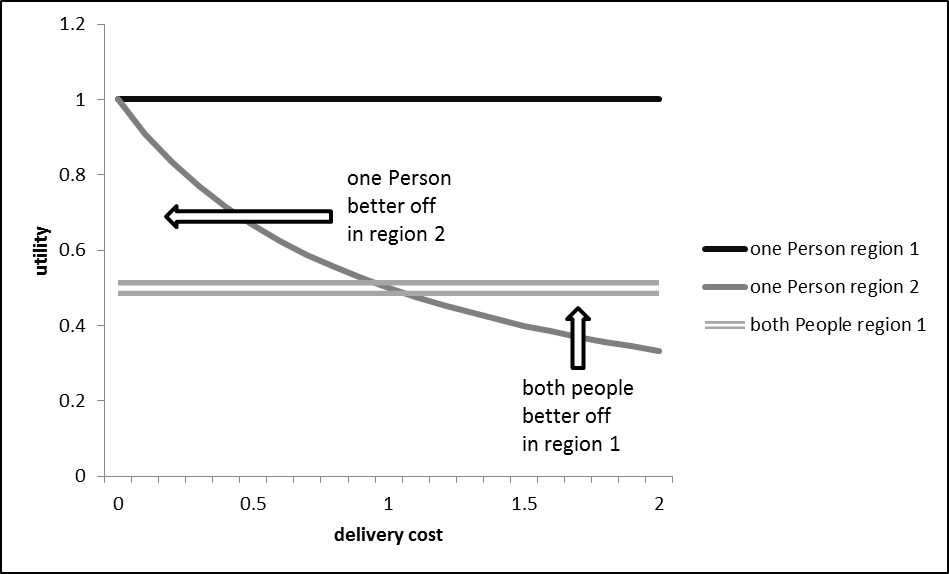
\includegraphics[width=0.9\textwidth]{ChapterTestingModels/Figures/2regionDiscreteDeliveryCostB&W}}%
\hspace{0.2}  
\subfloat[utility vs base good cost]{\label{fig:discreteregiongoodcost}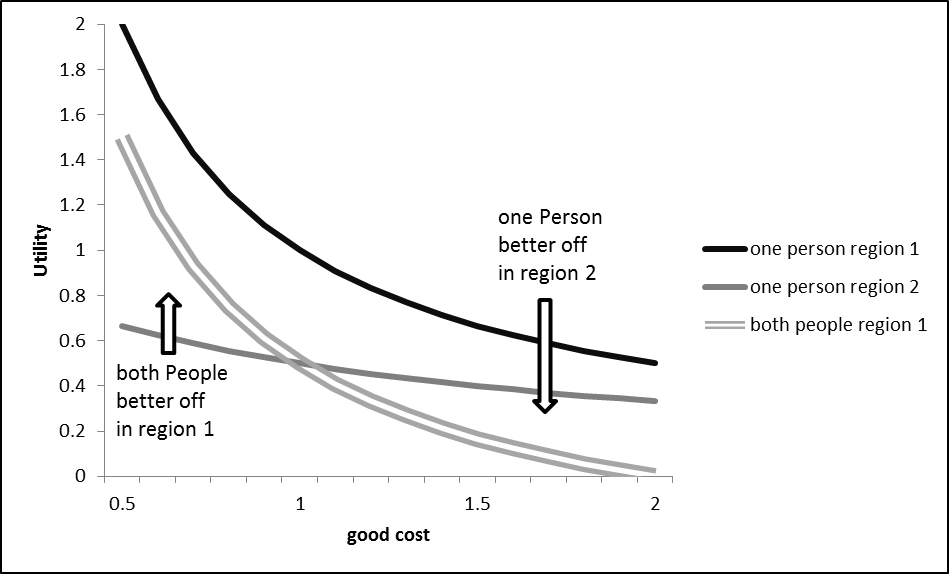
\includegraphics[width=0.9\textwidth]{ChapterTestingModels/Figures/2regionDiscreteGoodCostB&W}}
\caption{Two People, two regions. Wages & good cost $=1$. Density cost if two People in same region: 0.5, subtracted from wage. No distance cost in region 1, distance cost = $1$ in region 2.\label{fig:discretetworegioncomparison}}%
\end{figure}

What causes this opposite reaction? This section presents a small thought experiment based on the model framework using the simplest possible assumptions. There are two discrete regions and two People. Region one has no distance costs, but in region two it costs $1$ to deliver a unit of good. There is a single Firm in region one paying a wage of $1$. It produces $G$ at a base cost of $1$. As there is a distance charge in region two, it costs $2$ to buy one unit of good there. 

The two People must decide where to locate to maximise their utility. They can avoid distance costs by staying in region one, but if they both reside there, density costs are incurred. Let the density cost be zero if only one Person is present, and $0.5$ if both are in the same region. If so, subtract the density cost from the wage so it becomes $0.5$ for each. Utility is linear: $G = U$. 

Exclude the obviously poor choice of both residing in region two, where distance and density costs would be high: at least one Person would choose to minimise distance costs. This leaves only two possible states: both People in region one; or one Person in each region. Figure \ref{fig:discretetworegioncomparison} shows the utility for these two states, changing base good cost and distance cost (the spatial and non-spatial components of the total good cost).

It is better for one Person to move from region one to two where the single grey line is higher than the double. Increasing distance cost (sub-figure \ref{fig:discreteregiondelcost}) is agglomerating: while it is better for one person to move to region two when distance costs are below $1$, as they go beyond this, sharing region one with the other Person becomes utility-maximising. Conversely, increasing the base good cost (sub-figure \ref{fig:discreteregiongoodcost}) is centrifugal: as it increases past $1$, one Person will find moving away from the centre the best choice.

If a Person does move from a high-density spot, they leave another Person behind with higher utility than them: as soon as they decide to move to region two (single grey line), the other Person  gains a permanent utility advantage in region one (black line). The reverse is also true: if moving to region one is best, this will drag the utility of the existing resident down. These are both obvious externalities: moving from one to two increases both People's utility - but the Person staying put actually benefits more. Moving from two to one increases only the mover's utility; the other pays a price in increased density.

The presence of these externalities as a mechanism for equilibrium is in contrast to their role in neoclassical models. Skitovsky's characterisation of them as ``the villain of the piece'' (section \ref{sec:externalities}) contrasts with how they function in this \gls{abm} context, where market interactions are nothing \emph{but} externalities. Each agents' buying decision in one moment change the prices others face in the next. The spatial outcome of the results presented here are externality-based in the same way.

%three person thought exp
\begin{figure}[p]
\centering
\subfloat[utility vs distance cost]
{\label{fig:discrete3del}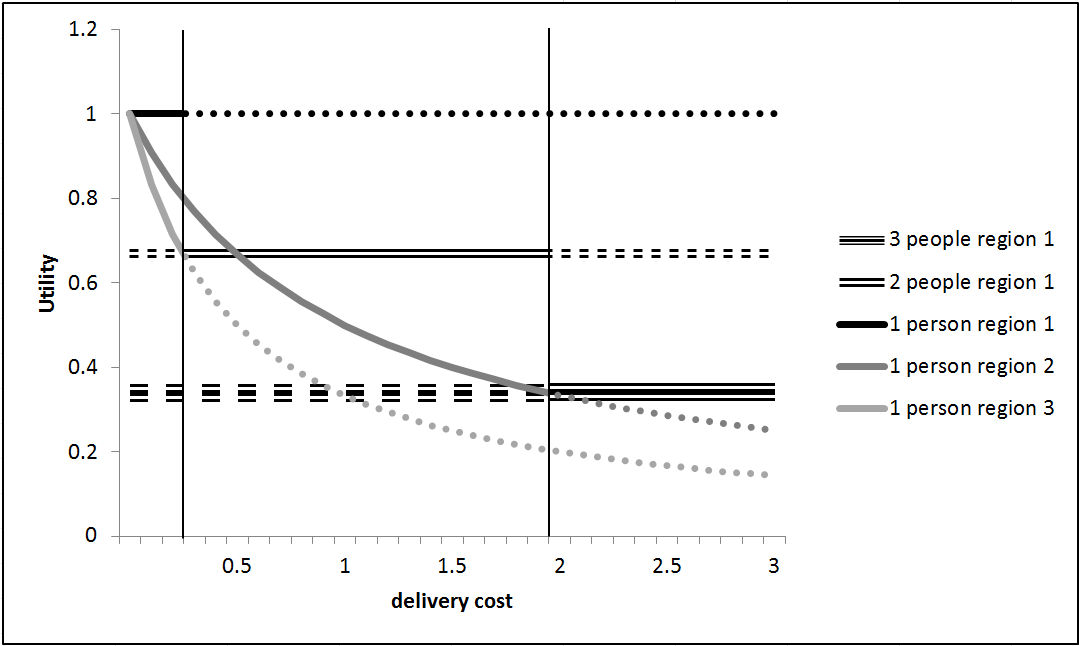
\includegraphics[width=0.9\textwidth]{ChapterTestingModels/Figures/3regionDelCost3finalfinal}}%
\hspace{0.2}  
\subfloat[utility vs base good cost]{\label{fig:discrete3good}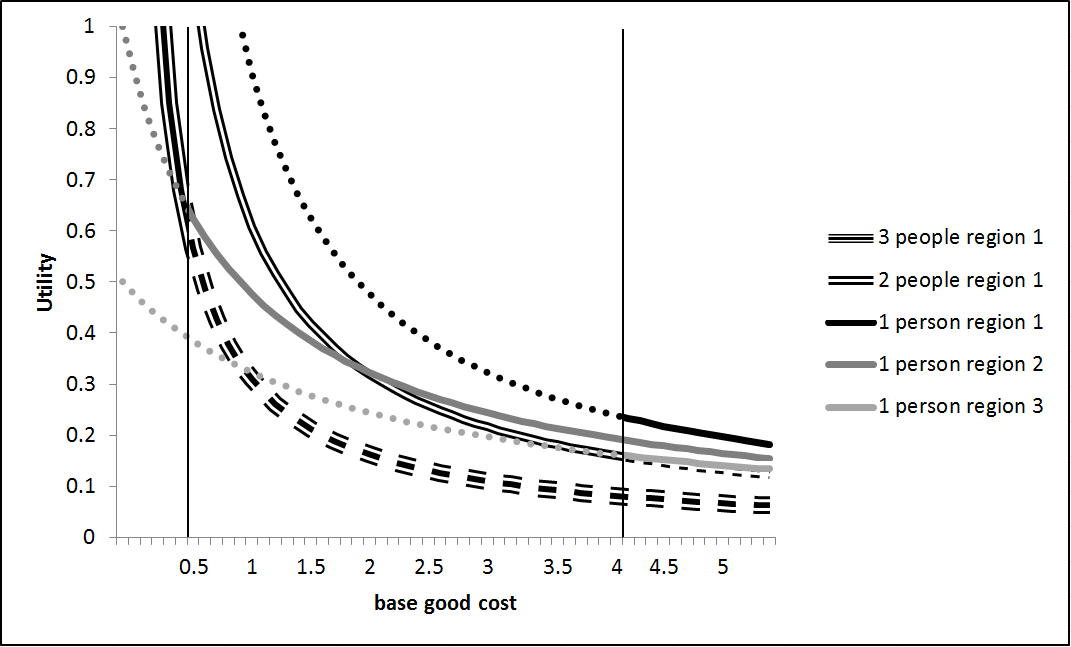
\includegraphics[width=0.9\textwidth]{ChapterTestingModels/Figures/3regionGoodCostFinal}}
\caption{Three People, three regions. Wages & good cost $=1$. Density cost if two People in same region: $1/3$; if three People are in the same region: $2/3$; subtracted from wage. No distance cost in region 1, distance cost = $1$ in region 2; = $2$ in region 3. Unbroken lines indicate optimal choices. \label{fig:discrete3regioncomparison}}%
\end{figure}

Extending the thought experiment to three People and three regions, with the third region a distance of $2$ from the first - twice as distant again as region 2 (figure \ref{fig:discrete3regioncomparison})  - produces more complex outcomes, but indicates where the pressure for spatial equilibrium comes from. Wage and good cost are again fixed to $1$. Density cost is $1/3$ if two People are present in one region and $2/3$ of all three People are present in one region.

It is made easier to understand be there being only three rational states for People to take: all three in region one; two in region one with another in region two; or one in each of the three regions. Looking at the case of changing distance cost and base good cost again (figures \ref{fig:discrete3del} and \ref{fig:discrete3good}) shows where the change between these three options takes place.

Each graph is split into three sections at two key cross-over points where People are incentivised to move. Unbroken lines indicate the utility-maximising choice in each case. Increasing distance costs is agglomerating: starting at lower values, People's best option is to spread out, one per region. Region three's resident has no incentive to move to region two: if two people reside there, its utility drops. They should stay put until `two people in region one' becomes the better option. That has a knock-on effect: the existing resident is made worse off. At the second cross-over, region two's new resident now finds region one better, increasing their utility but lowering that of the other two in the process.
%and region three's resident gets to move closer, becoming better-off in the process

For base good cost, the direction of agglomeration is different, but the outcome is the same: the pressure for spatial equilibrium comes from the external effect of one Person's optimal choice. Note, it is also possible to read off who will be incentivised to move. In the case of increasing base good cost, the utility of `2 in 1' - higher for cheaper goods - drops until a Person in region one finds moving right out to the edge the best option.

As noted in section \ref{sec:litbits}, the assumption of spatial equilibrium means that (as Glaeser put it) ``there must be no potential for arbitrage across space'' (\citealt{glaeser_cities_2008} p.4). The spatial equilibrium resulting from agent interaction in the models presented here do not allow agents to barter in the sense that `arbitrage' might imply, yet they are able to collectively produce near equilibrium spatial outcomes through a series of interactions, each causing an externality that pushes the model towards that equilibrium.


\subsection{Giving People a spread of costs \label{sec:vonThunen}}

\begin{figure}[p]
\centering
\subfloat[People in $R^2$ buying from central Firm]{\label{fig:vonWage}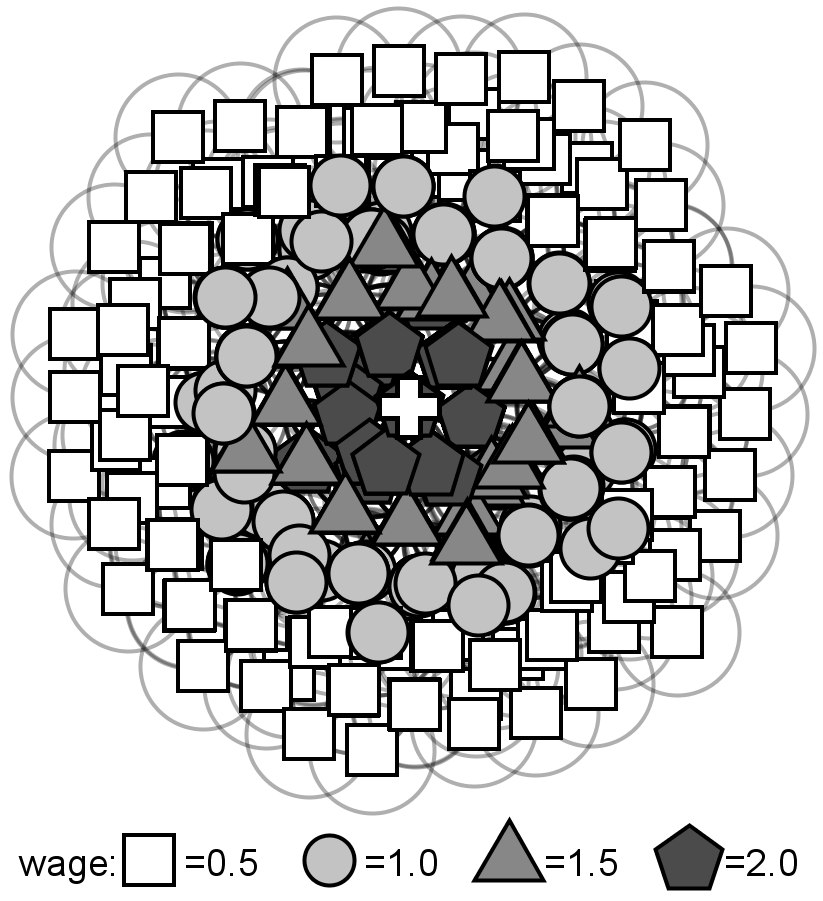
\includegraphics[width=0.6\textwidth]{ChapterTestingModels/Figures/JG_CEUS1_Wed-Dec-05-11_09_26-GMT-2012__MainViz}}%
\hspace{0.2}  
\subfloat[Utility versus distance to centre for each Person.]{\label{fig:vonWageUtility}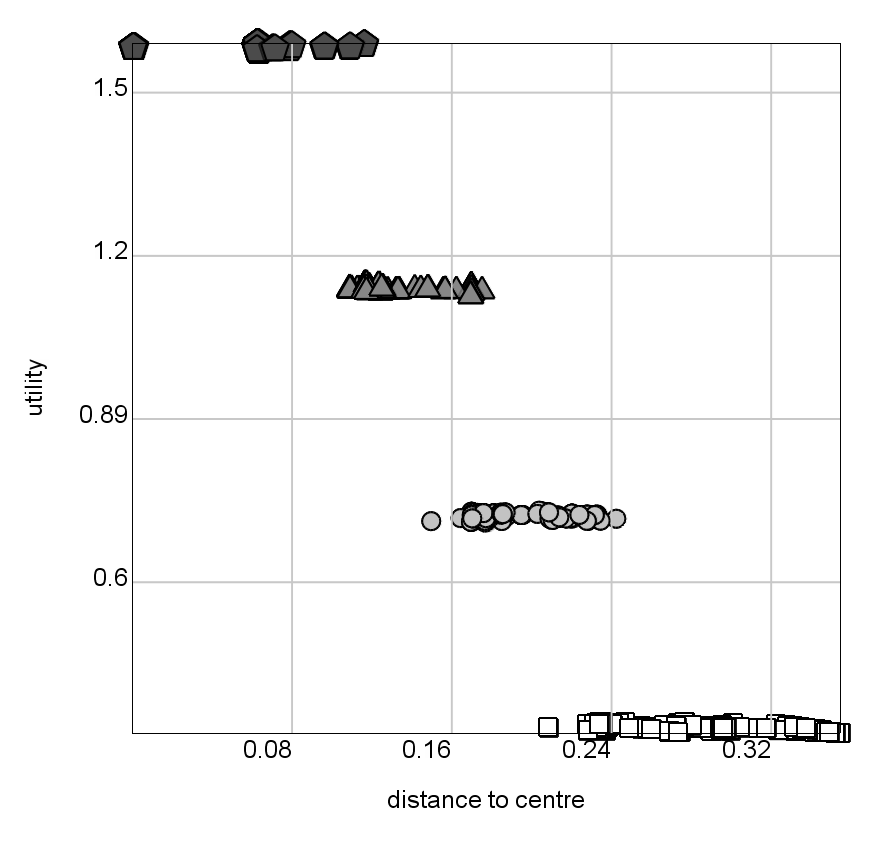
\includegraphics[width=0.7\textwidth]{ChapterTestingModels/Figures/JH_CEUS1_Wed-Dec-05-11_09_28-GMT-2012__distanceToCentralFirm_vs_maxUtility}}%
\caption{People set with variable wage, a quarter each set to values shown in the key. This key is used in the visualisation and correlation. Wealthier buy proximity. \label{fig:vonThunen}}%
\end{figure}

\begin{figure}[p]
\centering
\subfloat[People in $R^2$ buying from central Firm]{\label{fig:vonCommute}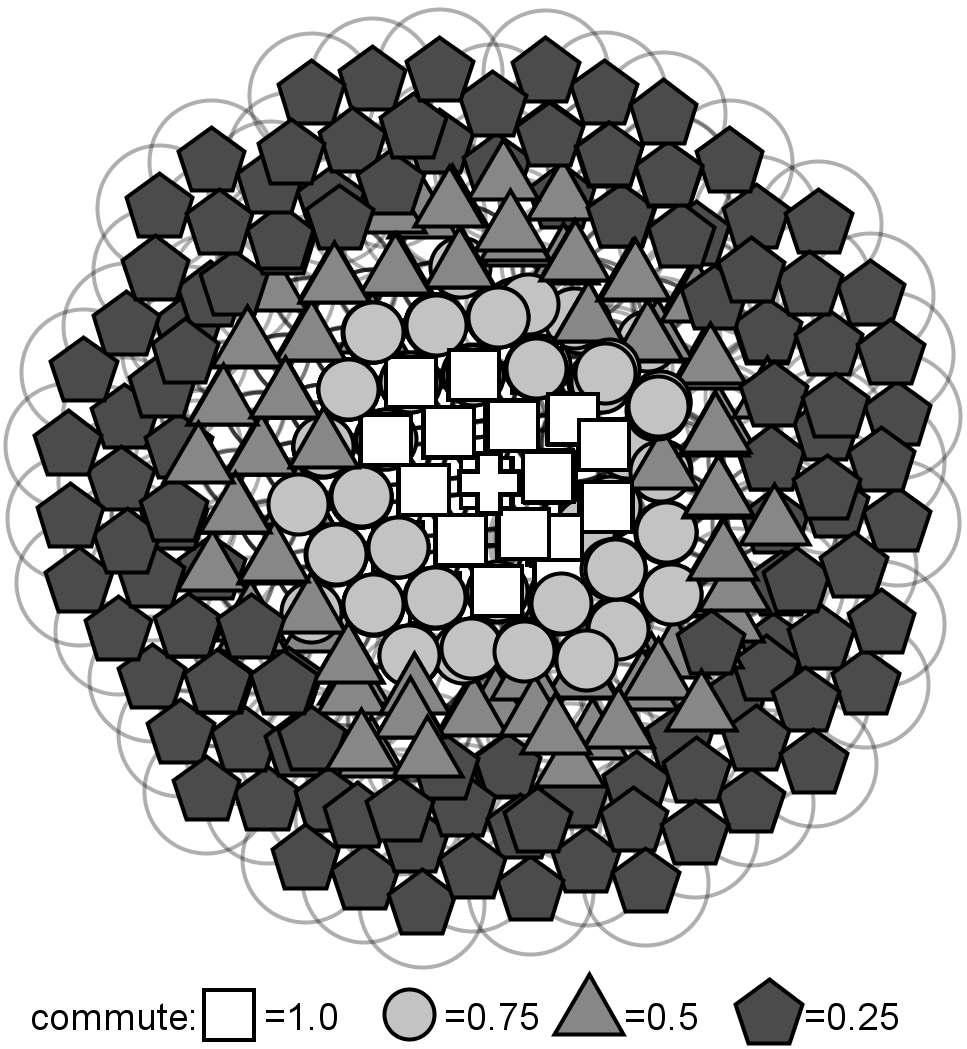
\includegraphics[width=0.6\textwidth]{ChapterTestingModels/Figures/JK_CEUS1_Wed-Dec-05-11_23_18-GMT-2012__MainViz}}%
\hspace{0.2}  
\subfloat[Utility versus distance to centre for each Person]{\label{fig:vonCommuteUtility}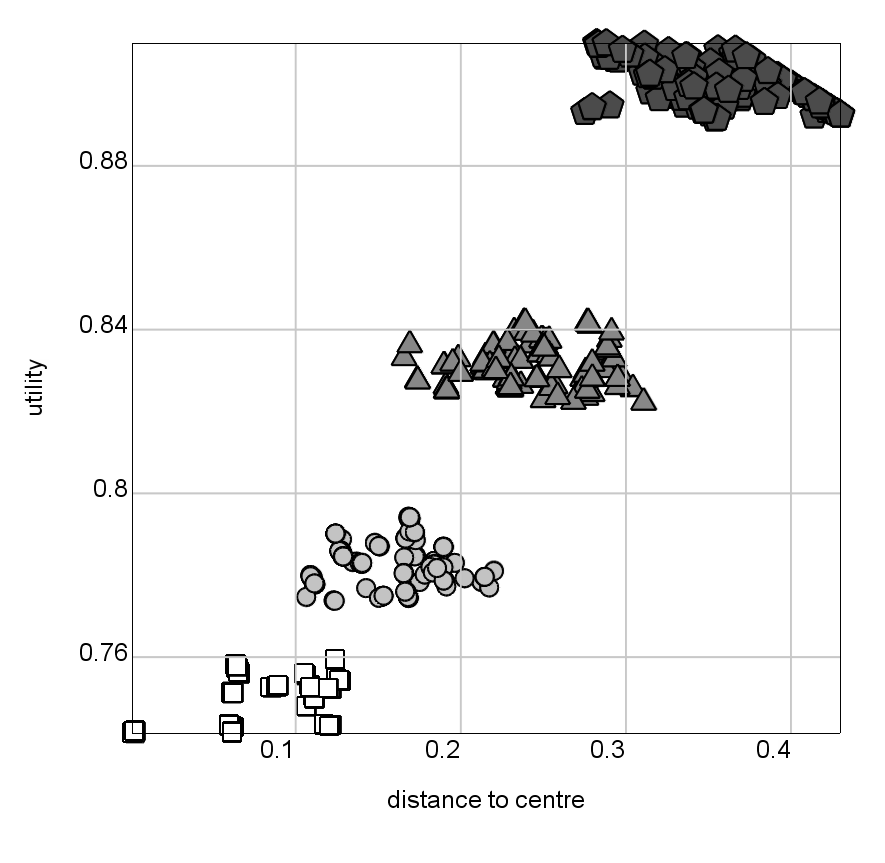
\includegraphics[width=0.7\textwidth]{ChapterTestingModels/Figures/JL_CEUS1_Wed-Dec-05-11_23_33-GMT-2012__distanceToCentralFirm_vs_maxUtility}}%
\caption{People set with variable commute cost, a quarter each set to values shown in the key. This key is used in the visualisation and correlation. Wealthier (paying less commute costs) buy distance.\label{fig:vonThunen2}}%
\end{figure}

This section presents a dramatic illustration of the opposite effect of spatial vs non spatial costs. This is a way to very clearly demonstrate the implications of spatial and non-spatial costs having the opposite effect as well as showing how von-Thunen like outcomes can emerge through agent interaction using the density cost approach. 

In figure \ref{fig:vonThunen}, four Firms are placed at the centre of the monocentric model. Each Firm has variable costs. Each Person is assigned permanently to a single Firm and cannot change. A quarter of People work for each of the four; the shaded shapes indicate which. Sub-figures \ref{fig:vonWage} and \ref{fig:vonWageUtility} show the spatial result if wages are varied between $0.5$ and $2$. Sub-figures \ref{fig:vonCommute} and \ref{fig:vonCommuteUtility} show the effect if commute cost is varied (from $0.25$ to $1$). Note that a higher commute cost is equivalent to a lower real wage. This variation is thus applied in reverse to make the diagrams comparable: in both cases, white squares have the lowest real wage and dark pentagons the highest. 

As dark-pentagon People are given a higher wage, unsurprisingly they also have the highest utility - but the place where they can find this depends on whether the cost is spatial or not. Being wealthier in a non-space cost allows a Person to buy a denser location and gain from proximity by reducing their commute cost. Having a cheaper commute allows more distance to be bought: the outskirts become the utility-maximising location.

Where the von Thunen approach uses a web of assumptions that include competition via landlords and assumed bidding curves, this example illustrates that a basic proximity cost and a parsimonious set of model assumptions, acting through agents' `second nature' decision-making externalised to the landscape, can produce a similarly clear emergent outcome. This is done with no market interaction. The discussion of whether this lack of a market is good or bad is taken up in the conclusion, in the context of the equilibrium outcomes of chapter \ref{chapter:connectedModels}. 
%In some ways, the result is more parsimonious than that other von thunen agent wotsit

\subsection{Love of Variety in a simple two-Firm scenario \label{sec:LoVresult}}

\begin{figure}[p]
\centering
\subfloat[]{\label{fig:LoVlow}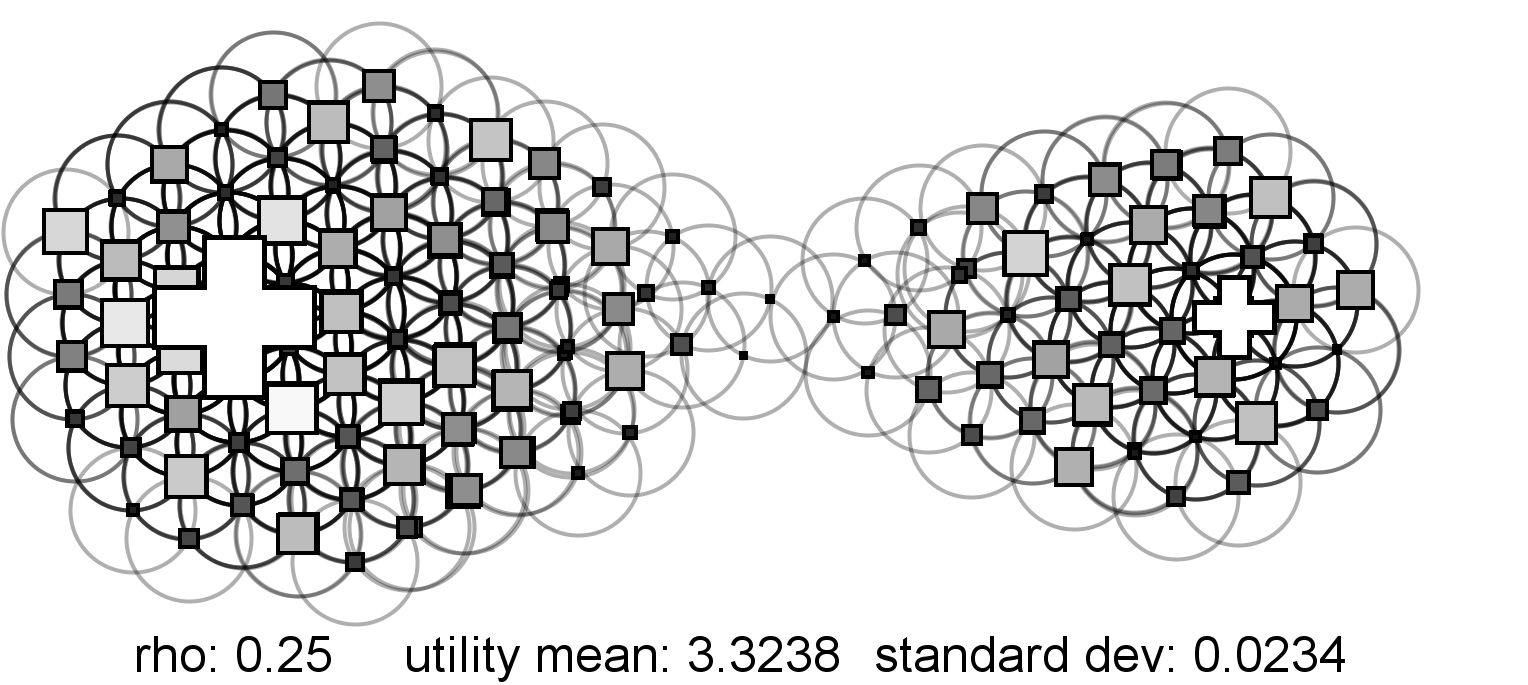
\includegraphics[height=45mm]{ChapterTestingModels/Figures/BothCESlowRho}}%
\hspace{0.2}  
\subfloat[]{\label{fig:LoVhigh}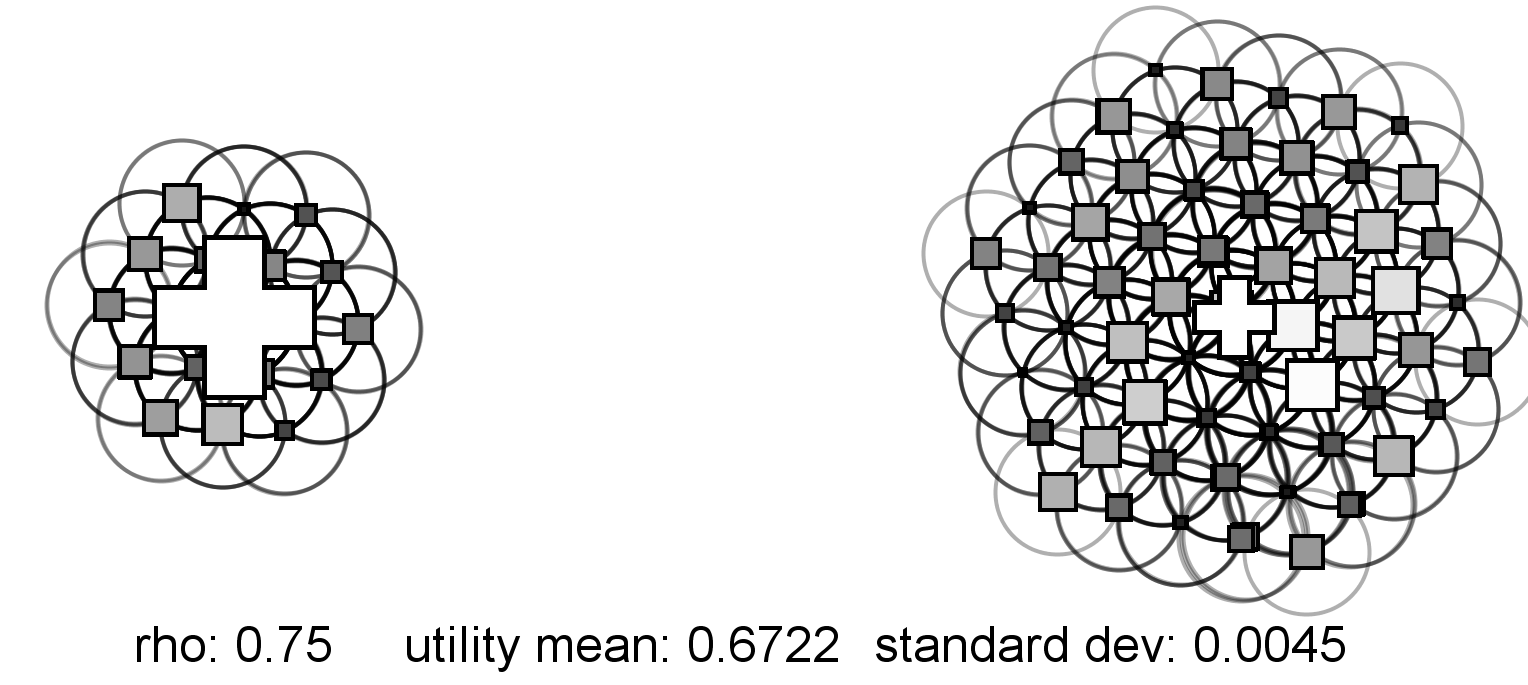
\includegraphics[height=45mm]{ChapterTestingModels/Figures/BothCEShighRho}}%
\hspace{0.2} 
\subfloat[]{\label{fig:LoVcorrelation}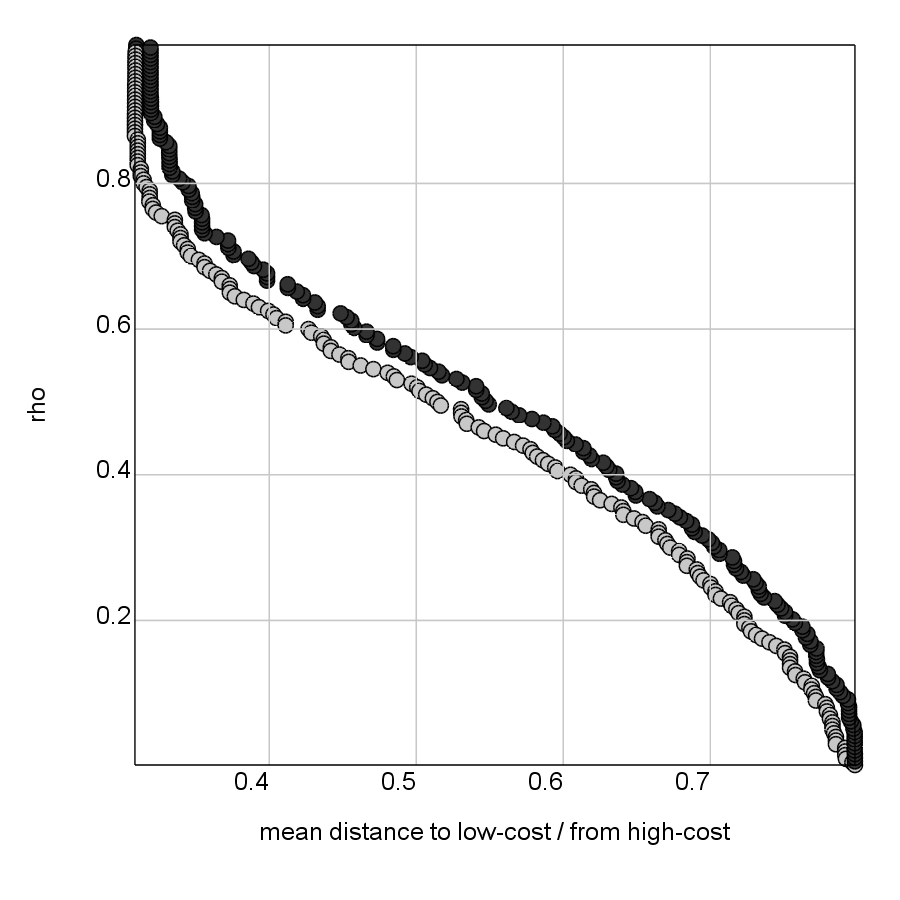
\includegraphics[width=0.68\textwidth]{ChapterTestingModels/Figures/JS_CEUS1_Wed-Dec-05-19_21_46-GMT-2012__distanceToCentralFirm_vs_rho}}%
\hspace{0.2}
\caption{Spatial effect of $\rho$: firm on right (small cross) has distance cost = $2$, the other = $4$.  $\rho$  is parameter-swept (positive in black, negative in grey) in increments of $0.005$. Single datapoint shown: average for all People, taken at spatial equilibrium. `Spatial equilibrium' is assumed when mean agent movement $<0.0001$ average over $10$ iterations. \label{fig:LoV}}%
\end{figure}

The \gls{ces} function has a very particular spatial effect in the presence of density costs. As section \ref{sec:utilspace} explained, if all goods have the same base price but vary in their distance, the closest will be the cheapest. So when $\rho = 1$ (and assuming demand can be met), only the closest good will be consumed. As $\rho \rightarrow 0$, however, more distant goods increasingly enter into a Person's optimal mix. In the example here, all other parameters are set and only `love of variety' is changed, to demonstrate what impact this can have upon spatial morphology in the presence of density costs. 

Two Firms are $1$ unit of distance apart. Distance costs for the two goods vary: one firm charges $2$ per unit distance, the other $4$ (the larger of the two crosses in figures \ref{fig:LoVlow} and \ref{fig:LoVhigh}). $500$ people are free to choose who they buy from and, in proportion to their `love of variety', they will buy a mix of the two available goods. There is no commute cost: they incur only the distance cost of the good and density cost.

In figure \ref{fig:LoVcorrelation}, the `love of variety' parameter ($\rho$) is swept from 0.99 to near zero, and back again to show any hysteresis. The same stability conditions used in section \ref{sec:spatialvsnon} are also applied. It is correlated against all People's mean distance from the low-cost Firm (so the inverse is their distance from the other Firm). The higher the `love of variety', the more People prefer to be near the more expensive of the two.

Figures for the mean and standard deviation of utility are provided in the visualisations. Utility is, unsurprisingly, higher for larger `love of variety' (as $\rho \rightarrow 0$) but there is very little difference across all People: it is close to a spatial equilibrium outcome. 

The role the presence of density costs is vital in this example. These set up a trade-off with proximity to Firms. Without a density cost, People could simply avoid distance costs by locating directly next to one of the two Firms (the `black hole' result). They would choose the Firm with the highest distance cost for all values of $\rho$. In the presence of density costs, however, two distinct `cores' emerge is $\rho$ is varied. For higher \gls{lov}, more People locate near to the higher distance-cost Firm. For lower \gls{lov}, when goods are more substitutable, more locate near to the low distance-cost Firm.

Why are more People choosing to locate closer to a higher distance cost source of goods when \gls{lov} is high (sub-figure \ref{fig:LoVlow})? Two things combine to cause the shift in morphology: density cost (imposing a distance cost) interacts with `love of variety' as it increases. In order to maximise the benefit of the mix of two goods, it becomes better to minimise delivery for the expensive good and buy the other from further away. If \gls{lov} drops and People gain less utility from a mix, they increasingly prefer locating near to the cheapest of the two. Though note, in sub-figure \ref{fig:LoVhigh}, some People are still centred around the more expensive Firm; this illustrates the trade-off that density cost causes.

There are points of indifference between the two `settlements' that develop around the two Firms, with density cost acting as the equilibriating force. This example illustrates that changing direct cost is not the sole determinant of morphology: changing utility alone can make the difference.

This model set-up is also the basis for the final result presented in section \ref{sec:tbmplusdensity}.

%The value of $\rho$ is also central to regional outcomes in Krugman's core model. However, the parameter does not solely represent utility, having also to act as a proxy for economies of scale and the determinant of firm number. One implication is that a change in people's tastes (due to an advertising campaign, say) can have a role to play in spatial outcomes.

\subsection{Spatial equilibria are not always utility equilibria \label{sec:notutilityeq}}

\begin{figure}[p]
\centering
\subfloat[$R^2$ space visualisation: density cost $=100$]{\label{fig:spatialEqViz1}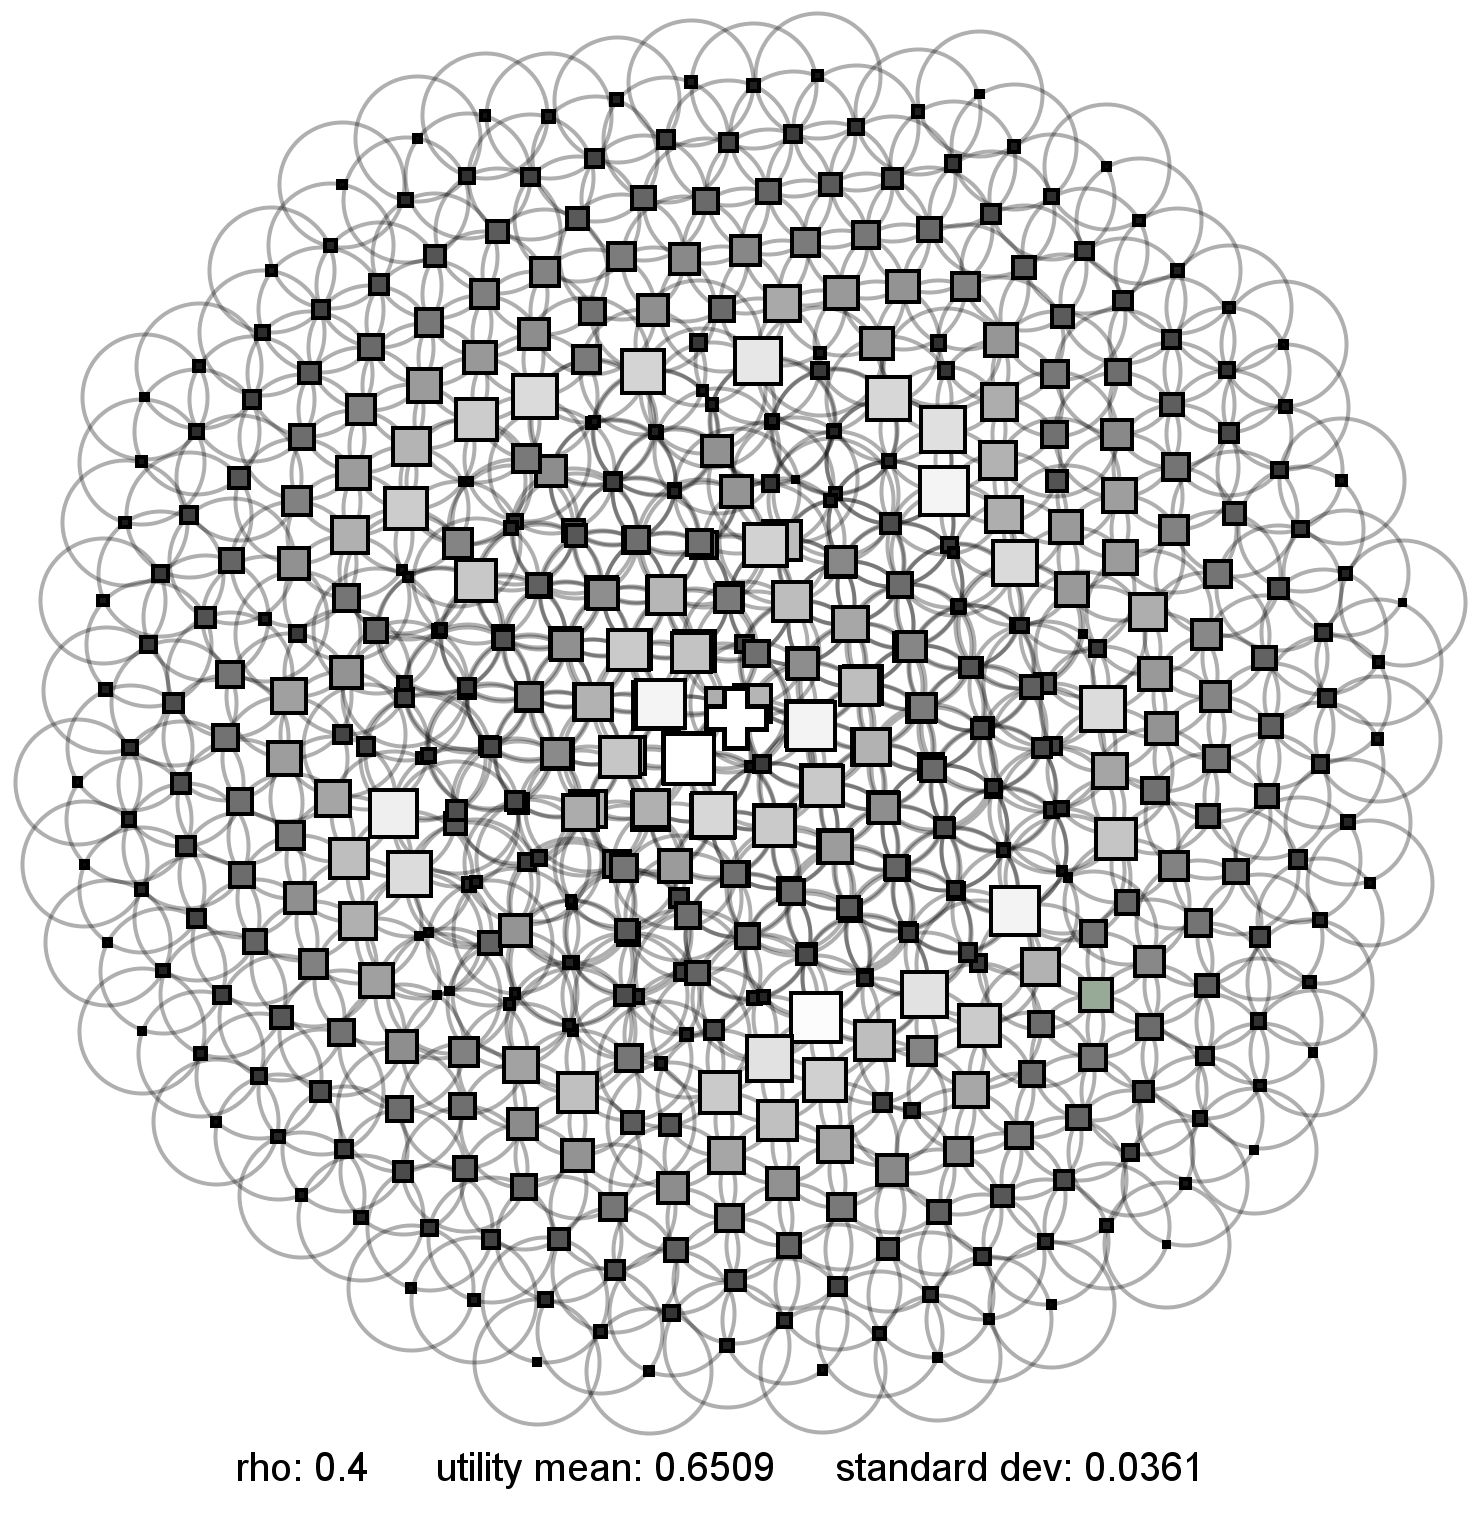
\includegraphics[width=0.65\textwidth]{ChapterTestingModels/Figures/RH_modelday_1399_CEUS1_Fri-Jun-07-16_23_49-BST-2013__MainVizedit}}%
\hspace{0.1}  
\subfloat[Utility versus distance to centre for each Person]{\label{fig:spatialEqGraph1}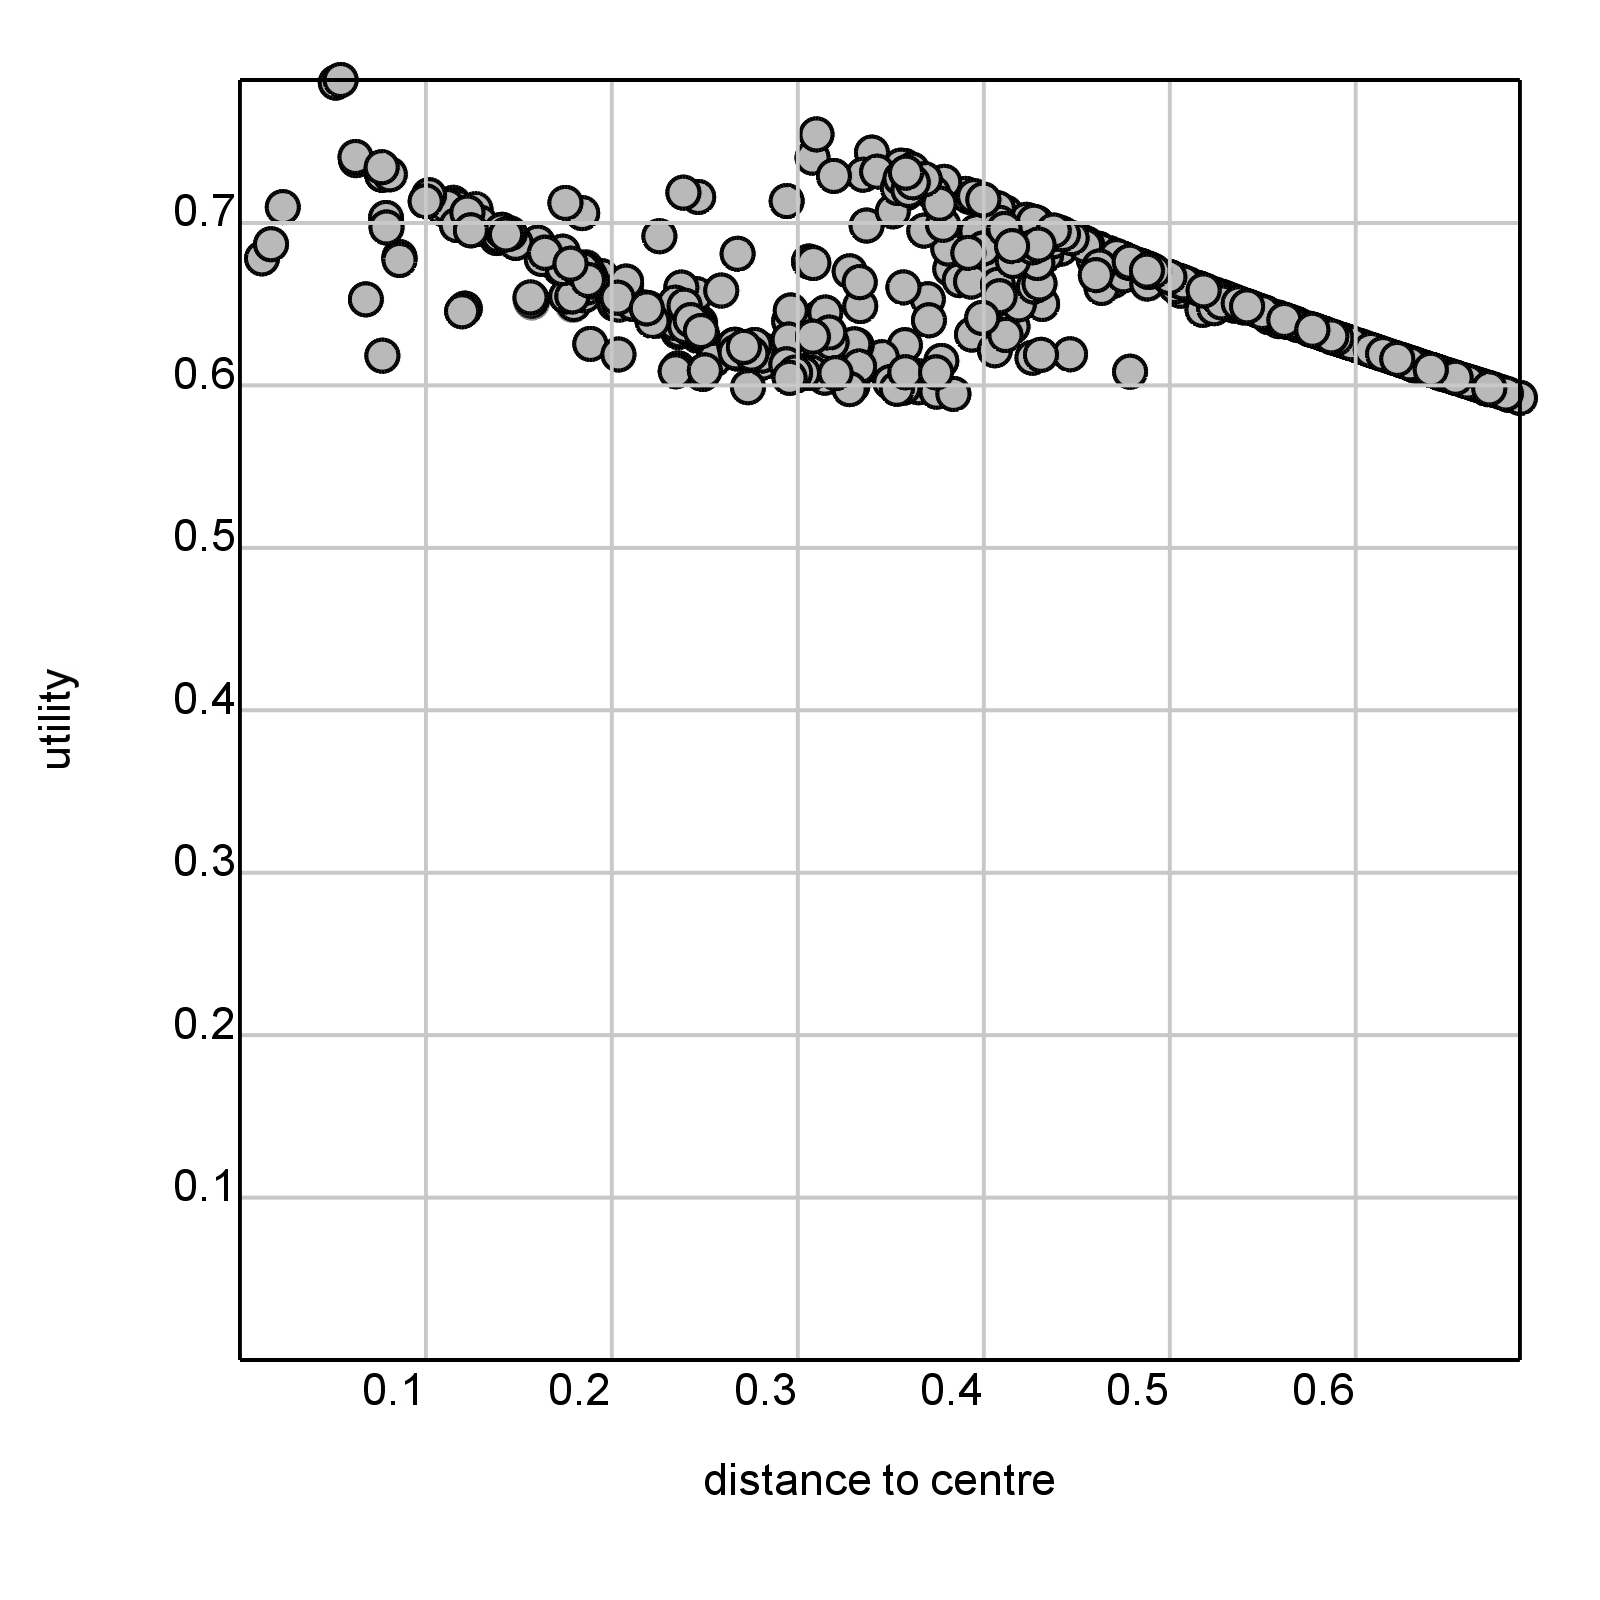
\includegraphics[width=0.7\textwidth]{ChapterTestingModels/Figures/RI_modelday_2197_CEUS1_Fri-Jun-07-16_24_42-BST-2013__distanceToCentralFirm_vs_maxUtility}}%
\caption{Density cost set to $100$: some People begin to prefer avoiding them altogether and locating on outskirts. People within settlement holding on to better locations before moving produces path-dependent morphology. Datapoint for each Person shown in graph. \label{fig:spatialEq1}}%
\end{figure}

\begin{figure}[p]
\centering
\subfloat[$R^2$ space visualisation: density cost $=500$]{\label{fig:spatialEqViz2}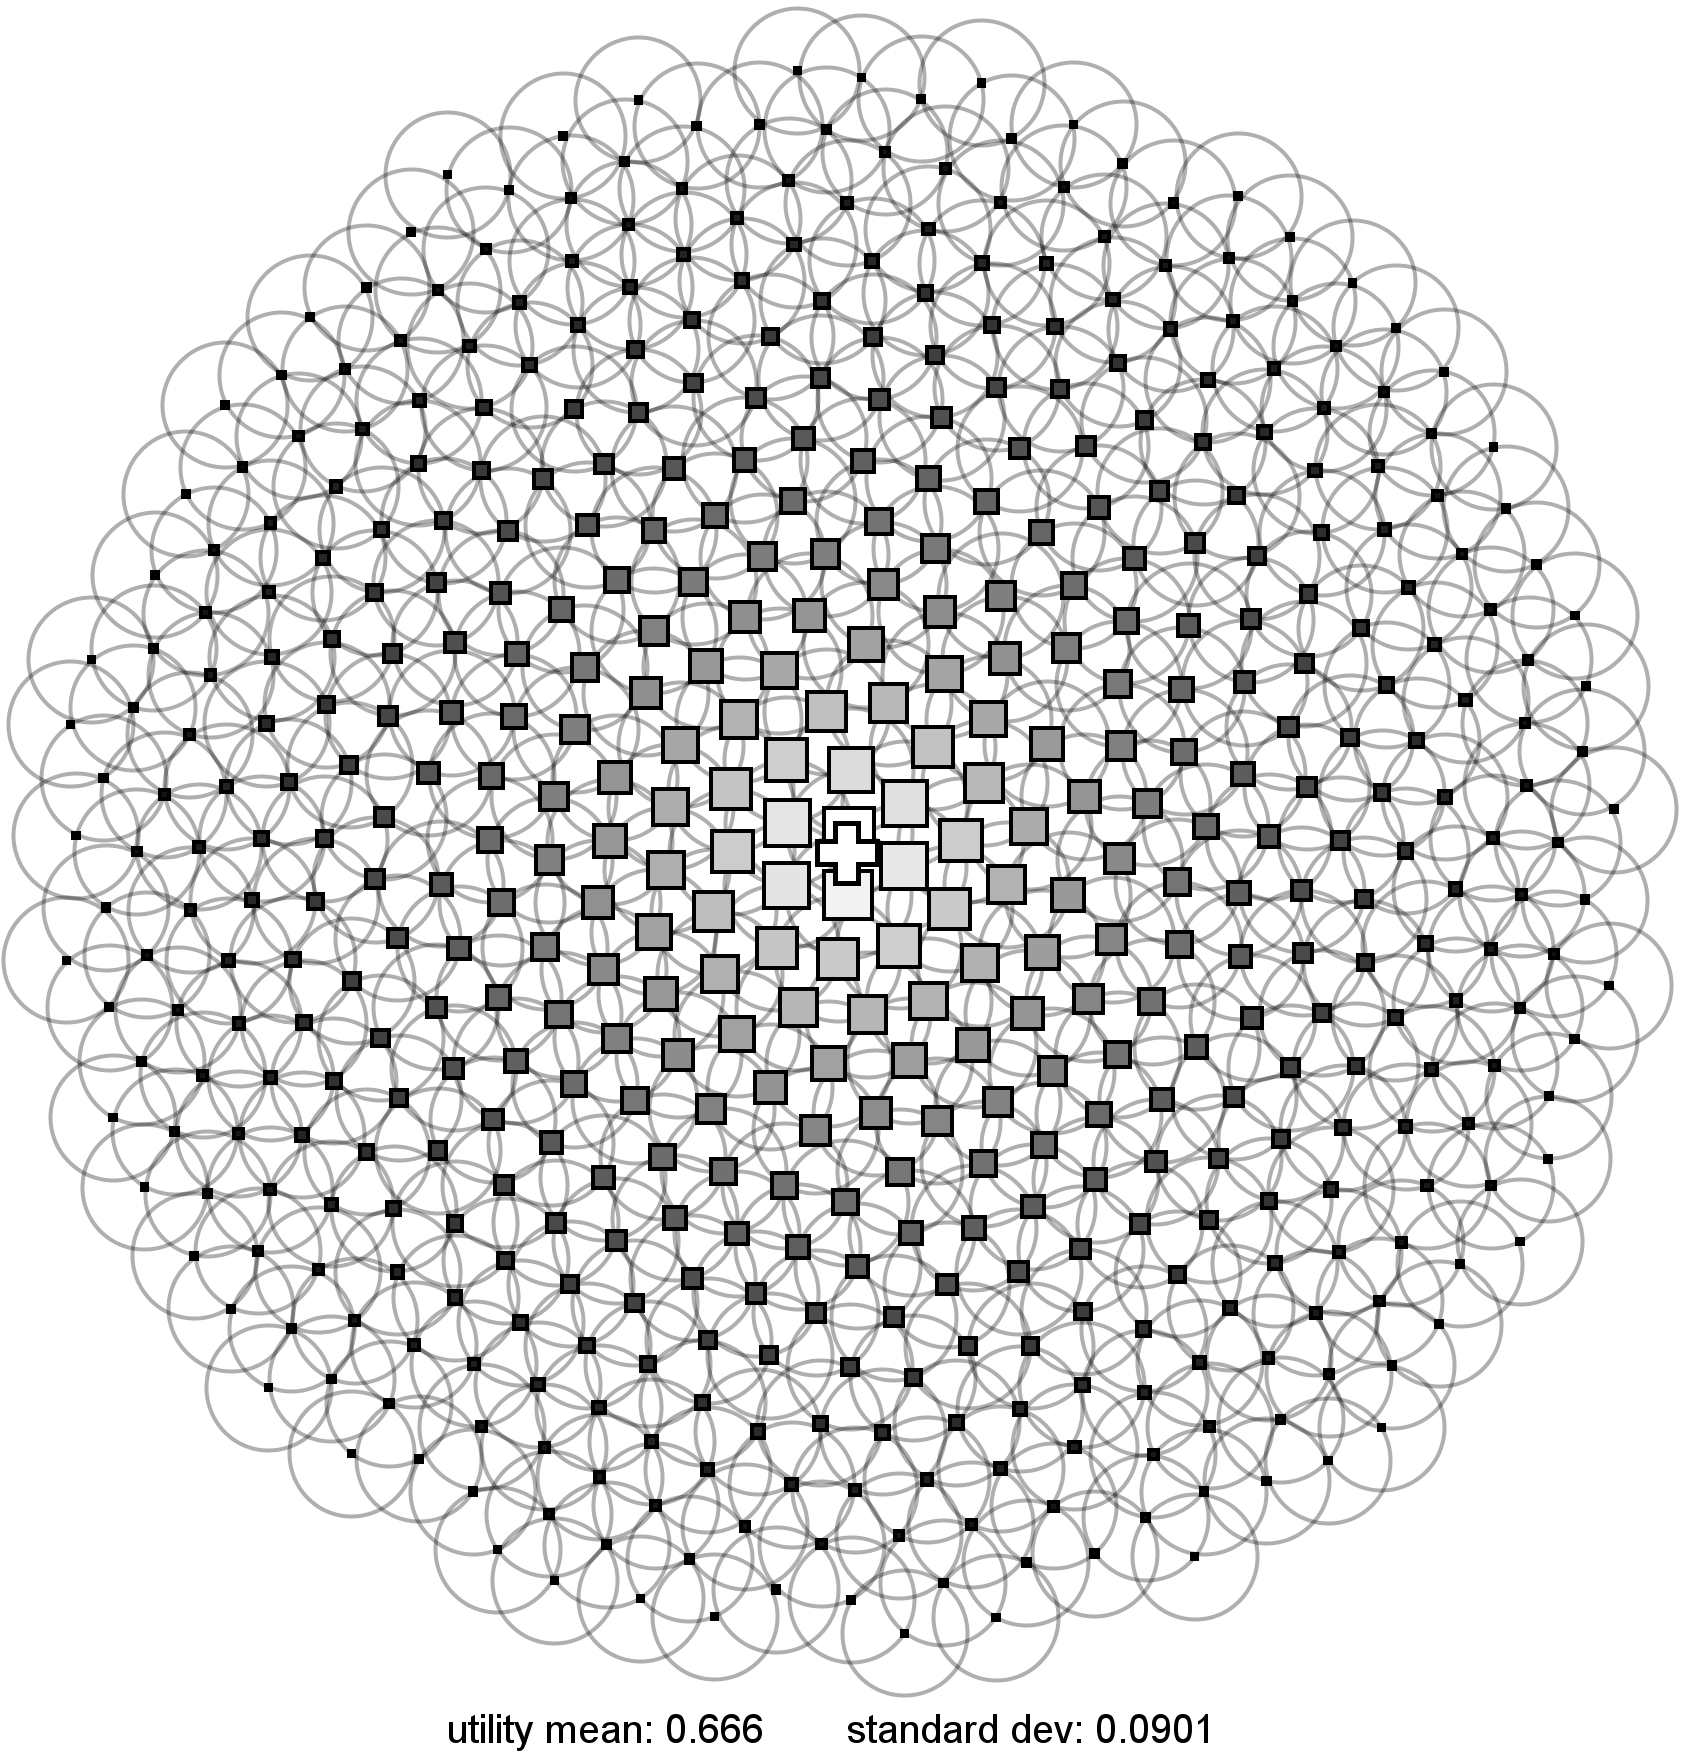
\includegraphics[width=0.65\textwidth]{ChapterTestingModels/Figures/RM_modelday_2008_CEUS1_Fri-Jun-07-17_29_44-BST-2013__MainVizEdit}}%
\hspace{0.1}  
\subfloat[Utility versus distance to centre for each Person]{\label{fig:spatialEqGraph2}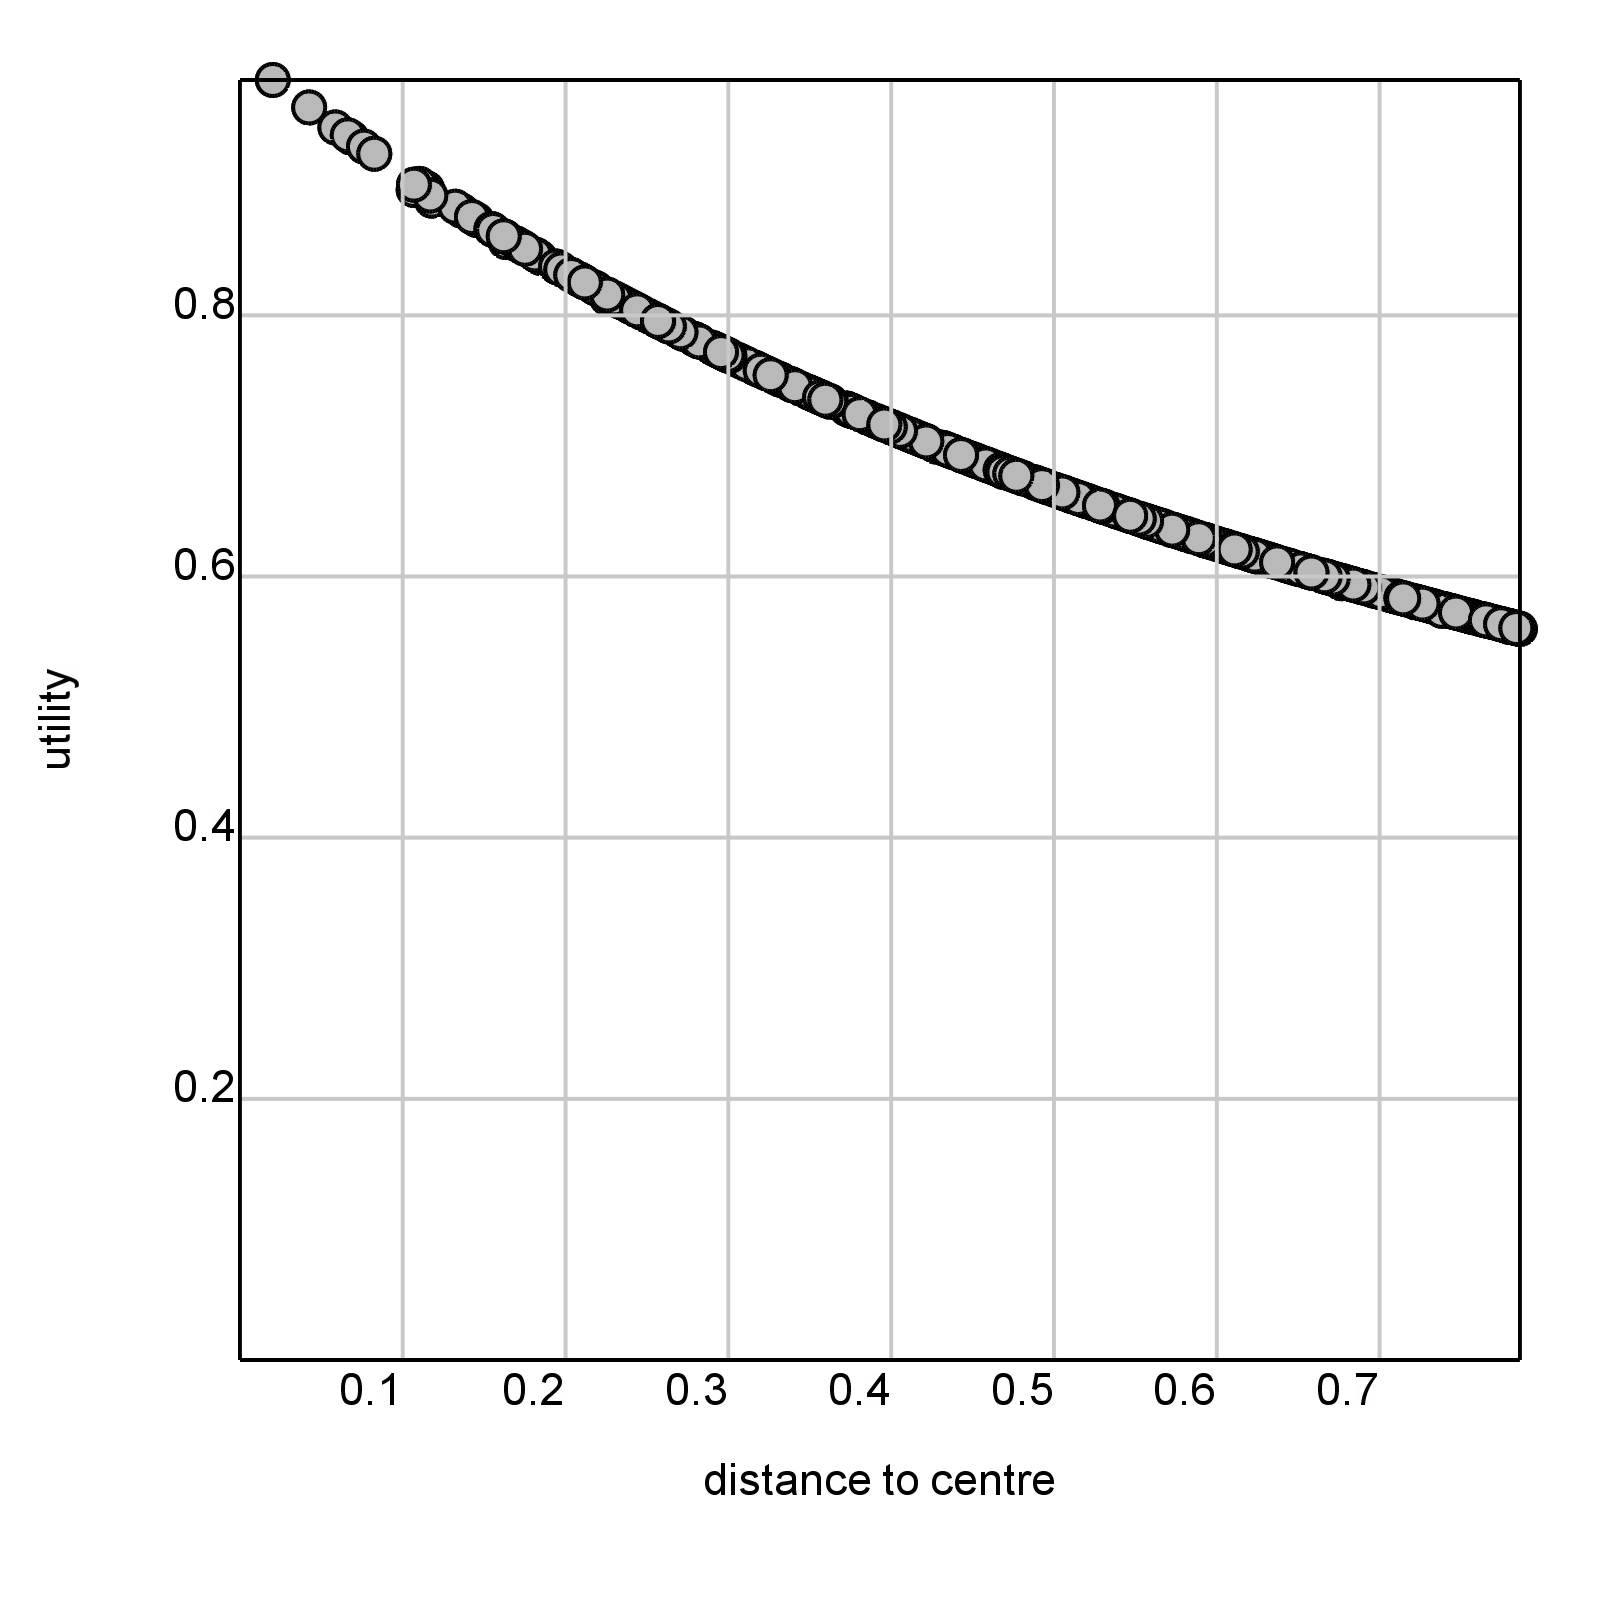
\includegraphics[width=0.7\textwidth]{ChapterTestingModels/Figures/RO_modelday_2458_CEUS1_Fri-Jun-07-17_30_12-BST-2013__distanceToCentralFirm_vs_maxUtility}}%
\caption{Density cost set to $500$: no Person finds incurring any density cost is better. Settlement fully spread; utility drops off for more distant agents. Datapoint for each Person shown in graph. \label{fig:spatialEq2}}%
\end{figure}

As mentioned above, there are a range of density cost values that allow People to make a trade off between density cost and distance. If they are able to do this, utility equilibriates: People self-organise into a spatial arrangement that allows them all to be equally well-off. However, this is not the case for all density cost values. 

The process begins on the outskirts of the settlement and works its way in to the centre as density costs are increased. Beginning at the outer edge, at a certain density cost, People find avoiding them altogether is their best choice: they locate on the edge where the available free space allows them to have a radius to themselves. At this level of density cost, spatial equilbrium begins to break down. If a Person, on their turn, finds moving right to the edge is best, the external effect is to lower density for others, thus relieving the pressure. The Person who moved first will be worse off than at least one Person they left behind.

Increasing density cost has two effects. Firstly, it is dispersive as it pushes People out towards the farthest edge. Secondly, the boundary of where density cost avoidance begins creeps in towards the centre as it goes up - until eventually every Person finds avoiding density cost is their best option. 

Figure \ref{fig:spatialEq1} illustrates this for a density cost of $100$; the boundary of complete density cost avoidance is not yet right at the centre. In sub-figure \ref{fig:spatialEqGraph2},  there is a characteristic dropping off of utility on the outskirts, indicated by the negatively sloped line of People's utility with those on the edge, with the furthest at a distance of approximately $0.7$ from the centre. The visualisation of the agents' $R&2$ spatial position in sub-figure \ref{fig:spatialEqViz1} shows the spatial patterning of utility, with many in the centre still incurring density cost. 

There is a clear second inner band in both figures where utility follows a negative slope. This is the result of two things. Firstly, the interaction of density cost with distance. Secondly, a path dependency in the model: gradually increasing the density cost reduces the utility of those who remain in place. They will only move if a higher-utility option presents itself. As sub-figure \ref{fig:spatialEqGraph2} indicates, there are distinct areas of the settlement with matching utility levels; People are indifferent between them. But if density cost increases, this will push those on the margin in the central area further out. 

Figure \ref{fig:spatialEq2} shows the result of all People avoiding density cost (at $500$) altogether. People's utility drops the further away they are from the centre (sub-figure \ref{fig:spatialEqGraph2}). At this extreme, spatial \emp{utility} equilibrium no longer exists. The remaining settlement is stable, however: no Person is able to find a better option. As the visualisation of their $R^2$ spatial organisation shows, those towards the centre have higher utility and have no incentive to give up their superior location. Those on the edge face the problem that moving further in will always incur the density cost. This is still a Nash equilibrium: no Person can take a unilateral decision that will make them better off. 

The implications of the above sections regarding mobile People are discussed in the concluding summary for this chapter (section \ref{sec:partialconcs}). Before that, the following section examines a scenario where People's location is fixed and two Firms attempt to optimise. 

\section{Mobile Firms \label{sec:mobFirms}}

In order to explore an example of Firms varying their location, the following two sections use a similar set-up. In both, all actors are on an $R^1$ line of length one. Two Firms can vary their location \textbf{only}: they have no control over price or wage, which are both set to one. Firms attempt to optimise their location using the method outlined in section \ref{sec:howFirmsAct}: they take an action and use a feedback between timesteps to judge if the action made them better or worse off, in terms of the amount of goods they sold. If successful, they will pursue the same action (in this case, continue in the same direction) until it stops making them better off. If they become worse off between time steps, they interpret this to mean `my action was a failure' and revert to their previous position.

First, section \ref{sec:hotellingesque} spreads fifty people evenly over the line, mimicking in discrete terms the spread of demand seen in Hotelling-style spatial models. Firms are able to optimise outcomes based on different settings for $\rho$ and distance costs, but their behaviour is somewhat erratic. Section \ref{sec:firmsLoV} explores the reasons for this in more depth, looking specifically at the problem of \gls{dmr} discussed in section \ref{sec:dmr}. 

This last section, by introduction coordination problems, is also sets the context for the final model chapter looking at the `transmission belt' model approach to making spatial agent coordination work.

\begin{comment}
The set-up for the models in this section is as follows:
\begin{itemize}
	\item An R^1 continuous line of distance $1$.
	\item Fifty People have fixed, evenly spaced locations along the line from $0$ to $1$. 
\item Two Firms are mobile, able to optimise their position to increase their revenue using the two-timestep feedback mechanism described in section \ref{sec:howFirmsAct}. 
\item People's wage and the base good cost are both set to $1$.
	\end{itemize}
\cmt{x-ref to `how firms act': make sure that section makes sense.}
\end{comment}
\subsection{Two Firms optimising location on a line \label{sec:hotellingesque}}

In this section, Firms attempt to optimise their position as just described. Demand from People is spread evenly over the line: if only a single Firm inhabited the model, it would want to locate exactly at the centre. The model asks: can Firms find optimal positions through their own feedback actions, given the presence of another Firm? 

The model diagrams in this section have the following set-up:

\begin{itemize}
	\item Values shown in the diagrams are means taken over the preceding ten thousand model iterations, in order to display the emergent outcomes rather than the more erratic `day-to-day' behaviour.
	\item The horizontal axis represents the distance of the $R^1$ line of length one. 
	\item The average amount (over the previous ten thousand time steps) of each Firm's good demanded by Each Person at their fixed location along the line is indicated above and below the central portion of the diagrams, and labelled for Firm $0$ and Firm $1$. The bars are shaded dark for lower values through to white for the highest. 
	\item Each Firm's mean position is shown by the point of the arrow, Firm $0$ pointing up and Firm $1$ pointing down into their respective demand graphs.
	\item The position arrows have bars indicating one standard deviation from the mean on either side.
	\item To give a better sense of the range of location options the Firms attempt, their actual locations over the last ten thousand time steps are indicated impressionistically below the mean position arrows. A single line is drawn per location choice using an `alpha' value so that more common choices build up and stand out in darker shades.
\end{itemize}

Note that, with no limitation on stock, each Person is able to have their full demand met (minus distance costs). So if both Firms are co-located (as in sub-figure \ref{fig:firmsLinesub1}) the Person nearest to each Firm, when they are both central, is able to acquire a mix of $0.5$ of each good. 

Figure \ref{fig:firmLines1} shows model outcomes for low distance costs (set to $1$). In sub-figure \ref{fig:firmsLinesub1}, \gls{lov} is high ($\rho=0.1$): the outcome is that Firms compete over a very small central spot, as indicated by a small standard deviation and a solid block of their actual location choices over the preceding ten thousand time steps. They are locked into a dynamic co-existence as their revenue-maximising spot is to provide a near-perfect mix of the two goods for all People. While sub-figure \ref{fig:firmsLinesub2} shows much the same average outcome when $\rho=1$ and goods are entirely subsitutable, the standard deviation and spread of location choices shows much more lively behaviour from the two Firms, spread out over the entire distance line. When $\rho$ is higher, competition for individual demand is much more binary: the cheaper Firm receives the payment. Nevertheless, the average outcome is still central.

\ref{fig:firmLines3} shows a single time-point snapshot to illustrate what demand does from moment to moment. In sub-figure \ref{fig:firmsLinesnap1}, where \gls{lov} is high, demand overlaps for the two Firms. In contrast, sub-figure \ref{fig:firmsLinesnap2} shows how demand is binary when goods are fully substitutable: People buy only the cheapest available to them, not a mix of the two. This cut-off does not show up in the averaged data in figure \ref{fig:firmLines2}.

In figure \ref{fig:firmLines2}, distance costs are raised to $20$. This increases the impact of distance on utilty, given the line consists only of distance $1$. Again, the sub-figures vary \gls{lov}. In sub-figure \ref{fig:firmsLinesub3}, when \gls{lov} is high, there is a tendency for the Firms towards the centre again but their location choices are considerably more spread out as they react to distance costs. In sub-figure \ref{fig:firmsLinesub4}, when goods are subtitutable, a Hotelling-like situation emerges: Firms (on average) find their revenue-maximising position at different ends of the line - though on average over ten thousand timesteps, there is an overlap in demand between them as they try new revenue-maximising locations. In the presence of higher distance costs, the Firms' spread of locations is actually higher when $\rho$ is lower, the reverse of the situation seen for lower distance costs. This is due to Firms more successfully `locking' into a spread of revenue-maximising locations in the high-substitutability scenario.

\begin{figure}[p]
\centering
\subfloat[High love of variety ($\rho=0.1$); distance cost $=1$]{\label{fig:firmsLinesub1}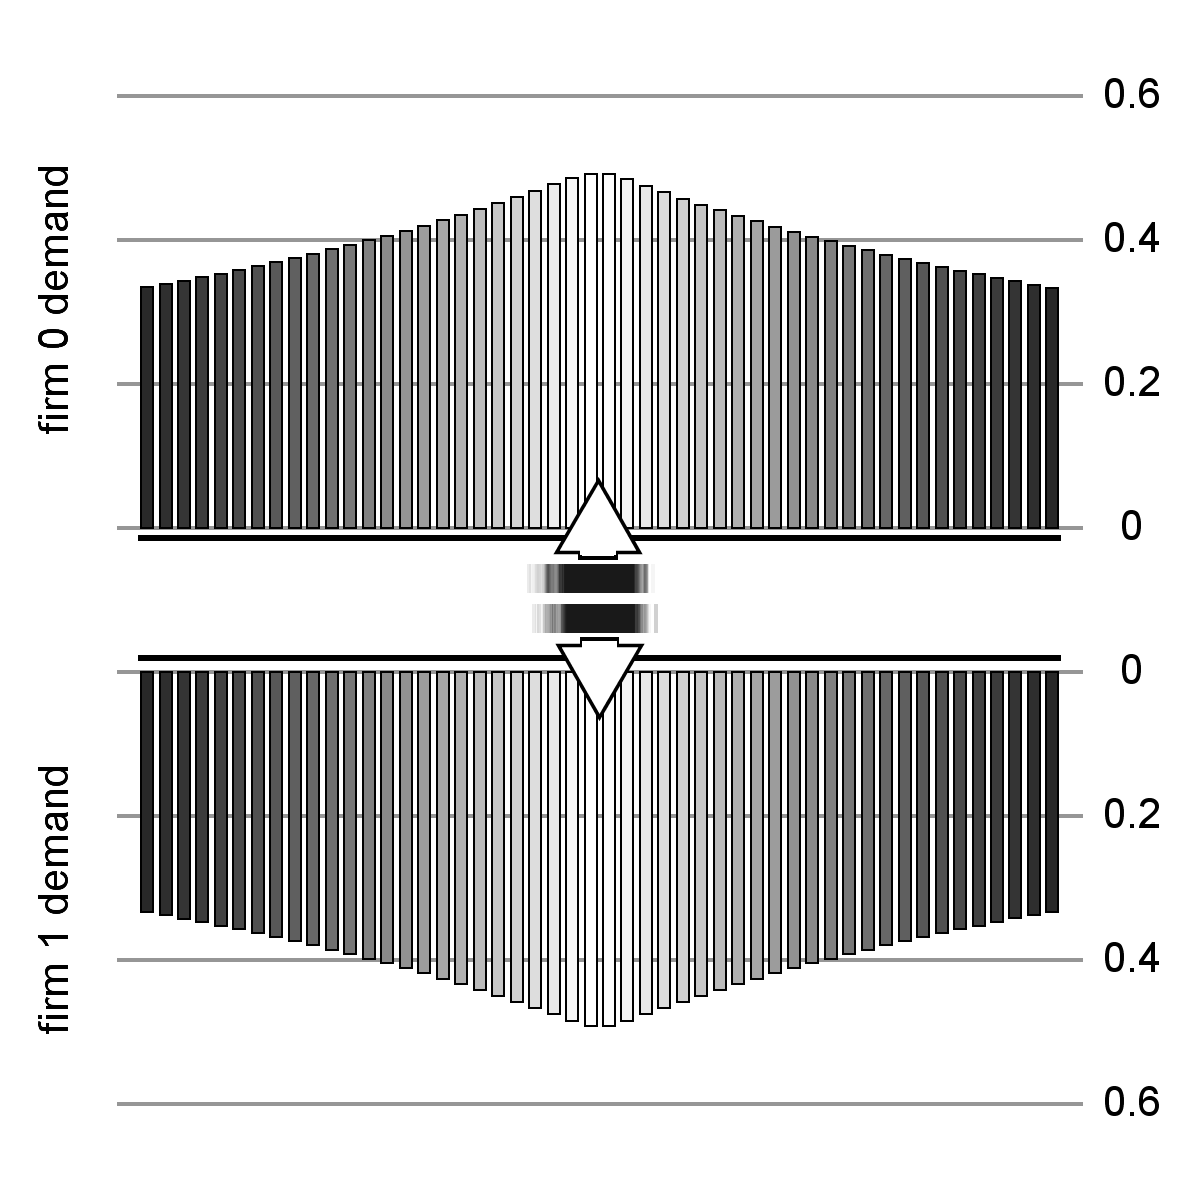
\includegraphics[width=0.67\columnwidth]{ChapterTestingModels/Figures/MO_modelday_52242_Hotelling_Line_DMR_Sat-May-25-12_33_01-BST-2013__MainVizrho0point1del1}}%
\hspace{0.1}  
\subfloat[High substitutability ($\rho=1$); distance cost $=1$]{\label{fig:firmsLinesub2}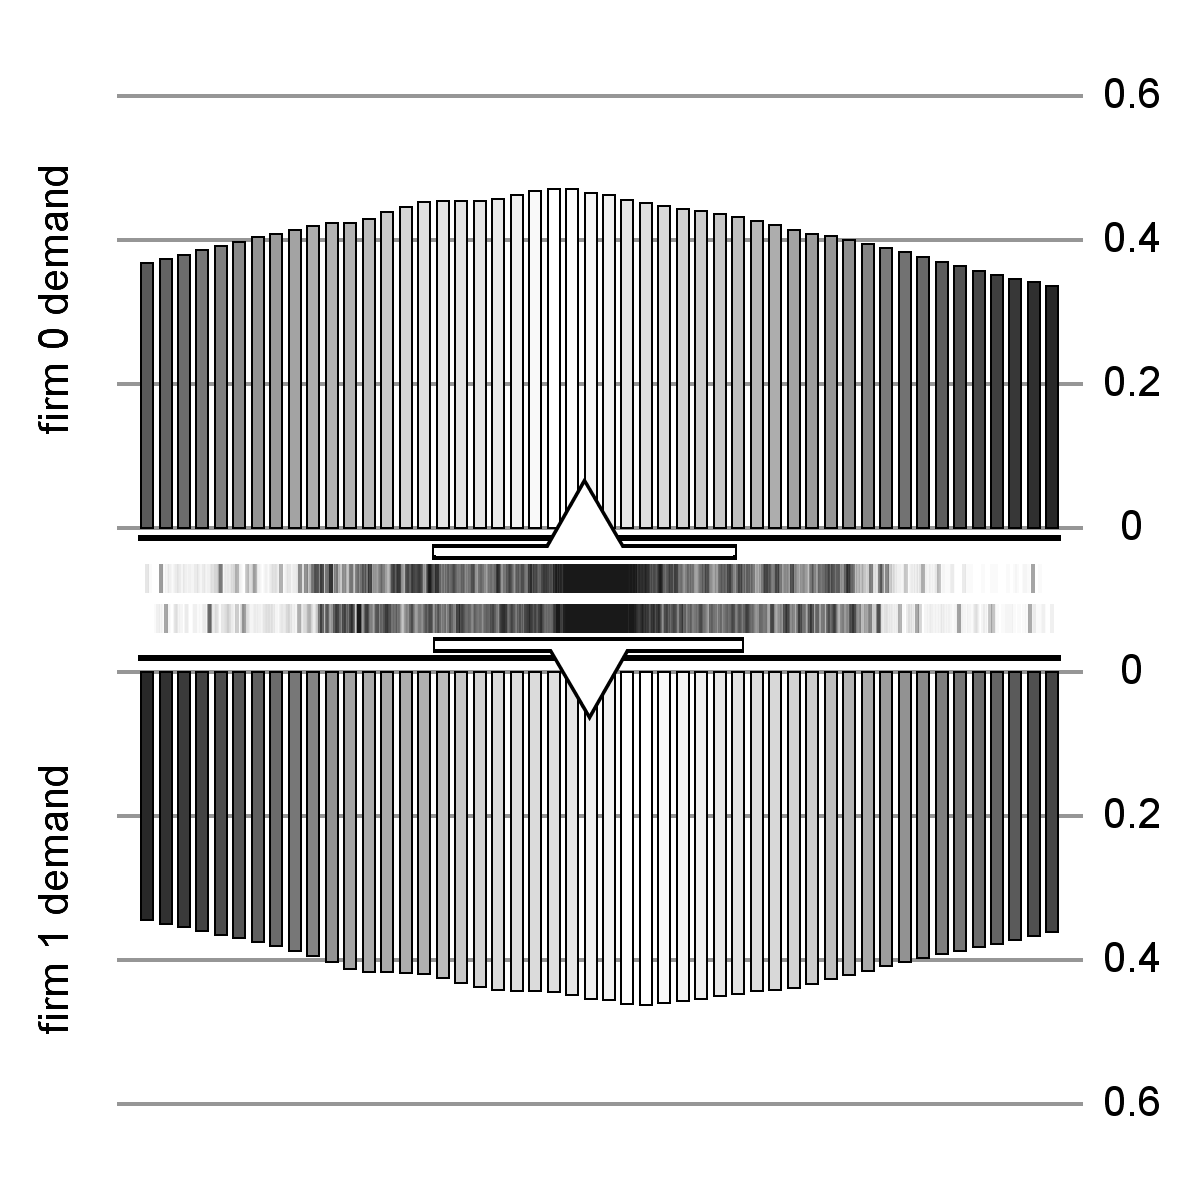
\includegraphics[width=0.67\textwidth]{ChapterTestingModels/Figures/MN_modelday_97098_Hotelling_Line_DMR_Sat-May-25-12_30_26-BST-2013__MainVizrho1del1}}
\caption{Two Firms optimise position on an $R^1$ line of length one. Fifty People spread evenly along the line from $0$ to $1$. $\rho$ varied, distance cost fixed at $1$. Means taken over $10000$ timesteps for Firm position and People's demand. White arrows shows Firms' mean location; white bars show one standard deviation each side of this; thin black vertical `barcode' lines between Firm arrows show actual positions taken by Firm over previous $10000$ timesteps. \label{fig:firmLines1}}%
\end{figure}

\begin{figure}[p]
\centering
\subfloat[High love of variety ($\rho=0.1$); distance cost $=20$]{\label{fig:firmsLinesub3}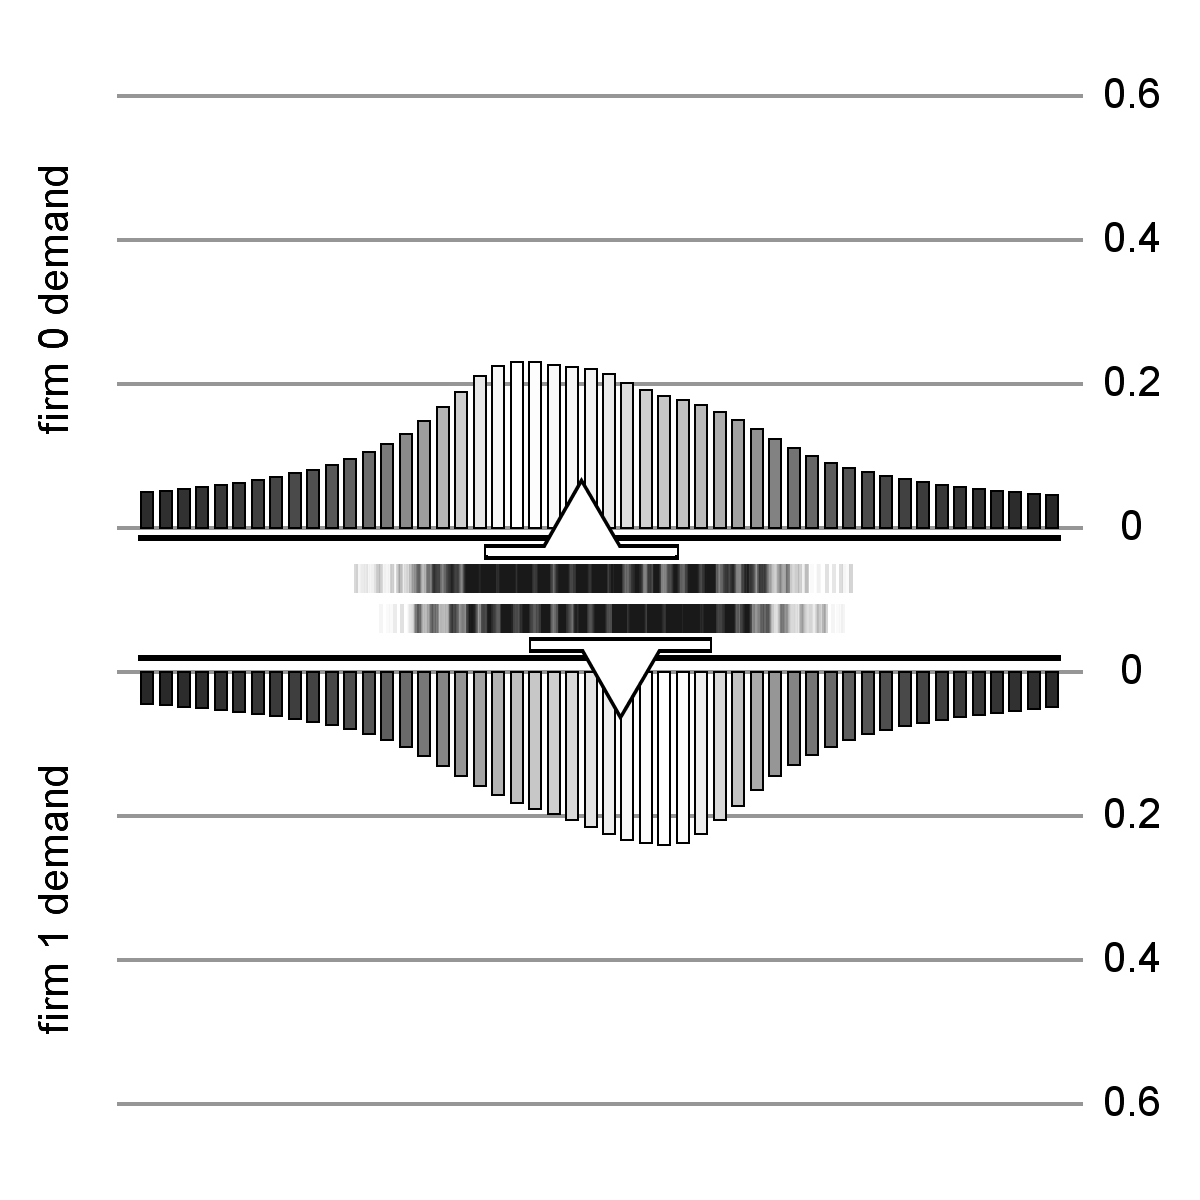
\includegraphics[width=0.67\columnwidth]{ChapterTestingModels/Figures/MP_modelday_88353_Hotelling_Line_DMR_Sat-May-25-12_38_12-BST-2013__MainVizrho0point1del20}}%
\hspace{0.1}  
\subfloat[High substitutability ($\rho=1$); distance cost $=20$]{\label{fig:firmsLinesub4}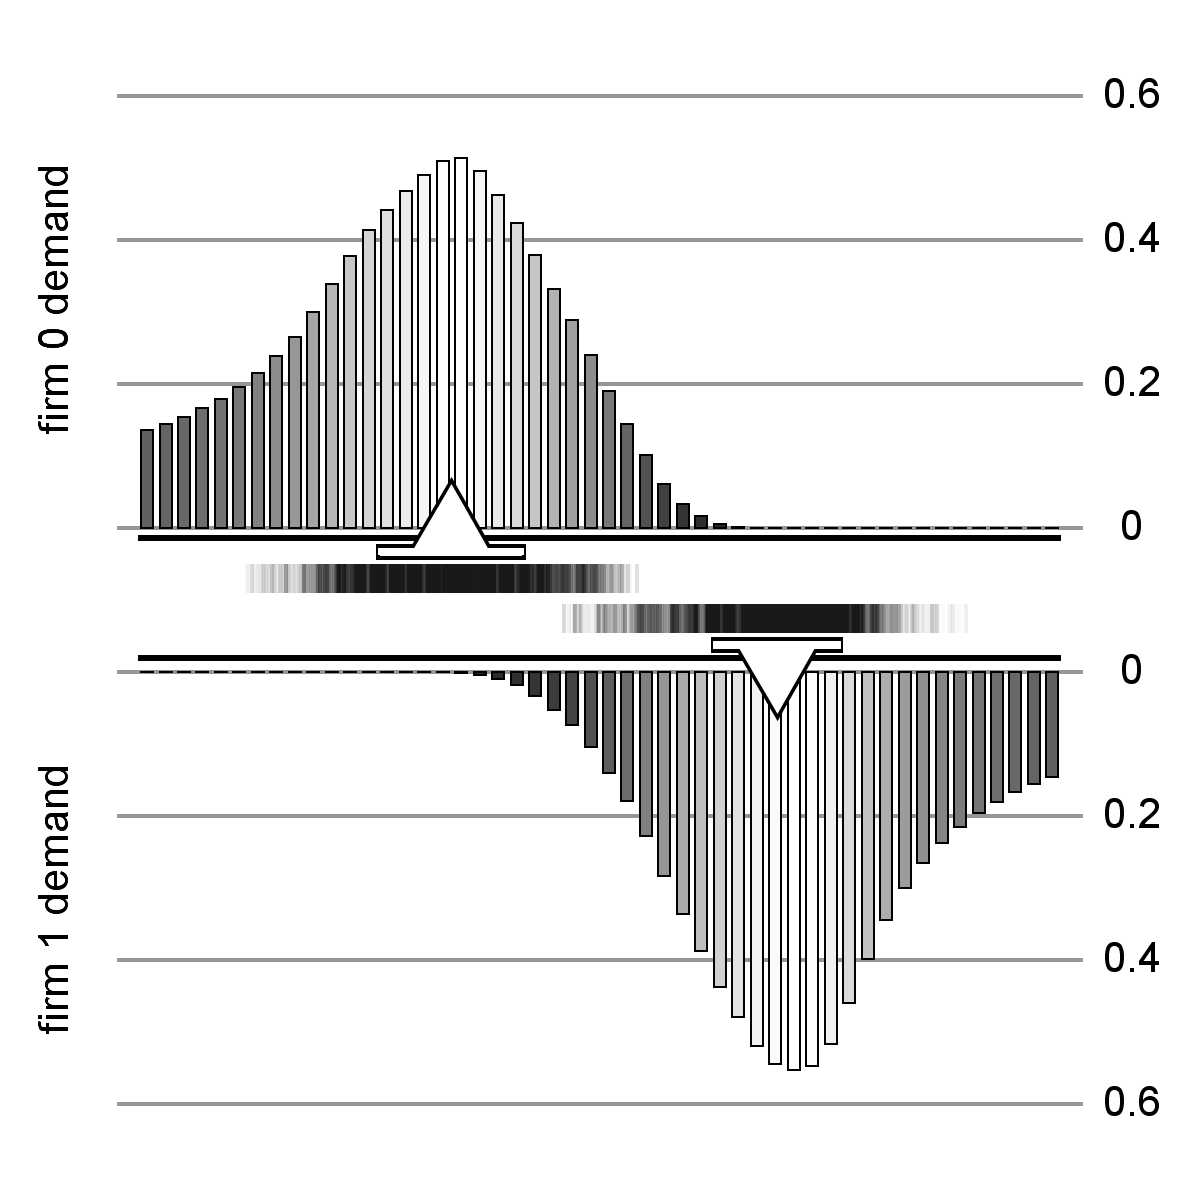
\includegraphics[width=0.67\textwidth]{ChapterTestingModels/Figures/MQ_modelday_98111_Hotelling_Line_DMR_Sat-May-25-12_40_58-BST-2013__MainVizrho1del20}}
\caption{Two Firms optimise position on an $R^1$ line of length one. Fifty People spread evenly along the line from $0$ to $1$. $\rho$ varied, distance cost fixed at $20$. Means taken over $10000$ timesteps for Firm position and People's demand. White arrows shows Firms' mean location; white bars show one standard deviation each side of this; thin black vertical `barcode' lines between Firm arrows show actual positions taken by Firm over previous $10000$ timesteps.  \label{fig:firmLines2}}%
\end{figure}

\begin{figure}[p]
\centering
\subfloat[High love of variety ($\rho=0.1$); distance cost $=20$]{\label{fig:firmsLinesnap1}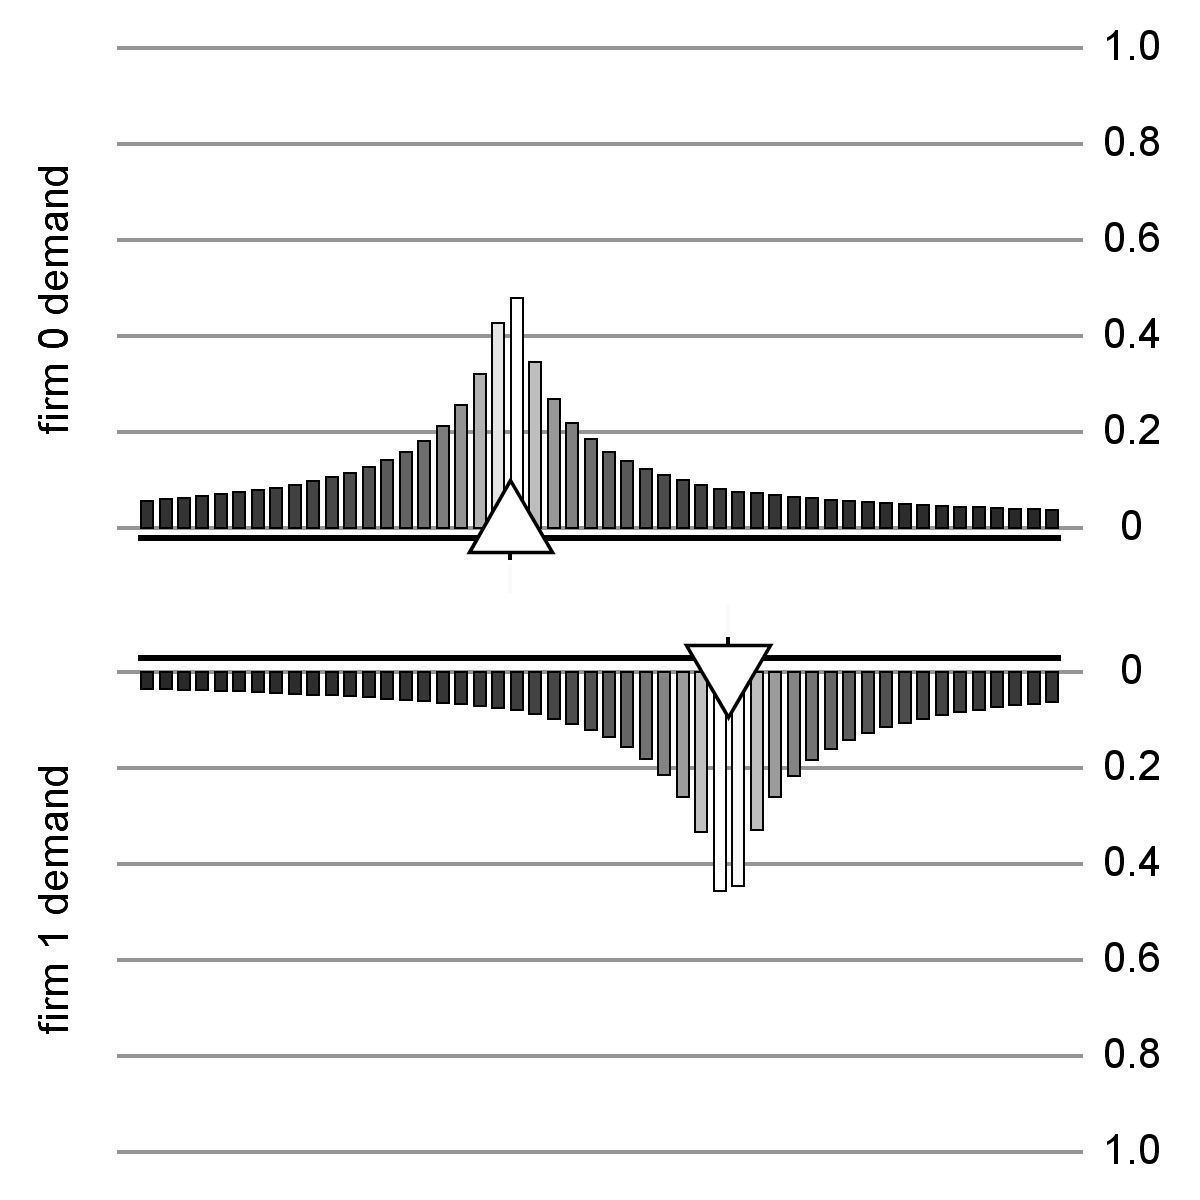
\includegraphics[width=0.7\columnwidth]{ChapterTestingModels/Figures/MV_modelday_906_Hotelling_Line_DMR_Sat-May-25-12_49_57-BST-2013__MainViz}}%
\hspace{0.1}  
\subfloat[High substitutability ($\rho=1$); distance cost $=20$]{\label{fig:firmsLinesnap2}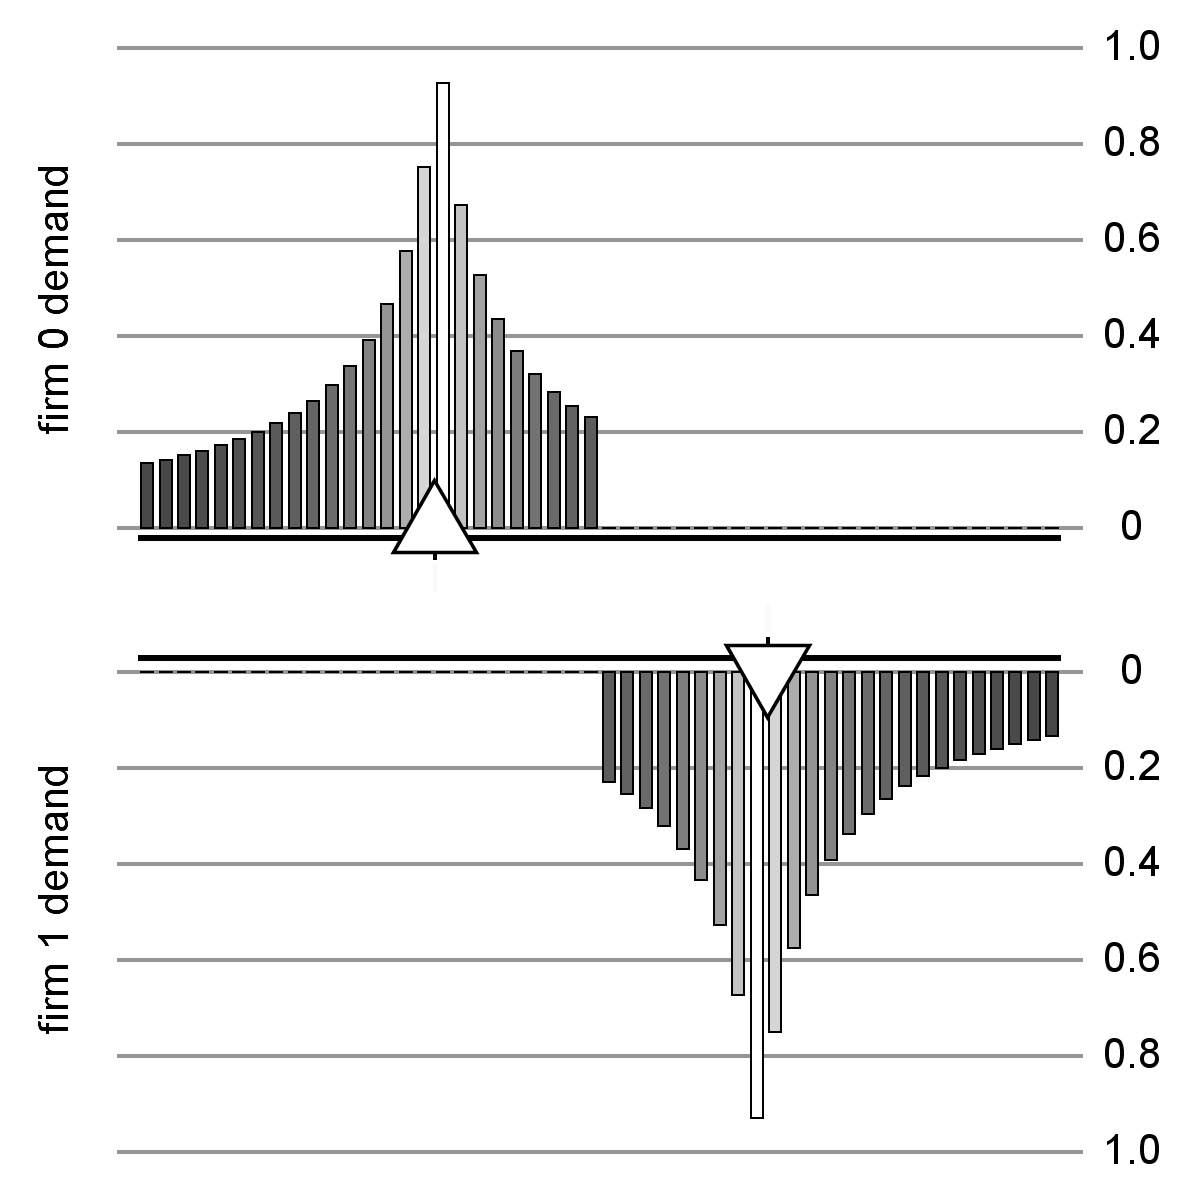
\includegraphics[width=0.7\textwidth]{ChapterTestingModels/Figures/MR_modelday_106_Hotelling_Line_DMR_Sat-May-25-12_49_16-BST-2013__MainViz}}
\caption{Single time-point snapshot: two Firms optimise position on an $R^1$ line of length one. Fifty People spread evenly along the line from $0$ to $1$. $\rho$ varied, distance cost fixed at $20$. \label{fig:firmLines3}}%
\end{figure}


Underlying these statistical outcomes, Firms ability to optimise their location using a location/revenue feedback mechanism appears quite weak. Why? The next section explores this problem in more depth. 

\subsection{`Data, meaning, response' with two Firms \label{sec:firmsLoV}}

The aim of this section is to investigate the interaction of Firms' signals to understand the \gls{dmr} problem (section \ref{sec:dmr}). It attempts to boil down the problem to the simplest possible elements to show that, even in a the most basic of examples, Firm agents attempting to optimise revenue through `sensed' market information alone can struggle to do so. It is an important example for understanding the limitations of Firm optimisation in the transmission belt model in chapter \ref{chapter:connectedModels}.

The model set-up is the same as in the previous section, apart from one key change: People are located only on a small subset of the $R^1$ line, between points $0.25$ and $0.75$. Each of the two Firms begins at opposite edges of the line. This model asks the Firms to play a `game'. A game terminates either when both Firms have succeeded in getting inside the range of space occupied by the People or ten thousand days has passed. 

The Firms can attempt to improve their revenue only by moving. Without competition from each other, their revenue-maximising position is near the centre of the People, where distance costs are minimised. Firms are making only this one decision: where to move? Getting closer to their market should, in theory, increase income - and indeed, if only a single Firm exists, it has no problem finding an income-maximising path. The rest of the world is static, so any change must be a consequence of its own actions. As soon as a second Firm is added, however, that is not the case. Confounding factors then mean they may fail to interpret the meaning of their cost signals correctly. 

In order to collect the data for figure \ref{fig:FirmGame1},  Firms play a large number of these games: utility noise levels are parameter-swept (see below) and for each value the random seed is altered a given number of times to then produce an average for all games with that value.

What is the rationale behind this? To put it into \gls{dmr} terms (see section \ref{sec:dmr}) a Firm has only one datum to act on, a change in revenue. The meaning of an increase is taken to be, `my previous action was successful'. Conversely, a drop in revenue is taken to mean that the action was counter-productive. This leads to the subsequent response: either repeat the action or reverse it. The broader meaning for the Firm in this situation is: `my actions can determine my revenue levels'. Problems arise when this meaning is incorrect: a Firm may take an action, but if its revenue levels are not determined solely by that action, there is scope for misinterpretation, and thus a faulty response. 

The aim is to provide a `god's eye view' of the Firms' goal in as simple a cost-signal setting as possible. The optimum they are aiming for is clear. Firms aiming between a subset line of People is, from the modeller's point of view, an entirely objective and clearly defined goal. At the same time, it is opaque to the Firms, since their `view' is restricted to revenue data. Although this looks like a Firm location model, here it is being used to examine the more general problem of conflicting signals involved in \gls{dmr}-type problems. Its purpose is to think about how Firms make decisions given (possibly noisy) information. Even putting aside that firms obviously do not `grope' their way to more productive locations, they would in reality be able to make much more informed location decisions. The question for this section is: in as simple an example as possible, what gets in the way of a Firm making an appropriate response to correctly interpreted data?
%If they were not forced to use revenue alone to `feel' their way, they could obviously be programmed to head straight for the centre of the circle. This makes it an easier example to consider than attempting to set prices. This combination - a single action, trying to optimise a single value - makes it useful for thinking about the problem. If Firms attempted to optimise other values (price or wage, for example) it would be considerably more opaque.
%The problem here is more akin to having to make pricing decisions in a small monopolistic competition situation, where both other firms' and people's actions affect outcomes.

%A full description of the setup for the `game' test is as follows. As mentioned, People are spread across a stationary line between spatial locations $0.25$ and $0.75$. Two Firms must find an optimal location that maximises their revenue. All prices and wages are fixed, and Firms' stock is unlimited. Distance costs are `iceberg': People pay a distance cost, but it `melts away' and Firms receive just the unit value. This means that, from the point of view of People, cost per unit drops as Firms draw closer. They can then afford to buy more. This means that a Firm's revenue-maximising location (in the absence of any others) is directly in the centre of the line of people. 

%If in $R^1$, this will be in one of the two available directions. If $R^2$, it will be a random vector defined by an angle and magnitude (as the magnitude is increased if the guess was successful
%A Firm's decision process is this:
%\begin{itemize}
%	\item At time $t-1$: Try a new location near to my current one; see section \ref{sec:howFirmsAct}).
%	\item At $t$: did my revenue improve?
%	\begin{itemize}
%	\item Yes: repeat the previous action, increasing the distance slightly
%	\item No: revert to last good location
%\end{itemize}
%\end{itemize}

\begin{figure}[p]
\centering
\subfloat[$noise = 0$]{\label{fig:fg11}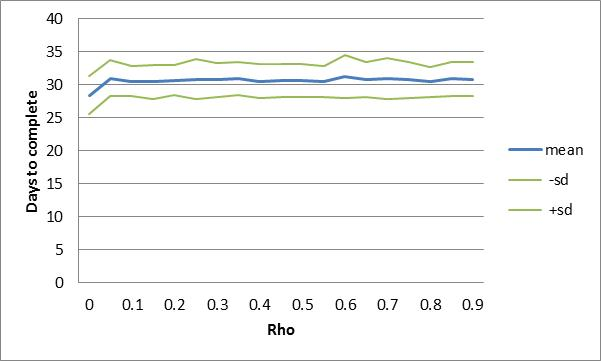
\includegraphics[width=0.7\columnwidth]{ChapterConnectedModels/Figures/FirmGame11}}%
\hspace{0.1}  
\subfloat[$noise = 0.1$]{\label{fig:fg12}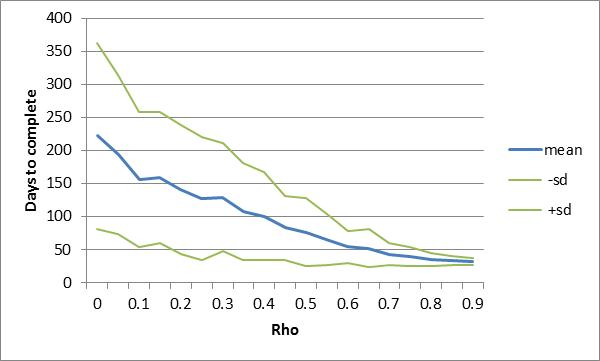
\includegraphics[width=0.7\textwidth]{ChapterConnectedModels/Figures/FirmGame12}}
\hspace{0.1}  
\subfloat[$noise = 0.5$]{\label{fig:fg13}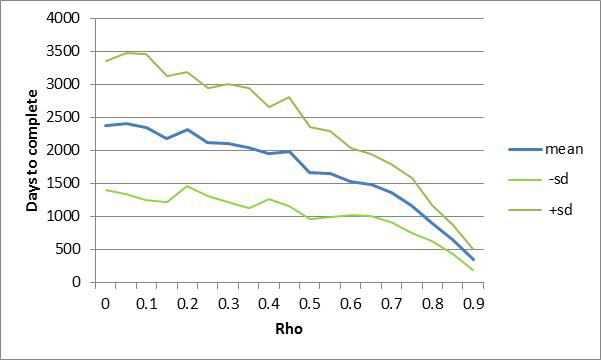
\includegraphics[width=0.7\textwidth]{ChapterConnectedModels/Figures/FirmGame13}}
\caption{Firms compete to reach centre of market. Number of days to success on vertical axis, value of $\rho$ on horizontal. Mean and S.D. for a hundred randomisations of each value point. Three different noise levels. Note for figure \ref{fig:fg13}, days to complete are an order of magnitude higher than for \ref{fig:fg12}. \label{fig:FirmGame1}}%
\end{figure}

In this example there are five key factors that impact on revenue. The first is a Firm's own actions - just moving to a new spot. The second comes indirectly from the actions of other Firms: they may move to a location that leads People to shift demand to them, and this in turn may make other Firms' revenue-flow negative where it would otherwise have been positive. The other three factors all relate to the connection between People's demand levels and noise. If People are using pure constrained utility - thus providing a crystal-clear demand signal - Firms have no problems making correct decisions about changes in revenue. However, if demand is less clear than this from turn to turn, revenue signals become less reliable. More than this, as noise increases, the value of $\rho$ - the level of \gls{lov} in the model - begins to determine Firms' success rate.

In the model framework, noise naturally appears when using the hill-climber algorithm, and it is noisier the less iterations are used. As section \ref{sec:optimisingbundles} explained, the algorithm starts by guessing budget slices for all available goods. With fewer iterations, these guesses are further from the `perfect' optimisation, and thus demand fluctuates. It is in running hill-climber algorithm models that the impact of noise on Firm optimisation becomes apparent. However, for the sake of computational expense and feasibility of large parameter sweeps, a noise term has been added to the constrained utility methods.\footnote{While a noise term can be added to the constrained algorithm, it is quite hard to make it economically sensible. This requires staying in budget: the hill-climber algorithm does this by design. Adding noise to constrained utility, however, may mean People appearing to spend slightly too much or too little. Avoiding this is actually a large optimisation problem in itself, since there is no way to `read back' from constrained good quantities.} 

The noise term just adds a random fluctuation to the optimal good quantities the constrained algorithm finds. For instance, if $noise=0.5$, the optimal quantity is randomised in a range of plus or minus half its total value.

Firm and Person numbers are the final two factors, both impacting on demand noise level, if any is present. Both have a similar effect, for different reasons. Increasing the number of People means a larger source of demand for each Firm's goods, thus tending to average any noise out as these rise. Rather less intuitively, increasing Firm numbers reduces noise when using the hill-climber algorithm simply because the variance of size of budget slices drops. A budget randomly split between two Firms will have a much higher variance than one split between ten or a hundred. Constrained utility noise is equally lower, as it is applied proportionally to the quantity of optimised good amount.

Figure \ref{fig:FirmGame1} graphs the average number of days it took both Firms to get inside the line of People, for a range of values of $\rho$ up to 1, in $R^1$. A hundred randomisations were averaged for each value of $\rho$. Three different noise levels were tested: it can be seen that when no noise is present, $\rho$ makes no difference to the success of Firms' decisions. As the noise level increases, however, $\rho$ begins to be important. High levels ($\rho \rightarrow 1$) present no problem, regardless of noise level. However, as \gls{lov} increases ($\rho \rightarrow 0$) noise increasingly interferes in a Firms' ability to correctly identify revenue-improving positions.

Why does $\rho$ have this effect? Because if \gls{lov} is higher, any change in a Firm's location has a higher external effect on the demand the other Firm faces. This makes the signalling less clear and, in the presence of noise, more likely to cause a Firm to interpret information from the market falsely.
%The implications of this are discussed in more detail in the final chapter, in the context of the various approaches to coordination taken in the thesis. 
%Now, is this because of $\rho$'s effect on People's choices, or its effect on how Firms' decisions interact with each other?
%In contrast to objective optima possible in analytic approaches, in this situation Firms cannot know whether their current revenue has reached a point of final optimum. In practice this means they will always need to `test the waters' looking for further improvements. A consequence of this is that they may cede revenue, and leave a space for others to exploit. No one Firm can act without changing the situation others face. Attempting to seek revenue improvements thus becomes a constant battle, unable ever to stabilise.
%There is, however, a region of stability within which this battle for revenue takes place, and once a Firm has found it, they able to hold that position.
%Note that Firms test only for an increase in sales since the last turn. Outgoing costs do not enter into the calculation: wages are fixed, and so it makes no sense for Firms to have to pay them.
\section{Summary \label{sec:partialconcs}}

%Hotelling bit:
A transparent location example is used as a way to think about other possible \gls{dmr} decisions involving price and wage setting. There are other reasons why varying good price and wages present problems, discussed further in section \ref{sec:partialtogeneral}, but the \gls{dmr} model suggests that noise issues exist in any market where Firms require some form of `sonar' signal back from their actions. While Firms in section \ref{sec:mobFirms} are able to optimise their location, the outcome is far from the cleanly deduced stable competition outcome examined in Hotelling's original two-firm line model. As section \ref{sec:firmsLoV} explored, in sticking to a \gls{dmr} approach, Firms have only a narrow view of the effect of their actions. 

One option is to allow each Firm to separately pursue its optimal outcome until some maximum is reached while holding all other actions static. This would allow them to fully optimise having removed any possible conflicting signals. As mentioned, single Firms certainly have no problem identifying their optimal position: it is only in the presence of other Firms that it becomes challenging. This method of fully separate decisions is used in Plummer \emph{et al}.  (\citeyear{plummer_rationality_2012}), taking their idea from Schendel and Balestra (\citeyear{schendel_rational_1969}). They suggest ``retailers temporarily alter their prices, observe the effect on their profit objective before competitors respond, and then use this information to institute a price change'' (p.543), thus avoiding conflicting signals.

However, the goal of the thesis is to examine how to let agents make decisions independently. The \gls{dmr} example is a simple case, but it presents even more difficulties for the transmission belt model in chapter \ref{chapter:connectedModels} where constant interacting signals are an unavoidable element of the model's construction. 

%Monocentric bits:
In the `mobile People' models, an agent approach makes it relatively easy to equip agents with a `second nature' reaction to proximity (section \ref{sec:1st2ndnature}). The density cost produces a beguiling outcome, able to produce spatial equilibrium with no market arbitrage. Urban economic models built on the spatial equilibrium assumption also rely on the `first nature' properties of land - though land cost itself is `second nature': it is a property of demand. The density cost approach goes some way to capturing this, in a scenario where land is otherwise homogenous (having no intrinsic value that might make one spot more valuable than another). 
%What does `arbitrage' look like, algorithmically? Is this a form of spatial arbitrage? No, it's not! 

The underlying message is that, if agents are provided with an ability to find utility opportunities better than their own, in a situation where their actions interact spatially, equilibrium can result without the need for any specific market mechanism. As section \ref{sec:rationalchoices}, the density cost produces this outcome through the interaction of People's optimising choices and the externalities of those choices. The outcome works precisely \emph{because} of its sequential nature: the choice set of the next Person is effected by the previous Person's decision. As with the way in which strategy considerations are avoided when using \gls{eos} in chapter \ref{chapter:connectedModels}, actually ruling out game-theoretical considerations is suited to spatial analysis and Oeffner's point about `irreducible uncertainty'. 

As section \ref{sec:litbits} explained, Fujita \emph{et al.} note that the `monocentric' assumption cannot help directly if one wants to understand endogenous forces leading to settlement location, number and size. But Blaug makes an important point: the power of the monocentric model is precisely in its clarity. Von Thunen knew the `isolate state' was abstract: 

\begin{quote}
``in reality, Thunen observes, differences in fertility of the soil which are not themselves related to location will give rise to ground rent in the same manner as do differences in proximity to the central town.'' (\citealt{blaug_economic_1997} p.598)
\end{quote}

From this point of view, the `monocentric' approach is not about a specific settlement pattern, but understanding the polarity and magnitude of spatial forces. The conclusion returns in detail to the models in this chapter, placing them in the context of the following chapter's findings as well as the aims and objectives of the thesis.
%Booya!
